\documentclass[a4paper]{article}

%% Language and font encodings
\usepackage[english]{babel}
\usepackage[utf8x]{inputenc}
\usepackage[T1]{fontenc}
\usepackage{float}
%% Sets page size and margins
\usepackage[a4paper,top=3cm,bottom=2cm,left=3cm,right=3cm,marginparwidth=1.75cm]{geometry}
\usepackage{tabularx}
%% Useful packages
\usepackage{enumitem}
\usepackage{amsmath}
\usepackage{amsthm}
\usepackage{fancyhdr}
\pagestyle{fancy}
\usepackage{eqnarray}
\usepackage{float}
\usepackage{esint}
\usepackage{wrapfig}
\usepackage{gensymb}
\usepackage{lipsum}
\usepackage{amssymb}
\usepackage{array}
\usepackage{tikz}
\usepackage{pgfplots}
\pgfplotsset{compat=1.7} % So the compiler stops throwing warnings
\usepackage[colorlinks=true, allcolors=blue]{hyperref}
\usepackage{graphicx}
\usepackage{amsmath}
\usepackage{amssymb}
\usepackage{graphicx}
\usepackage[colorlinks=true, allcolors=blue]{hyperref}
\usepackage{mathtools}
\DeclareMathOperator{\Proj}{Proj}
\DeclareMathOperator{\lcm}{lcm}
\DeclareMathOperator{\sgn}{sgn}
\DeclareMathOperator{\Span}{span}
\DeclareMathOperator{\sinc}{sinc}
\DeclareMathOperator{\nullity}{nullity}
\DeclarePairedDelimiter\floor{\lfloor}{\rfloor}
\DeclareMathOperator{\Res}{Res}
\DeclareMathOperator{\rank}{rank}
\DeclareMathOperator{\Ker}{Ker}
\DeclareMathOperator{\R}{R}
\DeclareMathOperator{\Tr}{Tr}
\DeclareMathOperator{\Id}{Id}
\DeclareMathOperator{\diag}{diag}
\DeclareMathOperator{\Log}{Log}
\DeclareMathOperator{\sech}{sech}
\DeclareMathOperator{\Var}{Var}
\newtheorem{ans}{Answer}[section]

\definecolor{darkblue}{RGB}{	0, 0, 139}
\newtheoremstyle{new}% <name>
{2pt}% <Space above>
{2pt}% <Space below>
{\color{darkblue}}% Body font
{}% <Indent amount>
{\bfseries\color{black}}% Theorem head font
{:}% <Punctuation after theorem head>
{.5em}% <Space after theorem headi>
{}% <Theorem head spec (can be left empty, meaning `normal')>
\theoremstyle{new}
\newtheorem{qns}{Problem}[section]
\setlength{\parindent}{0cm}
\title{\textbf{Problem Sheet for IB Physics A}}
\author{Tai Yingzhe, Tommy (ytt26)}
\date{}
\begin{document}
\maketitle
\tableofcontents
\newpage
\section{Experimental Methods}
\subsection{Ideal Operational Amplifier Circuits}
\begin{qns}[Ideal Operational Amplifier Circuits]\leavevmode
\begin{enumerate}[label=(\alph*)]
\item Show that 1. the voltage across $R_{load}$ is an excellent measurement of $V$ provided that $R_{load}>>R_{out}$; 2. maximum power is transferred into $R_{load}$ when $R_{load}=R_{out}$. In what physical situations might these results be important?
\item Determine the behaviour of this circuit for position 1 of the switch and again for position 2. How will the frequency and level of the input signal $V_{in}$ be expected to affect the output signal?
\item Show by conserving current and using the Golden Rules that a buffer has unit gain and infinite input impedance. 
\item What problems might you experience when using the circuits below (second one is an integrator) and how might you either take advantage of these or mitigate against them?
\end{enumerate}
\end{qns}
\begin{figure}[H]
    \centering
    \includegraphics[scale=0.45]{1_1.PNG}
\end{figure}
\begin{ans}\leavevmode
\begin{enumerate}[label=(\alph*)]
\item Using the potential divider rule, $V_{load}=(1+\frac{R_{out}}{R_{load}})^{-1}V\approx V$ for $R_{load}>>R_{out}$.\\[5pt]
The power is $$I^2R_{load}=\frac{R_{load}V^2}{(R_{load}+R_{out})^2}$$
and upon extremizing,
$$\frac{dP}{dR_{load}}=0\implies (1-\frac{2R_{load}}{R_{load}+R_{out}})=0\implies R_{out}=R_{load}$$
$$\frac{d^2P}{dR_{load}^2}=-\frac{4V^2}{(R_{load}+R_{out})^3}+\frac{6R_{load}V^2}{(R_{load}+R_{out})^4}<0$$ 
Power matching is used mainly in 3 situations:
\begin{itemize}
    \item where the signal levels are very small so any power loss results in a much worse signal-to-noise ratio;
    \item where the signal at high frequency is connected through lines of appreciable self-capacitance and self-inductance to a load. Then it is possible to get large standing waves due to reflections from the load which can make the source-to-load power transfer low;
    \item where signals are very large, say at the output stage of a transmitter, and where the maximum efficiency is desirable on economic grounds.
\end{itemize}
\item Draw two separate diagrams for position 1 and position 2. For former, by the Golden Rules, $V_-=0$ and the (-) terminal draws no current, i.e. $\frac{V_{in}-0}{R}=\frac{0-V_{out}}{R}$. Then, the gain $\frac{V_{out}}{V_{in}}=-1$, so the amplitude will be scaled by $-1$. The frequency is unchanged. For the latter, since by the Golden Rule $V_+=V_-=0$, there is no potential drop across $R$ and since no current flows across $R$. We thus expect the gain to be $\frac{V_{out}}{V_{in}}=1$.
\item Consider a simple buffer design such that $V_2$ (the output) is fed back into the (-) terminal, while the (+) terminal has $V_1$. We thus have $V_2=A(-V_2+V_1)\implies\frac{V_2}{V_1}=\frac{A}{A+1}\approx1$ for very high $A$, hence unity gain. It appears that no current is drawn, and so has infinite input impedance. Buffer is helpful to isolate the signal generator from the load resistance.
\item \textbf{Left Hand Side}: The output is fed back into the ($+$) terminal, leading to positive feedback. But due to the design of the operational amplifier, the output voltage will saturate. Due to clipping, the resultant waveform is square waves (useful if desired). We can't use Golden rule since positive feedback is unstable. \\[5pt]
\textbf{Right Hand Side}: Assuming the operational amplifier is ideal, the ($-$) terminal draws no current, and so let the current flow along $R$ and $C$ to be $I_1$ and $I_2$ respectively. We have
$$\frac{V_{in}-V_X}{R}=I_1=I_2$$
but $V_{out}-V_X=-\frac{1}{C}\int_0^tI_1dt=-\frac{1}{C}\int_0^t\frac{V_{in}-V_X}{R}dt$. When $A$ is very large, $V_X\rightarrow 0$ and so
$$V_{out}=-\frac{1}{RC}\int_0^tV_{in}dt$$
which behaves like an integrator. For AC voltages of the exponential form $\sim e^{i\omega t}$, we have $V_{out}=-\frac{1}{i\omega RC}|V_{in}|e^{i\omega t}$. This is undefined for $\omega=0$ and leads to saturation. Low frequency voltages may also saturate. To avoid this issue, we add a resistor parallel to the capacitor, at the expense of not exact integration. The use of the integrator is to perform calculus operations in analogue computers, as well as, to integrate signals. 
\end{enumerate}
\end{ans}
\begin{qns}[Negative Impedance Convertor]
Show that the input impedance for this circuit is $-Z$. If $Z$ represents a capacitor, show that this circuit simulates an inductor to the extent that the current $I_{in}$ lags behind the applied voltage $V_{in}$.
\end{qns}
\begin{figure}[H]
    \centering
    \includegraphics[scale=0.5]{1_2.PNG}
\end{figure}
\begin{ans}
Assuming negative feedback dominates, or else question can't be solved. Since it is an ideal operational amplifier, neither terminal draws current ideally since $V_-\approx V_+$. We have $I_{in}=\frac{V_+-V_{out}}{R}$. We clearly have $V_+=V_{in}$ since (+) terminal draws no current. Let $I_2$ be the current that flows up through $R$, then down through $Z$, we have 
$$I_2=\frac{V_{out}-V_-}{R}=\frac{V_--0}{Z}$$
where we assume (-) terminal draws no current. But, $V_-=V_+=V_{in}$. We thus have $\frac{V_{out}-V_{in}}{R}=\frac{V_{in}}{Z}$. We have $I_{in}=\frac{V_{in}-V_{out}}{R}=-\frac{V_{in}}{Z}$. Evaluating $Z_{in}$,
$$Z_{in}=\frac{V_{in}}{I_{in}}=-Z$$
(shown). If $Z=\frac{1}{i\omega C}$, then $Z_{in}=\frac{i}{\omega C}$. We thus have the current to lag behind the applied voltage by $\pi/2$ phase, as desired. In the perspective of phase, we have the circuit behave like an inductor.
\end{ans}
\newpage
\subsection{Non-Ideal Operational Amplifier Circuits and Feedback}
\begin{qns}[Non-ideal Inverting]
Consider this circuit that uses a non-ideal op-amp of open-loop gain $A$ and input resistance $r_{in}$ and a negative feedback resistor $R_2$ in the usual inverting configuration. Show that the input impedance of this system can be written as
$$Z_{in}=R_1\bigg(1+\frac{r_{in}R_2}{R_1(r_{in}(1+A)+R_2)}\bigg)$$
As the op-amp becomes more ideal, does this tend to the value you would expect.
\end{qns}
\begin{figure}[H]
    \centering
    \includegraphics[scale=0.5]{1_3.PNG}
\end{figure}
\begin{ans}
Let node X be the node closest to the (-) terminal, then conserving current gives
$$\frac{V_{in}-V_X}{R_1}+\frac{V_{out}-V_X}{R_2}=\frac{V_X-V_+}{r_{in}}$$
but $V_+=0$ and $V_{out}=A(V_+-V_X)=-AV_X$. Hence,
$$r_{in}R_2(V_{in}-V_X)-R_1r_{in}V_X(A+1)=R_1R_2V_X\implies r_{in}R_2V_{in}=V_X[r_{in}[R_2+R_1(A+1)]+R_1R_2]$$
By definition of input impedance, we have $$Z_{in}=\frac{V_{in}}{I_{in}}=\frac{V_{in}R_1}{V_{in}-V_X}=\frac{R_1}{1-(V_X/V_{in})}$$
Then
$$\frac{V_X}{V_{in}}=\frac{r_{in}R_2}{r_{in}[R_2+R_1(A+1)]+R_1R_2}\implies\bigg(1-\frac{V_X}{V_{in}}\bigg)^{-1}=1+\frac{r_{in}R_2}{R_1[R_2+r_{in}(A+1)]}$$
For an ideal operational amplifier, i.e. $A\rightarrow\infty$ and $r_{in}\rightarrow\infty$ (with the former condition being more important for the approximation), we then have $Z_{in}\approx R_1$ as expected.
\end{ans}
\newpage
\begin{qns}[Feedback]\leavevmode
\begin{enumerate}[label=(\alph*)]
\item Consider the system below, where $A$ is the open-loop gain, is nominally $10^4$ but can vary by $\pm 20$ \%, and $\beta$ is exactly -0.1. What is the nominal closed-loop gain of the system and the range of its variation?
\item Two methods of applying negative feedback to obtain the same overall gain in a multistage system are shown below. By considering the phase of the output of each amplifier stage relative to its input and the impact of uncertainty in the characteristics of the components used, suggest qualitative arguments for and against the use of each circuit. Under what circumstances might each of the different arrangements be preferred and why?
\end{enumerate}
[Hint: For each circuit how are small variations in the phase and open loop gain at each stage combined together? What does this mean for the overall uncertainty in the gain and phase of the entire circuit?]
\end{qns}
\begin{figure}[H]
    \centering
    \includegraphics[scale=0.5]{1_4.PNG}
\end{figure}
\begin{ans}\leavevmode
\begin{enumerate}[label=(\alph*)]
\item We have the output to be equal to $A$ times the input plus $\beta$ times output. The nominal closed loop gain is the ratio of output to input, which is $G=\frac{A}{1-A\beta}$. For this example, this is $\frac{10^4}{(1+10^3)}=9.990$. We then have
$$\frac{\Delta G}{\Delta A}=\frac{1}{1-A\beta}+\frac{A\beta}{(1-A\beta)^2}=\frac{1}{(1-A\beta)^2}$$
for $\frac{\Delta A}{A}=0.2$, we have $\Delta G=\frac{0.2\times10^4}{(1+10^3)^2}=2.0\times10^{-3}$ and hence $G=9.990\pm0.002$. We essentially traded the uncertainty of $G$ with the magnitude of $A$. This is to stabilize the amplifier.
\item Each amplifier has an inherent time delay between input and output, hence a phase difference. Feedback intends to correct this error. For the circuit on the left, each amplifier has its own feedback, as compared to the circuit on the right. This small time delay in each amplifier may build up after $n$-stages, such that the overall phase shift to become $\pi$, and hence inducing positive feedback.\\[5pt]
If we were to compare the effective gains, we will have $\frac{A^n}{(1-A\beta_1)^n}$ versus $\frac{A^n}{1-A^n\beta_2}$ and so $\frac{dG_1}{G_1}=\frac{n}{1-A\beta_1}\frac{dA}{A}$ and $\frac{dG_2}{G_2}=\frac{n}{1-A^n\beta_2}\frac{dA}{A}$. To achieve the same overall gain, we have $(1-A\beta_1)^n=1-A^n\beta_2$ and hence $\frac{dG_2/G_2}{dG_1/G_1}=\frac{1}{(1-A\beta_1)^{n-1}}$. For $n>1$ and $|A\beta_1|>>1$, then for the same change in $A$ and since $G_1=G_2$, we have $dG_2<dG_1$, i.e. the gain on the right is smaller for a change in $A$, i.e. more stable and precise.
\end{enumerate}
\end{ans}
\newpage
\begin{qns}[Relaxation Oscillator]
The circuit shown is a “relaxation” oscillator. When the voltage supply to the op-amp (note, this is not shown) is turned on, the op-amp output will saturate at either its $+15V$ or $-15V$ limit. If the output saturates at $+15V$, for example, the capacitor will then start charging up towards $+ 15V$. 
\begin{figure}[H]
    \centering
    \includegraphics[scale=0.9]{1_5.PNG}
\end{figure}
By sketching the waveforms at the inverting “−” pin and at the op-amp output as a function of time (from the time that the capacitor begins to start charging), describe what happens in the circuit at later times.\\[5pt]
Show, by considering your sketches, that the circuit will oscillate with a period equal to $2.2 RC$. What shape will this periodic waveform have?\\[5pt]
[Hint: Do not attempt to used the Golden Rules – the op-amp output is saturated, and so the Golden Rules will no longer be appropriate here.]
\end{qns}

\begin{ans}
The operational amplifier is designed to give maximum voltages $V_{out}=\pm15V$. Since the two resistors of 10k are equal in value, then by the potential divider rule, we have $V_+=\frac{1}{2}V_{out}=\pm7.5V$. We simply have
$$V_0=R\frac{dQ}{dt}+\frac{Q}{C}\implies\frac{Q}{C}=V_0(1-e^{-t/RC})$$
Initially, the capacitor charges up, and follows the equation above. When the capacitor charges beyond $V_C=+7.5V$, $V_->V_+=+7.5V$ and so $V_{out}=A(V_+-V_-)<0$. Since $A$ is ideally infinite, we have a negative infinity output voltage, which have to saturate to $-15V$. Assuming it does so instantly, then $V_+$ is now $-7.5V$. This results in the capacitor to be discharged. Similarly, when $V_C$ goes beyond $-7.5V$, $V_-<-7.5V=V_+$ and so $V_{out}$ reaches to positive infinity and saturates towards $+7.5V$.\\[5pt]
We choose $t_1$ and $t_1+\tau$ (where $\tau$ is half the period of the $V_C$ waveform, i.e. the time it takes to reach from $+7.5V$ to $-7.5V$, or vice-versa) such that
$$-\frac{V_0}{2}=V_0(1-e^{-t_1/RC})$$
$$\frac{V_0}{2}=V_0(1-e^{-(t_1+\tau)/RC})$$
We thus have $1.5=e^{-t_1/RC}\implies 2\tau=2.2RC$.
\end{ans}
\subsection{Random Errors}
\begin{qns}\leavevmode
\begin{enumerate}[label=(\alph*)]
\item You are designing an experimental procedure to measure the temperature of an item. Is it better to have a set of ten measurements of its temperature each with a random error of $10mK$, or two each with an error of $4 mK$, or one with an error of $2 mK$? Explain your reasoning clearly.
\item Ten experimenters make a measurement of quantity $Q$ using method A. The values of $Q$ they find are:
$$3.91,~4.29,~3.75,~4.28,~3.68,~4.10,~3.61,~4.19,~4.18,~4.01$$
Each experimenter then moves on to measure $Q$ using method B, finding the following values:
$$4.05,~4.11,~4.05,~4.10,~4.04,~4.06,~4.03,~4.09,~4.07,~4.06$$
For each method, estimate the mean value of $Q$ found and the error on this mean. Is there any quantitative evidence for a systematic difference between the methods A and B? Is there any evidence for a systematic difference between the experimenters? [Hint: You should think about how you might assess whether a systematic error exists.]
\end{enumerate}
\end{qns}
\begin{ans}\leavevmode
\begin{enumerate}[label=(\alph*)]
\item Computing the errors, we have $\frac{10}{\sqrt{10}}\approx 3$ mK, $\frac{4}{\sqrt{2}}\approx 3$ mK and $2mK$ respectively. Although the third one seems to have the smallest error, the first one is clearly better since it has much more measurement points.
\item We have
$$\overline{Q}=\frac{1}{N}\sum_{i=1}^Nx_i$$
$$\sigma^2=\frac{1}{N-1}\sum_{i=1}^N(x_i-\overline{Q})^2\implies\Delta Q=\frac{\sigma}{\sqrt{N}}$$
For Method A, we have
$\overline{Q}=4$, $\sigma=0.250821$, and so $\Delta Q=\frac{\sigma}{\sqrt{10}}=0.08$. Thus, $\overline{Q}=4.00\pm0.08$. For Method B, we have $4.066\pm0.008$. The difference in mean is 0.066, and by adding variances, i.e. $\sqrt{0.026331^2+0.250821^2}\approx0.08$. The difference between the means lie in one standard deviation 0.08, so no evidence for systematic error between the two methods. As for systematic difference between the experimenters, it is hard to determine unless the list measurement are paired correctly. If they are, we can use covariance.
\end{enumerate}
\end{ans}
\newpage
\begin{qns}\leavevmode
\begin{enumerate}[label=(\alph*)]
\item Calculate the value of f and estimate its error for the given values of $x\pm\sigma_x$, $y\pm\sigma_y$, etc. In each case sketch and annotate a histogram of what you think the distribution of the values of $f$ might be expected to look like explaining its key features.
$$f=x-y,\text{ for }x=2.0\pm0.2,~y=5.0\pm0.3$$
$$f=2x/y,\text{ for }x=4.0\pm0.2,~y=2.0\pm0.1$$
$$f=x^3\text{ for }x=10\pm1$$
$$f=zx\ln(y)\text{ for }x=1.5\pm0.1,~y=10\pm1,~z=2.0\pm0.1$$
\item If $\theta = 1.56\pm0.01$ radians, what are the errors on $\sin\theta$, $\cos\theta$ and $\theta$? As for part (a), sketch and annotate histograms depicting what you think the distribution of the values of $\sin\theta$, $\cos\theta$ and $\theta$ might look like.
\item If $f = [\sin (x + y)] /\sin x$, $x = 30.0\degree \pm 0.5\degree$ and $y = 20\degree \pm 2\degree$, estimate the error in $f$ by explicitly determining the changes in $f(x,y)$ for changes in its arguments of $\sigma_x$, and $\sigma_y$ respectively.
\end{enumerate}
\end{qns}
\begin{ans}\leavevmode
\begin{enumerate}[label=(\alph*)]
\item $f=2.0-5.0=-3.0$ with $(\Delta f)^2=(\Delta x)^2+(\Delta y)^2\implies\Delta f=0.4$, hence $f=-3.0\pm0.4$. Symmetric Gaussian\\[5pt]
$f=\frac{2x}{y}=\frac{2(4.0)}{2.0}=4$ with $(\Delta f/f)^2=(\Delta x/x)^2+(\Delta y/y)^2\implies\Delta f=0.3$, hence $f=4.0\pm0.3$. Assuming $x$ and $y$ have independent Gaussian distributions, then resultant is a symmetric Gaussian.\\[5pt]
$f=x^3=1000$ with $\Delta f=3x^2\Delta x=300$, hence $f=1000\pm300$. Since we assumed that $x$ follow a Gaussian distribution, $f$ would have an asymmetric distribution due to the scaling of $x^3$.\\[5pt]
$f=zx\ln(y)=6.908$ with $(\Delta f)^2=(z\ln y \Delta x)^2+(zxy^{-1}\Delta y)^2+(x\ln y\Delta z)^2\implies\Delta f\approx 0.6$, hence $f=6.9\pm0.6$. Assuming independent Gaussian distributions for $x$, $y$ and $z$, the asymmetry is due to the $\ln(y)$ term in the product.
\item The distribution of $\sin\theta$ will be skewed towards 1 (hard limit). $\cos\theta=0.010786$ with $\Delta\cos\theta=\sin\theta\Delta\theta=0.01$ and so $\cos\theta=0.01\pm0.01$. This is valid since $\cos\theta$ is approximately linear in this range of $\theta$, i.e. nearly symmetric distribution. $\tan\theta=92.620496$, assuming symmetric errors, then $\tan\theta$ is skewed towards $\tan(1.55)$ since rate of increase is smaller for smaller $\theta$.
\begin{figure}[H]
    \centering
    \includegraphics[width=\linewidth]{1_7.PNG}
    \caption{Histograms illustrating the distribution for $\sin\theta$ (Left), $\cos\theta$ (Middle), $\tan\theta$ (Right).}
\end{figure}
\item Let $f=f(x,y)$. $f(30\degree,20\degree)=1.532089$, $f(30.5\degree,20\degree)=1.5203276$, $f(30\degree,22\degree)=1.5760215$ and
$$(\Delta f)^2=[f(30.5\degree,20\degree)-f(30\degree,20\degree)]^2+[f(30\degree,22\degree)-f(30\degree,20\degree)]^2\implies\Delta f=0.045$$
Hence, $f=1.53\pm0.05$.
\end{enumerate}
\end{ans}
\newpage
\subsection{Systematic Errors and Digital Sampling}
\begin{qns}
You are designing an optical sensor for night-time surveillance in the infra-red at a wavelength of $20\mu m$. You want the collecting optics to be as large as possible to receive as many photons as possible from your targets and so reduce the uncertainty in the signal from them. But there are many other potential sources of error that may constrain your data, for example:
\begin{itemize}
    \item the local environment may not be dark, either because of scattered light from natural and artificial sources, or simply because it has a finite temperature; 
    \item the structural components and optics of your sensor will be radiating in the infrared, and as the environment and your sensor cools down during the night this radiation can change at rates from DC to several Hz;
    \item electronic interference may be present from AC mains, computers etc;
    \item the local environment will likely not be stable, e.g., with lights being switched on intermittently, passing cars, and changing weather.
\end{itemize}
Discuss, using quantitative arguments where appropriate, which of these may be significant issues, and, for these, suggest some ways by which these the impact of these systematic errors might be reduced.
\end{qns}
\begin{ans}
\textbf{Local environment may not be `dark' due to presence of background noise:} Measure the average background noise over various regular intervals, and take a mean. This background value is deducted from subsequent measurements. Note that this white noise (thermal noise is white noise) might be larger than the actual signal.\\[5pt]
\textbf{Structural components and optics of sensor radiate at infrared:} This cannot be reduced, unless the equipment is kept as cool as possible, in a temperature range the internal components allow. Shield the equipment thermally, by preventing heat transfer via conduction, convection and radiation. This can be done using a thin foil as a shield and an insulated support.\\[5pt]
\textbf{The infrared radiation can change at rates from DC to several Hz:} Sample at the rate and frequency of this thermal noise. For data with different timescales, use Fourier transform to filter. We could use filter to remove the noise directly.\\[5pt]
\textbf{Electronic interference may be present from AC mains, etc: } Shield camera appropriately away from external electric fields by using a Faraday cage. Stray magnetic fields may be removed using twisted pair wires. Coaxial cables may also be used for better shielding.\\[5pt]
\textbf{Local environment may not be stable:} Ensure detector detects signal at a very narrow wavelength range to minimize interference with other wavelengths. For a  particular wavelength, take average over entire region or a large time range. Use this average to compare with the localized time and region.
\end{ans}
\newpage
\begin{qns}\leavevmode
\begin{enumerate}[label=(\alph*)]
\item A signal has the following frequency spectrum (note, the identical negative frequency components are not shown in the schematic spectrum below). The signal is sampled at 200 MHz (i.e. $<$ than twice the maximum frequency in the spectrum). Remembering that the frequency spectrum for a real signal will contain both negative and positive values, draw an annotated sketch of the Fourier spectrum of the sampled signal, identifying the original signal’s convolution images, and use this to determine whether or not this sampling frequency will be adequate for eventual recovery of the signal from its sampled version?\\[5pt]
Explain whether sampling frequencies of (i) 100 MHz or (ii) 150 MHz would be useful frequencies with which to sample the signal without losing any information.
\begin{figure}[H]
    \centering
    \includegraphics[scale=0.5]{1_9.PNG}
\end{figure}
\item  A radio telescope observes the intensity of a source over a frequency band from $A$ Hz to $A+10^9$ Hz. The signal is sampled directly with four levels. Outline clearly in words the argument that suggests that the sampler must have a minimum bit rate of at least $4(A+10^9)$ bits s$^{–1}$.
\item An ADC is being used to sample a constant voltage output, $V_T$ = 2.75 V from a thermistor at some temperature T. It has 11 equally spaced quantization levels between minus 0.50 V and $+$10.49 V (i.e. it gives an output of 0 V for all inputs between $-$0.5 V and 0.5 V, an output of 1V for all inputs between 0.5-1.5 V, an output of 2 V for all inputs between 1.5-2.5 V etc).\\[5pt]
By considering what happens to the average value of the output of the ADC if a noise voltage uniformly distributed between $\pm$0.5 V is added to $V_T$ before digitization, show that it can be beneficial to add a small amount of noise to a signal prior to sampling it. Explain in qualitative terms under what circumstances this might be a helpful strategy and how one might go about selecting what type of noise to add.
\end{enumerate}
\end{qns}
\begin{ans}\leavevmode
\begin{enumerate}[label=(\alph*)]
\item Here, we vary sampling frequency. The sampled signal is the true signal multiplied by the sampling comb function. By convolution theorem, the Fourier transform of the sampled signal is the frequency spectrum (symmetric) given convolved with another comb function. We generalize the problem as follow: the original signal consists of two asymmetric humps placed symmetrically about $\omega=0$, and are bounded by the two edges $\omega_{min}$ and $\omega_{max}$.\\[5pt]
It is very likely for the $n$th convolution image of the left hump to overlap with the right hump of the original signal. We consider separately two cases:\\[5pt]
Case 1: $n\omega_s>\omega_{max}$, then the leftmost edge of the left hump of the $n$th convolution image (at frequency $n\omega_s-\omega_{max}$) coincides with the rightmost edge of the right hump of the original signal (at frequency $\omega_{max}$), i.e. check $n\omega_s-\omega_{max}\geq\omega_{max}$.\\[5pt]
Case 2: $n\omega_s<\omega_{max}$, then the rightmost edge of the left hump of the $n$th convolution image (at frequency $n\omega_s-\omega_{min}$) coincides with the leftmost edge of the right hump of the original signal (at frequency $\omega_{min}$), i.e. check $n\omega_s-\omega_{min}\leq\omega_{min}$.\\[5pt]
For $\omega_s=200$ MHz, we have case 1 to be true for $n\geq 2$, i.e. $200n\geq304$. For $n=1$ (case 2), we have $200\leq 296$, which is also satisfied. For $\omega_s=150$ MHz and 100 MHz, we can find an $n$ that satisfy $n\omega_s\leq 296$. The smallest $n$ is 3 and 2 for $\omega_s=100$ MHz and 150 MHz respectively. Hence, no overlapping of convolution images will be observed for 200 MHz but there will be for 100 MHz and 150 MHz.
\newpage
\item Nyquist's Theorem say we need to sample signal at a rate that is at least twice as fast as the maximum frequency component present. To distinguish between the four signals, we need two bits and hence the minimum bit rate necessary is two times $2(A+10^9)$ bits per second. 
\item Given that: for $V\in[0.5,1.5]$, $V_{out}=1$ V; for $V\in[1.5,2.5]$, $V_{out}=2$ V; for $V\in[2.5,3.5]$, the $V_{out}=3$ V. Now a uniform symmetric noise is added in the voltage range $[2.75-0.5,2.75+0.5]$. But $2.5-(2.75-0.5)=0.25$ and $2.5-(2.75+0.5)=0.75$, and since it is symmetrically distributed, there is a 75 \% chance and 25 \% chance that the measured reading are in the intervals $[2.5,3.25]$ and $[2.25,2.5]$ respectively. Due to the quantization and `rounding', 3 V would be recorded 75 \% of the time and the 2V would be recorded 25 \% of the time, hence the average value would be $0.75\times 3+0.25\times 2=2.75$ V.\\[5pt]
This strategy of adding symmetric uniform noise, is helpful when a higher level of precision is desired compared to what the quantization levels can offer. 
\end{enumerate}
\end{ans}
\subsection{Eliminating Noise, Phase-Sensitive Detection}
\begin{qns}
Light from a distant source is focused onto a detector which counts the number of photons arriving in time intervals $\Delta t$. The light source has a sinusoidal variation of period $4\Delta t$ superimposed on a steady mean intensity, i.e. it consists of a noisy harmonic signal superimposed on a constant background. Given the photon counts in 100 successive time intervals below, estimate roughly the mean intensity of the source and the peak-to-peak range of its sinusoidal variation. (In the table below, the data should be read from left to right and then top to bottom, i.e. the final datum, 6, in the top row is followed by the datum 4 at the left of the second row, etc).
\begin{figure}[H]
    \centering
    \includegraphics[scale=0.6]{1_10.PNG}
\end{figure}
[Hint: Note that the phase of the sinusoidal signal does not change with time, and that its period is exactly equal to $4\Delta t$. Does this suggest a strategy for averaging the signals prior to analyzing them further?]
\end{qns}
\begin{ans}
Since the period is exactly equal to $4\Delta t$, we group the signals into blocks of four. Take the mean value of each block, and fit into the sine wave theoretical model i.e. $$A\sin\bigg(\frac{2\pi}{4\Delta t}t+\phi\bigg)+K$$
with $A$ being half of the desired peak-to-peak range and $K$ being the constant background. This fitting can be done using $\chi^2$ test (later). Otherwise, a quick estimate can be done by inspection.\\[5pt]
Such averaging throws out all frequencies not of period 4$\Delta t$. This is true since sinusoidal waves of different frequencies are orthogonal to each other. With more data, there is a smaller bandwidth of actual frequency.
\end{ans}
\begin{qns}
Write short notes on the following:
\begin{itemize}
    \item The basis for vibration isolation in sensitive mechanical experiments;
    \item Common strategies for removing systematic errors when designing experiments;
    \item The basis and rationale for phase-sensitive detection. 
\end{itemize}
In each case your text should be clear enough that a colleague who had not attended the Experimental Methods lectures would be able to identify the most critical aspects of the bases/strategies and understand in both qualitative and quantitative terms how and why they might be successful.
\end{qns}
\newpage
\begin{ans}\leavevmode
\subsubsection*{Vibration insulation:} 
In experiments where sensitive measurements need to be taken such as in interferometry, vibration insulation is required to reduce the mechanical noise, hence affecting the measurements. To reduce the amplitude of the vibration, we require a medium with very low resonant frequency as compared to the frequency of the undesirable external vibration. Further, higher damping in this medium would reduce undesirable resonant oscillations. This is achieved using air cushions where the oscillations comprise alternating adiabatic compressions and expansions, i.e. $PV^\gamma$ is a constant. In one cycle of vibration,
$$F=mg=PA\implies\frac{dF}{F}=\frac{dP}{P}=-\gamma\frac{dV}{V}\approx-\gamma\frac{dz}{dz_{eq}}$$
Applying Newton's second Law, we have $\ddot{z}=-\frac{\gamma g}{z_{eq}}z$ which gives $\omega_0=\sqrt{\gamma g/z_{eq}}$. For $z_{eq}=0.2$ m, we have $\omega_0=8.3$ rad/s since $\gamma_{air}=1.4$. This gives a $f=1.3$ Hz, which is sufficiently low.
\subsubsection*{Removing Systematic Errors:} 
\begin{itemize}
    \item Study the equipment and measurement instruments beforehand to identify zero errors and correct for them, and in general calibrate the instruments.
    \item Check the experimental set-up by measuring different quantities to make sure they are consistent with the desired experimental setup.
    \item Null methods can be used, where the indicating device need not be linear or well-calibrated and we attempt to make a measurement based on the indicating device coming to a null state.
    \item We can make the same measurement at different times to observe if there are any changes in the measured quantity due to environmental changes (ambient temperature) or changes in equipment (overheating) over time.
    \item We can make differential measurements so that the systematic error is cancelled out in the calculations.
\end{itemize}
\textbf{Phase Sensitive Detection:} Phase sensitive detection is a technique to reduce the effect of noise, that is being added after modulation. This works because noise isn't modulated (the idea of orthogonal function decomposition), giving us the desired frequency. Even noise very close to the desired frequency will be removed. If the noise is incoherent, it may be removed even if it coincides with the desired frequency.\\[5pt]
The circuit consists of Modulator One, an operational amplifier of gain $G$, Modulator Two, followed by a RC filter. Noise is added just before the operational amplifier. A reference oscillator (of frequency $\omega_r)$ connects the two modulators. This ensures both modulator waveforms have identical frequencies and a fixed phase relationship. $\omega_r$ is kept high to minimize $1/f$ noise.\\[5pt]
Modulator One is a sine wave such that after passing through the operational amplifier, it has a signal $V=GV_s\sin(\omega_rt+\phi)$. Modulator Two is a square wave (can be sinusoidal as long as same frequency and fixed phase relationship) such that the phase difference between that and the sine wave is $\phi$. After being modulated by the square wave, $V_{out}$ would represent the time-averaged value of the output after Modulator Two, which is given by 
$$\langle V_{out}\rangle=\frac{V_sG}{T}\bigg(\int_0^{\pi/\omega_r}\sin(\omega_rt+\phi)dt-\int_{\pi/\omega_r}^{2\pi/\omega_r}\sin(\omega_rt+\phi)dt\bigg)=\frac{2}{\pi}V_sG\cos\phi$$
One then change $\phi\mapsto\phi+\frac{\pi}{2}$ such that $\frac{\langle V_{out}\rangle}{2V_sG/\pi}=\cos\phi\rightarrow-\sin\phi$. This allow us to solve for $V_s$ and $\phi$. As for noise removal, suppose there exists noise at $\omega_r+\delta\omega$, then
$$\langle V_{n,out}\rangle=\frac{2G}{\pi}V_n\langle\cos(\delta\omega t+\phi)\rangle=\frac{2GV_n}{\pi\tau}\frac{1}{\delta\omega}\sin(\delta\omega\tau+\phi)$$
which approaches zero when $\tau\delta\omega>>1$, where $\tau=RC$ (the characteristic timescale of the low-pass filter). $\tau$ can be as small as 1 second to create an extremely narrow-band lock-in filter. The reference oscillator, nevertheless, must be phase stable for this length of time.
\end{ans}
\newpage
\subsection{Binomial, Poisson and Gaussian Processes}
\begin{qns}[Distribution]\leavevmode
\begin{enumerate}[label=(\alph*)]
\item After prolonged observation, it is found that events occur in a system at a mean rate of 13 per hour. Explaining your reasoning carefully, what is the chance of:
\begin{enumerate}[label=(\roman*)]
    \item 10 events happening in a given period of an hour;
    \item 3 events happening in a given period of 30 minutes;
    \item less than 4 events happening in a given period of 30 minutes.
\end{enumerate}
\item Cars pass at random times at an average rate of one per minute. The chance of a car stopping to give you a lift is one \%. Again, explaining your reason carefully, what is the chance that
\begin{enumerate}[label=(\roman*)]
    \item You will have got a lift after 60 cars have passed? What is the chance that you will still be waiting?
    \item You will have got a lift within one hour?
\end{enumerate}
\item For a Gaussian probability distribution:
\begin{enumerate}[label=(\roman*)]
    \item What is the chance of a value lying within $1.4\sigma$ of the mean?
    \item What is the chance of a value being greater than the mean plus $1.4\sigma$?
\end{enumerate}
\end{enumerate}
\end{qns}
\begin{ans}\leavevmode
\begin{enumerate}[label=(\alph*)]
\item Let $X$ be the discrete random variable that represents the number of occurrence of a event during a given time interval, i.e. $X\sim\text{Po}(\lambda)$. We have assumed
\begin{itemize}
    \item the number of occurrences in one time interval is independent of that occurring in any other disjoint time interval;
    \item the probability that the event occur during a very short time interval is proportional to the length of the time interval;
    \item the probability that more than one such events occur in such a short time interval is negligible.
\end{itemize}
We have $\lambda=13$ per hour:
\begin{enumerate}[label=(\roman*)]
\item $P(x=10)=\frac{13^{10}}{10!}e^{-13}=0.0859$\\[5pt]
\item Change $\lambda=6.5$ per 30 minute period. Then, $P(x=3)=\frac{6.5^3}{3!}e^{-6.5}=0.0688$.\\[5pt]
(iii) $P(X<4)=P(0)+P(1)+P(2)+P(3)=\frac{6.5^0}{0!}e^{-6.5}+\frac{6.5^1}{1!}e^{-6.5}+\frac{6.5^2}{2!}e^{-6.5}+\frac{6.5^3}{3!}e^{-6.5}=0.112$.
\end{enumerate}
\item
\begin{enumerate}[label=(\roman*)]
\item We draw a probability tree diagram, and we have a geometric series for the probability of getting a lift after 60 cars have passed.
$$P=\frac{1}{100}+\frac{1}{100}\bigg(\frac{99}{100}+\frac{99^2}{100^2}+...\bigg)=\frac{1}{100}\frac{-0.99^{60}+1}{-0.99+1}=0.453$$
The probability of still waiting after that is $1-0.453=0.547$.
\item Now let $Y$ be the discrete random variable that represents the number of cars per hour that give a lift. This is Poissonian with $\lambda=\frac{60}{100}$ per hour (60 cars have passed multiplied by the percentage that indeed gave a lift, i.e. 0.01). Here, we assume the same assumptions as in part (a). The probability of getting a lift in a hour is
$$1-\frac{0.6^0}{0!}e^{-0.6}=0.451$$
\end{enumerate}
\item 
\begin{enumerate}[label=(\roman*)]
\item Using the table of values, we quote $P(X\leq 1.4\sigma)=0.9192$, then
$$P(|X|\leq 1.4\sigma)=2(0.9192-0.5)=0.838$$
\item 
$$P(X\geq1.4\sigma)=1-P(X\leq 1.4\sigma)=0.0808$$
\end{enumerate}
\end{enumerate}
\end{ans}
\begin{qns}[Shot Noise]
In a scanning electron microscope, the average beam current is $I$, and $N$ pixels (= picture elements) of a sample are scanned per second. By considering the mean number of electrons contributing to each pixel, show that the signal-to-noise ratio per pixel cannot be better than $\sqrt{I/Ne}$, where $e$ is the charge of an electron.\\[5pt]
Suppose now you obtain a signal-to-noise ratio $R$ for a single pixel after measuring it for $t$ seconds. If you wish to scan $N$ pixels and measure, again with a signal-to-noise ratio $R$,
variations in $I$ from pixel to pixel that are typically 10 \% of the mean pixel intensity, how long will this take?\\[5pt]
[Hint: note that in the second part of the question the quantity you are interested in is ten times smaller than the mean signal level. Ans: 100$Nt$ seconds.]
\end{qns}
\begin{ans}
In one second, there are $\frac{I}{e}$ number of electrons in a current $I$. $N$ pixels are scanned and so the mean number of electrons per pixel in one second is $\frac{I}{Ne}$. Since this is like a rate process, the assumptions for a Poisson distribution are valid, and so $\lambda=\frac{I}{Ne}$ is the mean number of electrons per pixel per second. The standard deviation of a Poisson distribution is the noise, where $\sigma=\sqrt{\frac{I}{Ne}}$. The signal-to-noise ratio will be $\frac{I/Ne}{\sqrt{I/Ne}}=\sqrt{\frac{I}{Ne}}$.\\[5pt]
For the same signal-to-noise ratio $R$, we have
$$\sqrt{\frac{It'}{e}}(1/10)^{-1}=\sqrt{\frac{It}{e}}\implies t'=100t$$
We thus need to measure for a duration 10 times longer per pixel. Hence, a total of $100 Nt$ seconds.
\end{ans}
\begin{qns}[Gaussian and Johnson Noise]
Write short notes on the following:
\begin{itemize}
    \item The Gaussian distribution and the prevalence of its use in analyzing/interpreting experimental data;
    \item The roles of Johnson noise and shot-noise in limiting high precision experiments.
\end{itemize}
In each case make sure you give two examples of physical phenomena which demonstrate your discussion.
\end{qns}
\begin{ans}
\textbf{Gaussian Distribution:} The Gaussian distribution has a probability distribution
$$P(x;\mu,\sigma)=\frac{1}{\sqrt{2\pi\sigma^2}}e^{-\frac{(x-\mu)^2}{2\sigma^2}}$$
The Gaussian distribution is useful as it is a good approximation of the Poisson distribution for large $\lambda$, and a good approximation for the binomial distribution for large $N$. By the Central Limit Theorem, the Gaussian distribution is the limiting distribution for a sufficiently large sample taken from a population. In the context of experimental data, the distribution of random errors is modelled to be Gaussian since the final measured error is likely due to a sum of independent errors, each from a different distribution.\\[5pt]
Gaussian statistics is useful to model thermal noise (Johnson noise), since thermal noise has a nearly Gaussian amplitude distribution when limited to a finite bandwidth.\\[5pt]
\textbf{Johnson Noise:} Johnson noise is associated with the thermal agitation of a system in equilibrium at some temperature $T$. Due to the lattice vibrations in the equipment, electrons will move back and forth to cause a current. We can quantify this noise by using the equipartition theorem to relate the lattice vibrations to the electrostatic energy of a circuit. This yields
$$P_{rms}=4kT\Delta f $$
Although $k\sim 10^{-23}$ is ridiculously small, the resulting Johnson noise power is significant for high precision experiment. Depending on the specific parameters, the Johnson noise voltage could range from $10^{-9}$ V to $10^{-3}$ V. Johnson noise is significant for high frequencies as well.
\newpage
\textbf{Shot Noise:} Due to the discrete nature of electrons or photons, there is shot noise registered in the detectors due to the random arrivals of these particles. This may not be significant at low frequencies, but this dominates at high frequencies, especially when the temperature is low and Johnson noise becomes less significant. Quantitatively, $I_{rms}=\sqrt{2I_{avg}e\Delta f}$ and the signal-to-noise ratio (bear in mind this is Poisson) is $\sqrt{\frac{I_{avg}}{2e\Delta f}}$. Hence, to increase signal-to-noise level, we increase the mean current.
\end{ans}
\subsection{Inference and Parameter Estimation}
\begin{qns}[Bayes' Theorem]
The probability of a randomly selected person in the UK carrying a particular genetic trait is 1 in 100,000. It is decided to screen the population with a test for the trait which will
successfully detect it, if present, 99.9 \% of the time, and which will only return a false positive detection 0.1 \% of the time (i.e. non-carriers of the trait will get positive test results this infrequently).\\[5pt]
If you test positive for the trait, how likely is it that you actually carry it? How does this change if the frequency of the trait in the general population is 100 times higher (i.e. it is much less rare)? Explain in a few sentences what this example tells us about inference from experimental data.
\end{qns}
\begin{ans}
Drawing a probability tree diagram, $P(+|\text{Trait})=\frac{99.9}{100}\frac{1}{100000}$ and $P(+|\text{no Trait})=\frac{0.1}{100}\frac{99999}{100000}$. Hence, using Bayes' Theorem,
$$P(Trait|+)=\frac{\frac{1}{100000}\frac{99.9}{100}}{\frac{1}{100000}\frac{99.9}{100}+\frac{99999}{100000}\frac{0.1}{100}}=0.989\%$$
If $P(Trait)=\frac{1}{1000}$ instead, then $$P(Trait|+)=\frac{\frac{1}{1000}\frac{99.9}{100}}{\frac{1}{1000}\frac{99.9}{100}+\frac{999}{1000}\frac{0.1}{100}}=50\%$$
Prior to the experiment, one usually has some prejudice as to the values of the model parameters, either on the basis of someone's else data or some other information. This is captured by $p($ model parameters $)$, which is known as the prior probability, i.e. our knowledge of the model parameters prior to performing the experiment. After the experiment, the extent to which certain model parameters are to be preferred will depend on whether the data measured could reasonably have been explained on the basis of those parameter values, which is captured by the likelihood function, $p($ Data| Model parameters $)$. By Bayes' Theorem, the posterior probability, i.e. our knowledge of the model parameters after performing the experiment, is
$$p(\text{ model parameters | Data })=\frac{p(\text{ Data | model parameters})\times p(\text{ model parameters })}{p(\text{Data})}$$
In the case of a uniform prior in the model parameters, the Bayesian parameter estimation is equivalent to the maximum likelihood approach.
\end{ans}
\newpage
\begin{qns}[Weighted Mean and Linearization]\leavevmode
\begin{enumerate}[label=(\alph*)]
\item Calculate the weighted mean and its error for the following set of measurements:
\begin{center}
\begin{tabular}{|c|c|}
\hline
Value & Error\\
\hline
21.61 & $\pm0.02$\\
21.59 & $\pm0.02$\\
21.65 & $\pm0.04$\\
21.40 & $\pm0.10$\\
21.55 & $\pm0.03$\\
21.59 & $\pm0.01$\\
\hline
\end{tabular}
\end{center}
\item A bar of piezoelectric material is loaded with weights $W$ and its output voltage, relative to a standard reference, is measured as follows:
\begin{center}
\begin{tabular}{|c|c|}
\hline
W/kg & y/mV\\
\hline
0 & $-1642$\\
0.5 & $-1483$\\
1 & $-1300$\\
1.5 & $-1140$\\
2 & $-948$\\
2.5 & $-781$\\
3 & $-590$\\
3.5 & $-426$\\
4 & $-263$\\
4.5 & $-77$\\
\hline
\end{tabular}
\end{center}
Plot these points and, using a ruler, estimate by eye the slope of the relationship linking $W$ and $y$ and its error. Then use the method of least squares to calculate the best value of the slope and its standard error. How accurate were your “eyeball” estimates?
\end{enumerate}
\end{qns}
\begin{ans}\leavevmode
\begin{enumerate}[label=(\alph*)]
\item Weighted mean is
$$\frac{\sum_i x_i/\sigma_i^2}{\sum_i1/\sigma_i^2}=\frac{\frac{21.61}{0.02^2}+\frac{21.59}{0.02^2}+\frac{21.65}{0.04^2}+\frac{21.40}{0.10^2}+\frac{21.55}{0.03^2}+\frac{21.59}{0.01^2}}{\frac{1}{0.02^2}+\frac{1}{0.02^2}+\frac{1}{0.04^2}+\frac{1}{0.10^2}+\frac{1}{0.03^2}+\frac{1}{0.01^2}}=21.591$$
The standard deviation is
$$\frac{1}{\sqrt{\sum_i1/\sigma_i^2}}=\frac{1}{\sqrt{\frac{1}{0.02^2}+\frac{1}{0.02^2}+\frac{1}{0.04^2}+\frac{1}{0.10^2}+\frac{1}{0.03^2}+\frac{1}{0.01^2}}}=0.008$$
We thus have $21.591\pm0.008$.
\item Plotting a graph of $y$ against $W$, then by eye-balling we have the best-fit slope to be about 340, with a maximum and minimum of 357 and 329 respectively, thus giving half the difference to be 14, i.e the slope is $(340\pm 14)$ mV/kg. Using linear regression instead, we have $(349\pm 2)$ mV/kg, which gives a much smaller error and a slightly higher mean value.
\begin{figure}[H]
    \centering
    \includegraphics[scale=0.65]{1_16.PNG}
    \caption{Best fit graph using linear regression}
\end{figure}
\end{enumerate}
\end{ans}
\begin{qns}[Chi-Squared]
Describe the $\chi^2$-test, explaining what it can be used for, and what assumptions underlie its use. Quantized measurements of a sample were taken and the distribution found was:
\begin{center}
\begin{tabular}{|c|c|}
\hline
Value & Number of occurrences\\
\hline
2 & 14\\
4 & 20\\
6 & 50\\
8 & 99\\
10 & 103\\
12 & 100\\
14 & 55\\
16 & 30\\
18 & 30\\
\hline
\end{tabular}
\end{center}
According to the favoured model, it is expected that the sample is Gaussian-distributed with a mean value, $\mu$, of 10, and a standard deviation, $\sigma=5$. If this model is normalized such that peak number of occurrences in this experiment is 100, plot the data and model predictions, and then use $\chi^2$ to assess how well the model fits the data. Comment on your value for $\chi^2$.\\[5pt]
[Hint: when evaluating Chi-squared you will need to assess what the error in the model prediction is. For this problem you should assume Poissonian fluctuations for the predicted frequencies. Ans: $\chi^2$ » 44]
\end{qns}
\begin{ans}
\textbf{Describe Test:} If we have a set of data in the form of a certain number of observations within a given number of bins (e.g. true for any scientific observation ever, where repeated observations were obtained using instruments that only have finite resolution) and a model that predicts what the observed distribution should be, then under certain conditions we can use a $\chi^2$ test to determine the `goodness-of-fit' for the model.\\[5pt]
The conditions are that we assume that there are no errors on the inputs, that the errors on the outputs are independent between observations. The statistic $\chi^2$ is then
$$\chi^2=\sum_{bins}\bigg(\frac{n_{obs}-n_{pred}}{\sigma_{pred}}\bigg)^2$$
The expected value of $\chi^2$ should be the number of data points (bins) minus the number of parameters derived from the data. This difference, $N$ is known as how many degrees of freedom the data possesses.\\[5pt]
If $\chi^2$ is significantly (as $N \rightarrow\infty$, $\chi^2$ tends to a normal distribution with variance $2N$) higher than $N$, then the model is almost certainly wrong or the assumption on the errors is incorrect. It might be that we have not included enough parameters to account for external influences.\\[5pt]
If $\chi^2$ is too low, it is indicative that we have overestimated the degrees of freedom in the model (e.g. the errors are correlated between experiments, the experimentalists forged the data, or maybe parameters in the model were not independent, for instance, $y=(x-a)^2$ and $y=x^2+\alpha x+\beta$ are both quadratic models but with different degrees of freedom).\\[5pt]
As the number of counts in any given bin is normally assumed to be a rate process, it will obey Poisson statistics, and hence the predicted standard deviation will be equal to the square root of the predicted number of counts, i.e.
$$\chi^2=\sum_{bins}\bigg(\frac{n_{obs}-n_{pred}}{\sqrt{n_{pred}}}\bigg)^2$$
If our bins are such that the predicted number of occurrences is too small (less than about 5) then we must amalgamate the bin with nearby bins otherwise the small denominator can cause the variation in $\chi^2$ to become too big for reliable interpretation.
\newpage
\textbf{Fit Gaussian: } We have $f(x_i)=\frac{1}{\sqrt{2\pi(5)^2}}e^{-(x_i-10)^2/2(5)^2}$. 
$$f(2)=27.804,\quad f(4)=48.675,\quad f(6)=72.615,\quad f(8)=92.312,\quad f(10)=100.000$$
$$f(12)=92.312,\quad f(14)=72.615,\quad f(16)=48.675,\quad f(18)=27.804$$
As mentioned, we assume Poissonian fluctuations for the predicted frequencies, i.e. $\sigma_i=\sqrt{f(x_i)}$. One degree of freedom is lost in fitting the model to have the peak number of occurrences to be exactly 100. Hence, the number of degrees of freedom is number of data points minus one ($\mu$ and $\sigma$ but $\mu$ is kept fixed), which is 8. Computing the $\chi^2$ statistic, we obtain 43.6. Referring to the $\chi^2$ distribution in the lecture handouts. For $N=8$, there is a one \% chance of $\chi^2>20.090$. Hence, our Gaussian model is likely to be wrong.
\end{ans}
\newpage
\section{Oscillation Waves and Optics}
\subsection{Oscillation}
\begin{qns}[Damped]
A damped oscillator consists of a mass $m$ suspended from a light spring and obeys the equation
$$m\ddot{x}+b\dot{x}+kx=0$$
The damping coefficient $b$ is related to the spring constant $k$ by $k=4b^2/25m$. At time $t = 0$, with the mass stationary and in its equilibrium position, the upper end of the spring is suddenly moved upwards by a distance $X$.
\begin{enumerate}[label=(\alph*)]
    \item Sketch the subsequent motion. 
    \item Show that, for large times $t$, the motion can be approximated by the single exponential term $\frac{4}{3}Xe^{-bt/5m}$.
    \item Show that the time required for the mass to move to within $X/100$ of its new equilibrium position is approximately $24.5m/b$.
\end{enumerate}
\end{qns}
\begin{ans}\leavevmode
\begin{enumerate}[label=(\alph*)]
\item $\sqrt{b^2-4mk}=\frac{3}{5}b>0$ (over damped) and sketch:
\begin{center}
\begin{tikzpicture}
      \draw[->] (0,0) -- (3,0) node[right] {$t$};
      \draw[->] (0,0) -- (0,1.5) node[left] {$x(t)$};
      \draw[domain=0:3,smooth,variable=\x,black] plot ({\x},{exp(-\x)});
      \draw (0,0) node[below]{0};
\draw (0,1) node[left]{$X$};
\end{tikzpicture}
\end{center}
\item The general solution is
$$x(t)=c_1e^{-bt/5m}+c_2e^{-4bt/5m}$$
with $c_1,c_2$ are coefficients that depend on the initial conditions. The initial conditions are $$x(t=0)=c_1+c_2=X$$ $$\dot{x}(t=0)-\frac{b}{5m}c_1-\frac{4bc_2}{5m}=0$$
which yields $c_1=\frac{4}{3}X$ and $c_2=-\frac{1}{3}X$. At large times $t$, the term $e^{-4bt/5m}$ decays faster, so $$x(t)\approx\frac{4}{3}Xe^{-bt/5m}$$
\item We have $\frac{1}{100}=\frac{4}{3}e^{-bt/5m}\implies t\approx\frac{24.5m}{b}$, which is a sufficiently large time $t$, such that $e^{-\frac{4b}{5m}\frac{24.5m}{b}}=e^{-19.6}\sim 10^{-9}$, i.e. this exponential term has decayed to approximately zero.
\end{enumerate}
\end{ans}
\newpage
\begin{qns}[Damped]
A torsional oscillator consists of a bob, with moment of inertia $I=5.90\times10^{-5}$ kg m$^2$ suspended from a thin wire which provides a restoring torque when the bob is rotated away from its equilibrium position. The graph shows the motion of the bob as a function of time. Estimate, with errors:
\begin{enumerate}[label=(\alph*)]
    \item the angular frequency $\omega_f$ of the oscillation;
    \item the quality factor $Q$ of the oscillator;
    \item the free oscillation frequency $\omega_0$ if there were no damping forces;
    \item the restoring torque per unit angular displacement (torsional spring constant $c$) of the wire.
\end{enumerate}
\begin{figure}[H]
    \centering
    \includegraphics[width=\linewidth]{2_2.PNG}
\end{figure}
\end{qns}
\begin{ans}
The error in time to be taken as half of the smallest division measured by a ruler (which corresponds to $\Delta t=4$s). Similarly, the error in angular displacement is $\Delta\theta=0.01$ radians.
\begin{enumerate}[label=(\alph*)]
\item $\omega_f=\frac{2\pi}{(1200-8)/99}=0.521$ rad/s, with error satisfying $\Delta\omega_f/\omega_f=\Delta T/T\implies\Delta\omega_f=\frac{4*0.521}{1200}\approx0.002$ rad/s. Hence, $\omega_f=(0.521\pm0.002)$ rad/s.
\item The ratio of amplitude of the $(n+1)$th peak to that of the $n$th peak are related by the exponential term $e^{-0.5\gamma t}$, i.e. $\frac{a_{n+1}}{a_n}=e^{-\gamma(t_{n+1}-t_n)}$. The time difference between the $n$th peak and the $(n+1)$th peak is related to the period of the under-damped oscillation which is $\frac{2\pi}{\omega_u}$. Since it is lightly damped, we take $\omega_u\approx\omega_0$. We then can deduce between any arbitrary $N$ cycles, $\ln(a_{n+N}/a_n)=-\pi N/Q\implies\ln(0.6/0.22)=99\pi/Q\implies Q=310$. Comparing with $99\pi/\ln(0.61/0.23)$, the error in $Q$ is about 7. Hence, $Q=(310\pm 7)$.
\item Since highly underdamped (large $Q$), we have $\omega_0\approx\omega_f$.
\item $c=I\omega_0^2=1.60\times10^{-5}$ N m/ rad. The error is $\Delta c=2c\Delta\omega_0/\omega_0\approx1\times10^{-7}$, hence $c=(1.60\pm0.01)\times10^{-5}$ N m/rad.
\end{enumerate}
\end{ans}
\begin{qns}[Estimate Q]
Estimate the Q-factor of
\begin{enumerate}[label=(\alph*)]
    \item The pendulum of a grandfather clock;
    \item Big Ben striking: there are some data available at \url{https://www.youtube.com/watch?v=
E9wWBjnaEck} or \url{http://www.parliament.uk/audio/images/bigben-images/bigbenstrikes.
mp3}. Be as quantitative as possible.
\item A car suspension.
\item A piece of cheese.
\end{enumerate}
\end{qns}
\begin{ans}
a), b) If it's a free response, we have $Q=\pi N/(\ln(a_n/a_{n+N})$ for $N$ number of oscillations between two amplitude measurements. This can be determined from the decay of the intensity profile. If it is a forced response, we have $Q=\omega_0/\Delta\omega$ where we measure the bandwidth. Estimate $Q$ to be of the order of 1000.\\[5pt]
c) Critically damped so $Q=0.5$.\\[5pt]
d) Depending on geometry and type of cheese. Intuitively, $Q<0.5$.
\end{ans}
\begin{qns}[Forced Damped]
A damped oscillator of mass $m$, being driven by a force $F =\text{Re}[F_0e^{i\omega t}]$, obeys the equation:
$$m\ddot{x}+ b\dot{x} + kx = F$$
The force has a fixed magnitude ($F_0 = 2N$), but $\omega$ can be varied. Assume that $m = 0.2$ kg, $b =1Ns/m$ and $k = 80$N/m.
\begin{enumerate}[label=(\alph*)]
    \item Calculate the values of $\omega_0$ and $Q$ for this system and deduce the fractional difference between $\omega_0$ and the angular frequency at which the system has its peak amplitude response.
    \item Sketch the oscillator’s amplitude, velocity and acceleration as a function of angular frequency.
    \item What are the values of $A$ and $\delta$ for the steady-state response described by $x=A\cos(\omega t-\delta)$ when (i) $\omega$ = 30 rad/s, (ii) $\omega$ = 20 rad/s and (iii) $\omega$ =0 rad/s.
    \item What is the meanpower input when (i) $\omega$ = 30 rad/s and (ii) $\omega$ = 20 rad/s? Comment on these results.
\end{enumerate}
\end{qns}
\begin{ans}\leavevmode
\begin{enumerate}[label=(\alph*)]
\item $\omega_0=\sqrt{k/m}=20$, $Q=\frac{\omega_0}{b/m}=4$, fractional difference $1-\sqrt{1-\frac{1}{2Q^2}}=0.0157$.
\item When drawing the graphs, note that the resonant frequency for $|v|$ is different from $|x|$ and $|a|$, and is at $\omega_0$ instead of $\omega_{res}$. Interesting limits are $\lim_{\omega\rightarrow0}|x|=\frac{F_0}{k}$ and $\lim_{\omega\rightarrow\infty}|a|=\frac{F_0}{m}$, and other limits go to zero. The expressions are
$$x(\omega)=\text{Re}\bigg(\frac{F_0e^{i\omega t}}{i\omega b+(k-m\omega^2)}\bigg),\quad v(\omega)=\text{Re}\bigg(\frac{F_0e^{i\omega t}}{b+((k-m\omega^2)/i\omega)}\bigg),\quad a(\omega)=\text{Re}\bigg(\frac{-\omega^2F_0e^{i\omega t}}{i\omega b+(k-m\omega^2)}\bigg)$$
\begin{center}
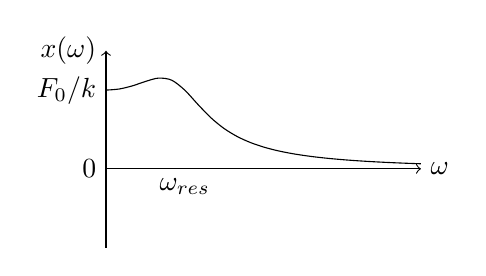
\begin{tikzpicture}
      \draw[->] (0,0) -- (4,0) node[right] {$\omega$};
      \draw[->] (0,-1) -- (0,1.5) node[left] {$x(\omega)$};
      \draw[domain=0:4,smooth,variable=\x,black] plot ({\x},{1/sqrt((1-\x^2)^2+\x^2});
      \draw (0,0) node[left]{0};
      \draw (0,1) node[left]{$F_0/k$};
      \draw (1,0) node[below]{$\omega_{res}$};
\end{tikzpicture}
\hspace{0.01cm}
\begin{tikzpicture}
      \draw[->] (0,0) -- (6,0) node[right] {$\omega$};
      \draw[->] (0,-1) -- (0,1.5) node[left] {$v(\omega)$};
      \draw[domain=0.01:6,smooth,variable=\x,black] plot ({\x},{1/sqrt((1-\x^2)^2/\x^2+1});
      \draw (0,0) node[left]{0};
      \draw (1,0) node[below]{$\omega_0$};
\end{tikzpicture}
\hspace{0.01cm}
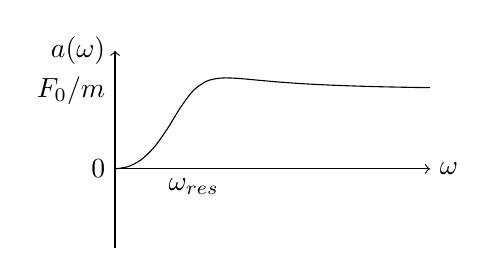
\begin{tikzpicture}
      \draw[->] (0,0) -- (4,0) node[right] {$\omega$};
      \draw[->] (0,-1) -- (0,1.5) node[left] {$a(\omega)$};
      \draw[domain=0:4,smooth,variable=\x,black] plot ({\x},{\x^2/sqrt((1-\x^2)^2+\x^2});
      \draw (0,0) node[left]{0};
      \draw (0,1) node[left]{$F_0/m$};
      \draw (1,0) node[below]{$\omega_{res}$};
\end{tikzpicture}
\end{center}
\item $|A(\omega)|=\frac{F_0/m}{\sqrt{(\omega_0^2-\omega^2)^2+\gamma^2\omega^2}}$ and $\delta=\tan^{-1}(\frac{-\gamma\omega}{\omega_0^2-\omega^2})$ For $\omega=30$, $|A|=0.0192$ and $\delta=180-16.7=163.3$\degree. For $\omega=20$, $|A|=0.1$ and $\delta=90$\degree. For $\omega=0$, $|A|=0.025$ and $\delta=0$\degree.
\item $P(\omega)=\frac{\gamma\omega^2(F_0^2/m)}{2((\omega_0^2-\omega^2)^2+\gamma^2\omega^2)}$ and $P(30)=0.165$ W, $P(20)=2.0$ W.
\end{enumerate}
\end{ans}
\newpage
\begin{qns}[Forced Damping and Square Wave]
A driving force $F(t) = F_1(t) + F_2(t)$ is applied to a damped oscillator, where $F_1(t) =\text{Re}[A_1e^{i\omega_1t}]$ and $F_2(t)=\text{Re}[A_2e^{i\omega_2t}]$. Show that, if $\omega_1\neq\omega_2$, the mean power absorbed by the system is given by $\langle P\rangle=\langle P_1\rangle+\langle P_2\rangle$ where $\langle P_1\rangle$ and $\langle P_2\rangle$ are the mean powers absorbed if only $F_1$ or only $F_2$ were applied respectively. What happens if $\omega_1=\omega_2$? Consider now an external force having the form of a square wave, which may be approximated as
$$F(t)=A_0\bigg(\sin\omega t+\frac{1}{3}\sin(3\omega t)+\frac{1}{5}\sin(5\omega t)\bigg)$$
Sketch the power absorption as a function of the angular frequency $\omega$ of the fundamental, if the oscillator has $\omega_0=$ 15 rad/s and $Q = 30$.
\end{qns}
\begin{ans}
Since we are applying to the same damped oscillator with mechanical impedance $Z_m$, we have
$$P_i=F_i\cos(\omega_it)\frac{F_i}{Z_m}\cos(\omega_it-\phi)\implies\langle P_i\rangle=\frac{F_i^2}{Z_mT}\int_0^T\cos^2(\omega_it)\cos\phi+\cos(\omega_it)\sin(\omega_it)\sin\phi dt=\frac{F_i^2}{2Z_m}\cos\phi$$
where $i=1,2$. But for $F=F_1+F_2$, the corresponding power is
$$P=(F_1\cos(\omega_1t)+F_2\cos(\omega_2t))\bigg(\frac{F_1}{Z_m}\cos(\omega_1t-\phi)+\frac{F_2}{Z_m}\cos(\omega_2t-\phi)\bigg)$$
Taking the time-averaged, we have $\langle P\rangle=\langle P_1\rangle+\langle P_2\rangle$ for $\omega_1\neq\omega_2$ since the time-averaged cross terms of different frequencies vanish. But for $\omega_1=\omega_2$, we have $\langle P\rangle=\langle P_1\rangle+\langle P_2\rangle+\frac{F_1F_2}{Z_m}\cos\phi$.\\[5pt]
Suppose the system achieve resonance at $\omega_0$, and the driving forces are of different frequencies $\omega_j$, then there will be resonance peaks at $\omega_j=\omega_0$ and of amplitude $\frac{F_j^2}{2Z_m}$. With the force $F(t)$, we naturally have 3 peaks for $P(\omega)$ against $\omega$ at $\omega=\omega_0$, $\omega=\omega_0/3$ and $\omega=\omega_0/5$ with ratios $1:1/9:1/25$ based on the form of $F(t)$. Note that $Q$ is the same for all 3 peaks ($Q$ is inherent to the system since the extent of damping is the same regardless of the force applied) and the corresponding half-power bandwidth is $\Delta\omega=\frac{\omega_0}{Q}$ for $\omega_0=15$ rad/s and is 0.5. Below is the sketch of the power spectrum where the finite bandwidth $(\Delta\omega=\omega_0/30)$ is not drawn. 
\begin{center}
\begin{tikzpicture}
      \draw[->] (0,0) -- (3,0) node[right] {$\omega$};
      \draw[->] (0,0) -- (0,5) node[left] {$P(\omega)$};
      \draw[blue] (0.5,0) -- (0.5,0.5);
      \draw[red] (1,0) -- (1,1);
      \draw[black] (2,0) -- (2,4);
      \draw (0,0) node[left]{0};
      \draw (0,0.5) node[left]{$1/25$};
      \draw (0,1) node[left]{$1/9$};
      \draw (0,4) node[left]{$1$};
      \draw (0.5,0) node[below]{$\frac{\omega_0}{5}$};
      \draw (1,0) node[below]{$\frac{\omega_0}{3}$};
      \draw (2,0) node[below]{$\omega_0$};
\end{tikzpicture}
\end{center}
\end{ans}
\newpage
\begin{qns}[Forced]
A simple pendulum whose damping is negligible oscillates freely with angular velocity $\omega_0$. A small horizontal force $F\sin\omega t$ is applied to the bob which has mass $m$.
\begin{enumerate}[label=(\alph*)]
    \item Show that the displacement $x$ of the bob follows
    $$\ddot{x}+\omega_0^2x=\frac{F}{m}\sin\omega t$$
    \item By considering the steady state response (the particular integral) and the free response (the complementary function), obtain the general solution of the above equation.
    \item If, at $t = 0$, the bob is at rest in its equilibrium position, show that
    $$x=\frac{F}{m(\omega_0^2-\omega^2)}\bigg(\sin\omega t-\frac{\omega}{\omega_0}\sin(\omega_0t)\bigg)$$
    Sketch a graph of this response as a function of time for the case $\omega=2\omega_0$.
    \item Without detailed calculation, discuss and sketch a graph of what happens if the damping is
small but not negligible.
\end{enumerate}
\end{qns}
\begin{ans}\leavevmode
\begin{enumerate}[label=(\alph*)]
\item The equation of motion is $m\ddot{x}+kx=F\sin\omega t$, with $k/m=\omega_0^2$.
\item The free response is $x(t)=c_1\sin(\omega_0t)+c_2\cos(\omega_0t)$. The steady state response is $\frac{F}{m(\omega_0^2-\omega^2)}\sin\omega t$, which is obtained by guessing a similar form for the particular solution. The general solution is a linear combination of both responses.
\item We guess a solution $x(t)=\frac{F}{m(\omega_0^2-\omega^2)}\sin(\omega t)+c_1\sin\omega_0t+c_2\cos\omega_0t$. Set $t=0$ for $\dot{x}$, we have $c_1=-\frac{\omega}{\omega_0}\frac{F}{m(\omega_0^2-\omega^2)}$. If $x(t=0)=0$, then $c_2=0$, and we obtain our desired solution. For $\omega=2\omega_0$, we have $\frac{2F}{3m\omega_0^2}\sin\omega_0t(1-\cos\omega_0t)$.
\begin{center}
\begin{tikzpicture}
      \draw[->] (0,0) -- (13,0) node[right] {$t$};
      \draw[->] (0,-1) -- (0,1.5) node[left] {$x(t)$};
      \draw[domain=0:12,smooth,variable=\x,black] plot ({\x},{-sin(\x*180/pi)*(cos(\x*180/pi)-1)});
      \draw (0,0) node[left]{0};
\end{tikzpicture}
\end{center}
\item If there is light damping present:
\begin{itemize}
    \item natural frequency is slightly reduced;
    \item transient term decays exponentially until eventually, only the driven response survives;
    \item magnitude of driven response falls slightly while a small phase shift is acquired between the driving force and the response.
\end{itemize}
\end{enumerate}
\end{ans}
\newpage
\begin{qns}[Computational Problem for Anharmonic]
A simple pendulum consists of a small bob of mass $m$ hanging
from a massless string of length $l$ in a gravitational field $g$. Its equation of motion is
$$\ddot{\theta}=-\frac{g}{l}\sin\theta$$
The pendulum is displaced by an angle $\theta_0$ and released from rest. Write a program to plot the displacement $\theta$ as a function of time for a few periods, for initial values $\theta_0=0.01, 0.03,0.1,1.0,2.0,3.0$ radians and comment on the results. (Assume for simplicity $g=10m/s^2$ and $l = 10m$. You may find it helpful to plot the normalised displacements, $\theta/\theta_0$, against time.). [Do not assume that the displacement is small. Using MATLAB to solve the differential equation, you
will need to rewrite it as two coupled first order equations in new variables $y_0=\theta$, $y_1=\dot{\theta}$ Then
use the routine ode45 to integrate the system. You may need to ensure the solution is sufficiently
accurate by setting the tolerance parameters appropriately e.g. something like odeset(’RelTol’,
1e-6);]
\end{qns}
\begin{ans}
As $\theta_0$ increases, the period gets slightly longer and the $\theta(t)$ profile deviates away from the usual sinusoidal form. In particular, the phase plot ($\dot{\theta}$ against $\theta$) is perturbed away from the usual circle.
\begin{figure}[H]
    \centering
    \includegraphics[width=\linewidth]{2_7.png}
    \caption{Amplitude profile and phase plot for $\theta_0=3.0$ radians for both harmonic and anharmonic case. (Plotted on Mathematica)}
\end{figure}
\end{ans}
\newpage
\subsection{Waves}
\begin{qns}[Transverse Pulse]
A uniform inextensible string of length $l$ and mass $m$ is suspended vertically. It is tapped at the top end so that a transverse pulse runs down it. At the same instant, a small body is released from rest at the top of the string, so that it falls freely parallel to the string.
\begin{enumerate}[label=(\alph*)]
    \item How far from the top of the string does the falling body catch up with the impulse?
    \item What mass should be hung from the string so that the pulse and the falling body reach the bottom simultaneously?
\end{enumerate}
\end{qns}
\begin{ans}\leavevmode
\begin{enumerate}[label=(\alph*)]
\item The velocity of propagation of transverse wave at point $x$ along the string is
$$v=\sqrt{\frac{T(x)}{\mu}}=\sqrt{\frac{(l-x)\mu g}{\mu}}=\sqrt{(l-x)g}$$
The time taken by the wave to traverse a distance $dx$ at this point is $dx/v$, and so
$$\delta t(x)=\int_0^x\frac{dx}{\sqrt{(l-x)g}}=\frac{2}{\sqrt{g}}[\sqrt{l}-\sqrt{l-x}]$$
But for the free-falling body, $\delta t(x)=\sqrt{2x/g}$. To see the position where they catch up, square them and we have
$$\sqrt{\frac{x}{2}}=\sqrt{l}-\sqrt{l-x}\implies x=0\text{ (NA)   },\frac{8}{9}l$$
\item Now the velocity is
$$v=\sqrt{\frac{T(x)}{\mu}}=\sqrt{\frac{(l-x)\mu g+Mg}{\mu}}$$
$$\implies\delta t(x)=\frac{1}{\sqrt{g}}\int_0^x\frac{dx}{\sqrt{(l-x)+(M/\mu)}}=\frac{2}{\sqrt{g}}[\sqrt{l+(M/\mu)}-\sqrt{l+(M/\mu)-x}]$$
when $x=l$, $\delta t(l)=(2/\sqrt{g})[\sqrt{l+(M/\mu)}-\sqrt{M/\mu}]$. we compare with $\sqrt{\frac{2l}{g}}$ again, then we have $-\frac{1}{4}=\frac{M}{m}-\sqrt{\frac{M}{m}}\sqrt{1+\frac{M}{m}}\implies\frac{m}{M}=8$, where $\mu=m/l$.
\end{enumerate}
\end{ans}
\newpage
\begin{qns}[Piano String Waves]\leavevmode
\begin{enumerate}[label=(\alph*)]
\item A steel piano string has a diameter of 0.5mm and a length of 700mm. The steel has a density of $\rho$= 7800 kgm$^{-3}$ and a Young’s modulus of $Y$ = 200GPa. What tension does the string have to be put under to tune the string to middle C (261.6 Hz)? High-strength steel has a yield strength of about $3\times10^9N/m^2$. Comment on the dangers of piano tuning.
\item What is the frequency of the fundamental longitudinal oscillation of this string?
\item With a few exceptions, most solids break if they are stretched by more than 1-2 \% of their unstretched length. Use this fact to show that transverse waves on a stretched string are almost always slower than compression waves on the same string.
\end{enumerate}
\end{qns}
\begin{ans}\leavevmode
\begin{enumerate}[label=(\alph*)]
\item We have the frequency of the transverse oscillation to be $$261.6=f=\frac{v}{\lambda}=\frac{1}{2L}\sqrt{T/(\rho A)}=\frac{1}{2(700\times10^{-3})}\sqrt{T/(7800\times\pi(0.5\times10^{-3}/2)^2)}\implies T=205.4 N$$ where $\mu=\rho A$ (density per unit length), $\lambda=2L$ (fundamental) with $L$ being the length of the string. This tension corresponds to a pressure of $\frac{T}{A}=\frac{205.4}{(0.5\times10^{-3}/2)^2}=1.05\times10^9N/m^2$, which is of the same order as magnitude of the yield strength. For higher frequencies, the tension needed to tune might result in pressure within the string to be greater than the yield strength, hence snapping the string.
\item The frequency of the fundamental longitudinal oscillation is $$f_L=\frac{1}{2L}\sqrt{Y/\rho}=\frac{1}{2(0.7)}\sqrt{\frac{200\times10^9}{7800}}=3620 Hz$$
\item The longitudinal velocity is 
$$v_{long}=\sqrt{Y/\rho}=\sqrt{\frac{T/A}{(\Delta L/L_0)/(m/LA)}}=\sqrt{\frac{(L_0/\Delta L)T}{m/L}}=\sqrt{\frac{L_0}{\Delta L}}v_{trans}$$
where $v_{trans}=\sqrt{T/(m/L)}=\sqrt{T/\rho A}$. Take say 2 \% change in length, then $v_{long}=\sqrt{50}v_{trans}$. Transverse waves are thus almost always slower than longitudinal waves, i.e. $\frac{v_{trans}}{v_{long}}=\frac{1}{\sqrt{50}}$. 
\end{enumerate}
\end{ans}
\newpage
\begin{qns}[Polarization]
Three transverse waves propagating in the $z$ direction have the following displacements in the $x$ direction:
\begin{enumerate}
    \item A wave which is linearly polarized at an angle $\theta$ to the $x$ axis with
    $$\Psi_{x,1}=a\cos\theta\cos(kz-\omega t+\phi_0)$$
    \item A right-circularly polarized wave (optical convention—looking into the source) with
    $$\Psi_{x,2}=b\cos(kz-\omega t)$$
    \item A right-elliptically polarized wave with
    $$\Psi_{x,3}=c\cos(kz-\omega t)$$
    (the major axis of the ellipse is twice the length of the minor axis and lies along the x axis).
\end{enumerate}
\begin{enumerate}[label=(\alph*)]
    \item Write down the corresponding displacements in the $y$ direction for each of these waves.
    \item An elliptically polarized wave can be produced by the superposition of the circularly polarized wave and the linearly polarized wave. Show that this is true for the waves given above for appropriate values of $\theta$, $\phi_0$, $a$ and $b$; find these values (you may assume $0\leq\theta\leq\pi/2$, $0\leq\phi_0\leq\pi/2)$. Draw vector diagrams in the $x$-$y$ plane showing the relationship between the displacements produced by the three waves at (i) $z = 0$, $t = 0$, (ii) $z = 0$, $\omega t =\pi/4$, (iii) $z = 0$, $\omega t = \pi/2$ and (iv) $kz = \pi/4$, $t = 0$. 
\end{enumerate}
\end{qns}
\begin{ans}\leavevmode
\begin{enumerate}[label=(\alph*)]
\item Since the first wave is linearly polarized, $\Psi_{y,1}=a\sin\theta\cos(kz-\omega t+\phi_0)$. For elliptical waves, we take $\sin$ instead of $\cos$, i.e. $\Psi_{y,2}=b\sin(kz-\omega t)$. In addition, for the third one, we take $c/2$ since it is given that the minor axis is half of the major axis, i.e. $\Psi_{y,3}=\frac{c}{2}\sin(kz-\omega t)$.
\item We have to find $a,b,\theta,\phi_0$ such that
$$a\cos\theta\cos(kz-\omega t+\phi_0)+b\cos(kz-\omega t)=c\cos(kz-\omega t)$$
$$a\sin\theta\cos(kz-\omega t+\phi_0)+b\sin(kz-\omega t)=0.5c\sin(kz-\omega t)$$
\begin{enumerate}[label=(\roman*)]
\item $z=0$, $t=0$:
$$a\cos\theta\cos(\phi_0)+b\cos(0)=c\cos(0)$$
$$a\sin\theta\cos(\phi_0)=0$$
this requires $\sin\theta=0\implies\theta=0$. Then, $a\cos\phi_0+b=c$. Let $\phi_0=0$, then $a=b=c/2$. The vectors are $\Psi_1=a(1,0)$, $\Psi_2=b(1,0)$, $\Psi_3=c(1,0)$.
\item $z=0$, $\omega t=\frac{\pi}{4}$:
$$a\cos\theta\cos\bigg(-\frac{\pi}{4}+\phi_0\bigg)+b\cos\bigg(-\frac{\pi}{4}\bigg)=c\cos\bigg(-\frac{\pi}{4}\bigg)\implies a\cos\theta\cos\bigg(-\frac{\pi}{4}+\phi_0\bigg)+b\frac{1}{\sqrt{2}}=c\frac{1}{\sqrt{2}}$$
$$a\sin\theta\cos\bigg(-\frac{\pi}{4}+\phi_0\bigg)+b\sin\bigg(-\frac{\pi}{4}\bigg)=0.5c\sin\bigg(-\frac{\pi}{4}\bigg)\implies a\sin\theta\cos\bigg(-\frac{\pi}{4}+\phi_0\bigg)-b\frac{1}{\sqrt{2}}=-c\frac{1}{2\sqrt{2}}$$
For the equations to be consistent, we have $\sin\theta=1\implies\theta=\frac{\pi}{2}$ and $\cos(-0.25\pi+\phi_0)=\frac{1}{\sqrt{2}}$ and hence $\phi_0=\frac{\pi}{2}$. Also have $a=0.5c$ and $b=c$. The vectors are $\Psi_1=(a/\sqrt{2})(0,1)$, $\Psi_2=(b/\sqrt{2})(1,-1)$ and $\Psi_3=(c/\sqrt{2})(1,-0.5)$. 
\item $z=0$, $\omega t=\frac{\pi}{2}$:
$$a\cos\theta\cos\bigg(-\frac{\pi}{2}+\phi_0\bigg)+b\cos\bigg(-\frac{\pi}{2}\bigg)=c\cos\bigg(-\frac{\pi}{2}\bigg)\implies a\cos\theta\cos\bigg(-\frac{\pi}{2}+\phi_0\bigg)=0$$
$$a\sin\theta\cos\bigg(-\frac{\pi}{2}+\phi_0\bigg)+b\sin\bigg(-\frac{\pi}{2}\bigg)=0.5c\sin\bigg(-\frac{\pi}{2}\bigg)\implies a\sin\theta\cos\bigg(-\frac{\pi}{2}+\phi_0\bigg)-b=-\frac{1}{2}c$$
We have $\sin\theta=1\implies\theta=\frac{\pi}{2}$ and $\cos(-0.5\pi+\phi_0)=1\implies\phi_0=0.5\pi$. So, $a=c/2=b/2$. The vectors are $\Psi_1=a(0,1)$, $\Psi_2=b(0,-1)$ and $\Psi_3=c(0,-0.5)$.
\item $kz=\frac{\pi}{4}$, $t=0$:
$$a\cos\theta\cos\bigg(\frac{\pi}{4}+\phi_0\bigg)+b\cos\bigg(\frac{\pi}{4}\bigg)=c\cos\bigg(\frac{\pi}{4}\bigg)\implies a\cos\theta\cos\bigg(\frac{\pi}{4}+\phi_0\bigg)+\frac{b}{\sqrt{2}}=\frac{c}{\sqrt{2}}$$
$$a\sin\theta\cos\bigg(\frac{\pi}{4}+\phi_0\bigg)+b\sin\bigg(\frac{\pi}{4}\bigg)=0.5c\sin\bigg(\frac{\pi}{4}\bigg)\implies a\sin\theta\cos\bigg(\frac{\pi}{4}+\phi_0\bigg)+\frac{b}{\sqrt{2}}=\frac{c}{2\sqrt{2}}$$
For the equations to be consistent, $\cos\theta=0\implies\theta=\frac{\pi}{2}$, then $\phi_0=0$, and $a=-c/2=-b/2$. The vectors are $\Psi_1=(a/\sqrt{2})(0,1)$, $\Psi_2=(b/\sqrt{2})(1,1)$ and $\Psi_3=(c/\sqrt{2})(1,0.5)$. 
\end{enumerate}
\end{enumerate}
\end{ans}
\begin{qns}[String Sinusodial Travelling]
A sinusoidal wave given by   $\psi=\text{Re}[Ce^{i(\omega t-kz)}]$ is travelling along a string of impedance $Z$, where $C$ is complex and $Z$ is real. Given that the instantaneous power transmitted by a travelling wave is given by $P(t)=Z(\frac{\partial\psi}{\partial t})^2$, show that the average power passing a given point in the string is given by $\langle P\rangle=\frac{1}{2}Z\omega^2|C|^2$. How would you interpret a complex value for $Z$ of $Z(\omega)$ at a given angular frequency $\omega$, and what would be the average power transmitted in this case?
\end{qns}
\begin{ans}
We have $\frac{\partial\psi}{\partial t}=\text{Re}[i\omega |C|e^{i(\omega t-kz+\phi)}]=-|C|\omega\sin(\omega t-kz+\phi)$, where $C=|C|e^{i\phi}$ then
$$P(t)=Z|C|^2\omega^2\sin^2(\omega t-kz+\phi)\implies \langle P\rangle=\frac{1}{2}Z\omega^2|C|^2$$
For complex $Z$, we have
$$\langle P\rangle=\frac{1}{2}\text{Re}[(Zv)^*v]=\frac{1}{2}|v|^2\text{Re}[Z]$$
Only the real part of $Z$ creates power flow along the wave system. The imaginary part of $Z$ generates a velocity response which is $\frac{\pi}{2}$ out of phase with the force, so that no energy on average is transmitted.
\end{ans}
\begin{qns}[Transverse Wave]
A string has mass per unit length $\mu$ and tension $T$. One end is free to move transversely but is attached to a massless vane which moves in a viscous fluid and therefore experiences a drag force of $\alpha u_v$ where $u_v$ is its transverse velocity. Show that if $\alpha$ is very small or very large, the wave is totally reflected. Is a node or an anti-node produced at the free end? What value of $\alpha$ leads to perfect absorption?\\[5pt]
A harmonic wave travels along the string towards the end attached to the vane. For a general value of $\alpha$, superposition of the incident and reflected waves gives rise to a combination of a standing wave and a travelling wave, no point on the string having zero amplitude. Show that for $\alpha<\sqrt{T\mu}$ the standing wave ratio, i.e. the ratio of the maximum amplitude to the minimum amplitude, is given by $\sqrt{T\mu}/\alpha$. Sketch the displacement of the string when the free end has (i) its maximum displacement and (ii) zero displacement, indicating the positions of the points of maximum and minimum amplitude. (Measuring the standing wave ratio is a convenient way of finding the impedance of a termination.)
\end{qns}
\newpage
\begin{ans}
We treat the end attached to the massless vane to be a medium of impedance $Z_2=\frac{\alpha u_v}{u_v}=\alpha$, while the string has impedance $Z_1=\sqrt{T\mu}$. The free end is not constrained, hence an anti-node. At the boundary between the two medium, the reflection coefficient is $r=\frac{Z_2-Z_1}{Z_2+Z_1}$.\\[5pt]
If $\alpha<<1$, $$r=-\frac{1-(Z_2/Z_1)}{1+(Z_2/Z_1)}\approx -1$$ which is a total reflection with a phase shift $\frac{\pi}{2}$ radians. If $\alpha>>1$, $$r=\frac{1-(Z_1/Z_2)}{1+(Z_1/Z_2)}\approx 1$$
which is a total reflection. For $r=0$ (perfect absorption), $Z_1=Z_2\implies\alpha=\sqrt{T\mu}$.\\[5pt]
For $\alpha<\sqrt{T\mu}$, we have $\frac{Z_2}{Z_1}<1$, which means $r=-\frac{1-(Z_2/Z_1)}{1+(Z_2/Z_1)}<0$. The partially reflected wave has a phase shift, leading to partial cancellation at points of minimum amplitude and add at points of maximum amplitude. The total wave looks like
$$\psi=\text{Re}[\psi_0e^{-i\omega t}(e^{ikx}+re^{-ikx})]=\text{Re}[\psi_0e^{-i\omega t}[(1-r)e^{ikx}+2r\cos(kx)]]$$
where $(1-r)e^{ikx}$ is a travelling wave term and $2r\cos(kx)$ is a standing wave term. The standing wave ratio is the ratio of the maximum to minimum amplitude for this resultant wave, which is $$\frac{1-r}{1-r+2r}=\frac{1-r}{1+r}=\frac{Z_1}{Z_2}=\frac{\sqrt{T\mu}}{\alpha}$$ where $r<0$.
\begin{enumerate}[label=(\roman*)]
\item When the free end is at maximum displacement, say $t=0$, then we let $\psi_{total}=\psi_0(1-r)\cos(kx)$, $\psi_t=\psi_0(1+r)\cos(kx)$ and $\psi_s=-\psi_02r\cos(kx)$.
\item When the free end is at zero displacement, say $t=\frac{\pi}{2\omega}$, then $$\psi_{total}=\psi_t=(1-r)\psi_0\sin(kx)$$ and $\psi_s=0$.
\end{enumerate}
\end{ans}
\newpage
\begin{qns}[Longitudinal Pressure Wave]\leavevmode
\begin{enumerate}[label=(\alph*)]
\item By considering the appropriate continuity conditions, derive from first principles the pressure amplitude reflection coefficient for a sound wave passing from a liquid of impedance $Z_1$ into a fluid of impedance $Z_2$. (You may assume normal incidence on a plane boundary.) What is the corresponding amplitude reflection coefficient?
\item Figure 1a shows apparatus in which a pulse of high-frequency sound is launched upwards through water by a transducer. In Figure 1b the feature labelled A shows the initial excitation of the transducer and B shows the arrival of the sound pulse back at the transducer after it has been reflected from the water-air interface. Calculate the velocity of sound, the acoustic impedance and the bulk modulus for water.
\begin{figure}[H]
    \centering
    \includegraphics[width=\linewidth]{2_13i.PNG}
\end{figure}
\item Figure 2a shows a similar experiment in which the water has the same depth but a thick layer of oil has been floated onto the water surface. Identify the pulses marked C and D in figure 2b. Calculate the velocity of sound and hence the acoustic impedance $Z_2$ for the oil.
\item Explain why pulse C in Figure 2b is smaller than pulse B in Figure 1b. Use the relative sizes of these pulses to test the formula derived in (a) for the reflection of sound at the water-oil interface. Does this result need correction for divergence or absorption of the sound beam?
\end{enumerate}
[Densities: water 1000 kgm$^{-3}$; the oil 790 kgm$^{-3}$ Acoustic impedance of air = 400 kgm$^{-2}$ s$^{-1}$]
\begin{figure}[H]
    \centering
    \includegraphics[width=\linewidth]{2_13ii.PNG}
\end{figure}
\end{qns}
\newpage
\begin{ans}\leavevmode
\begin{enumerate}[label=(\alph*)]
\item When a sound wave meets a boundary separating two media of different acoustic impedance., there are two boundary conditions that must be met physically to ensure the two media are in complete contact everywhere across the boundary:
\begin{itemize}
    \item Particle Velocity is continuous across the boundary;
    $$v_i+v_r=v_t$$
    \item Acoustic Excess Pressure is continuous across the boundary
    $$p_i+p_r=p_t$$
\end{itemize}
We have $p_i=\rho_1c_1v_i$, $p_r=\rho_1c_1(-v_r)$ and $p_t=\rho_2c_2v_t$, and also $Z=\rho c$. Hence, 
$$Z_1*(v_i-v_r)=Z_2*v_t=Z_2*(v_i+v_r)\implies\frac{v_r}{v_i}=\frac{Z_1-Z_2}{Z_1+Z_2}$$
Upon integrating can get $\frac{x_r}{x_i}$, the amplitude reflection coefficient for displacement, i.e. $\frac{x_r}{x_i}=\frac{Z_1-Z_2}{Z_1+Z_2}$. Also, we have $Z_1(-v_t+2v_i)=Z_2v_t\implies\frac{v_t}{v_i}=\frac{2Z_1}{Z_1+Z_2}$, which upon integrating is the amplitude transmission coefficient for displacement, i.e. $\frac{x_t}{x_i}=\frac{2Z_1}{Z_1+Z_2}$. For pressure, we have
$$\frac{p_r}{p_i}=\frac{\rho_1c_1}{\rho_1c_1}\frac{v_r}{v_i}=\frac{Z_1-Z_2}{Z_1+Z_2}$$
$$\frac{p_t}{p_i}=\frac{\rho_2c_2}{\rho_1c_1}\frac{v_t}{v_i}=\frac{Z_2}{Z_1}\frac{2Z_1}{Z_1+Z_2}=\frac{2Z_2}{Z_1+Z_2}$$
\item We take the time difference of pulse A and B (which is also the time difference between reflected and incident pulse to reach the transducer) is 83 $\mu$s. The pulse travels $2\times 63$ mm of distance. The velocity of wave in water is $c=\frac{2\times 63\times10^{-3}}{83\times10^{-6}}=1518$ m/s. The acoustic impedance for water is $Z=\rho c=1000\times 1518=1.518\times10^6$ kg m$^{-2}$ s$^{-1}$. The bulk modulus $B=Zc=2.30\times10^9$ Pa.
\item C is the pulse reflected from water-oil interface while D is that reflected from air-oil interface. It takes 20 $\mu$ s to travel 34 mm of oil, hence velocity in oil is $c=\frac{34\times10^{-3}}{20\times10^{-6}}=1700$ m/s. Also, the acoustic impedance of oil is $Z=\rho c=790\times1700=1.34\times10^6$ kg m$^{-2}$ s$^{-1}$.
\item Pulse C is the pulse reflected from the water-oil interface while B is the pulse reflected from the water-air interface. The difference in impedance between water and air is greater than that of water and oil, hence B should have a stronger pulse. 
$$\frac{1.52+1.34}{1.52-1.34}\approx 16=4^2$$
as expected, assuming the $y$-axis is the intensity, hence squaring the reflection coefficient.
\end{enumerate}
\end{ans}
\newpage
\begin{qns}[Longitudinal Pressure Wave]\leavevmode
\begin{enumerate}[label=(\alph*)]
\item A plane sinusoidal sound wave of displacement amplitude $1.2\times10^{-3}$ mm and frequency 680 Hz is propagated in a gas of density 1.3 kgm$^{-3}$ and pressure $1.0\times10^5$ Nm$^{-2}$ The ratio of principal specific heat capacities ($\gamma$) is 1.4. Find the pressure amplitude of the wave.
\item What frequency is heard if a thin steel bar of length 1.0 m is tapped on the end so as to launch a longitudinal wave pulse? What fraction of the pulse energy is lost into air each time the pulse reaches the end of the bar? Assuming this is the only mechanism of energy loss, calculate a characteristic decay time for the ringing of the bar.
\end{enumerate}
[The Young’s modulus of steel is 210GPa
and the density 7800 kgm$^{-3}$. The density of air is 1.2 kg m$^{-3}$ and the speed of sound in air is 340ms$^{-1}$.]
\end{qns}
\begin{ans}\leavevmode
\begin{enumerate}[label=(\alph*)]
\item The pressure amplitude is $$\Psi_{p,0}=\gamma pka_0=\frac{\gamma 2\pi fpa_0}{\sqrt{\gamma p/\rho}}=a_02\pi f\sqrt{\gamma p\rho}=(1.2\times10^{-6})2\pi(680)\sqrt{1.4\times 1.3\times(1.0\times10^5)}=2.2\text{Pa}$$
\item The frequency of the longitudinal wave pulse is
$$f=\frac{v}{\lambda}=\frac{\sqrt{Y/\rho}}{2L}=\frac{1}{2}\sqrt{\frac{210\times10^9}{7800}}=2600 Hz$$
The impedance of air is $\rho c=1.2\times 340=408$ kg m$^{-2}$ s$^{-1}$, while the impedance of steel is $\sqrt{Y\rho}=\sqrt{210\times10^9\times 7800}=4.05\times10^7$ kg m$^{-2}$ s$^{-1}$. The transmitted ratio for intensity is
$$\tau=\frac{4Z_{air}Z_{steel}}{(Z_{air}+Z_{steel})^2}=\frac{4\times 408\times 4.05\times10^7}{(4.05\times10^7+408)^2}=4.03\times10^{-5}$$
The time it takes for the pulse to travel across the 1 m steel bar is $\delta t=L/v=L/\sqrt{Y/\rho}$ and so to find the characteristic decay time:
$$(1-\tau)^N=e^{-1}\implies T=N\delta t=-\frac{1}{\ln(1-\tau)}L\sqrt{\frac{\rho}{Y}}=-\frac{1}{\ln(1-4.03\times10^{-5})}(1)\sqrt{\frac{7800}{210\times10^9}}=4.78s$$
\end{enumerate}
\end{ans}
\newpage
\begin{qns}[Computational Question]
A plane wave of unit amplitude, $e^{i(\omega t-k_1x)}$ propagates in the $+x$ direction of a region of impedance $Z_1$ which fills the region $x < 0$. It is incident normally on a layer of material of thickness $l$ and impedance $Z_2$ which fills the region $0 < x < l$. Some of it is in general reflected, so that the total disturbance in $x < 0$ is
$$\psi_1=e^{i(\omega t-k_1x)}+re^{i(\omega t+k_1x)}$$
where $r$ is the complex amplitude of the reflected wave. In steady state, region 2 in general contains forward and backward travelling waves of complex amplitudes $a$ and $b$:
$$\psi_2=ae^{i(\omega t-k_2x)}+be^{i(\omega t+k_2x)}$$
The layer lies on an infinite substrate of impedance $Z_3$, which fills the region $x > l$. In this region, the transmitted wave can be written
$$\psi_3=\tau e^{i(\omega t-k_3(x-l))}$$
for some complex transmitted amplitude $\tau$ . Note that $k_1$, $k_2$, $k_3$ are the wavenumbers in the three regions. Show that the boundary conditions at $x = 0$ and $x = l$ can be written in the form
$$\begin{pmatrix}-1&1&1&0\\1&Z_1/Z_2&-Z_1/Z_2&0\\0&e^{-ik_2l}&e^{ik_2l}&-1\\0&e^{-ik_2l}&-e^{ik_2l}&-Z_2/Z_3\\\end{pmatrix}\begin{pmatrix}r\\a\\b\\\tau\\\end{pmatrix}=\begin{pmatrix}1\\1\\0\\0\\\end{pmatrix}$$
Using MATLAB (or another language, perhaps Python), write a function which solves this matrix equation, taking as arguments the values $Z_1$, $Z_2$, $Z_3$, $k_2$ and $l$, and returning the vector of complex amplitudes $(r,a,b,\tau)$. Hence plot the amplitude and phase of the reflection ($r$) and transmission ($t$) coefficients as a function of thickness $l$ in the range 0 to 1 m for the cases
\begin{itemize}
    \item $k_2=2\pi$ m$^{-1}$, $Z_1=1\Omega$, $Z_2=2\Omega$, $Z_3=4\Omega$
    \item $k_2=2\pi$ m$^{-1}$, $Z_1=1\Omega$, $Z_2=3\Omega$, $Z_3=4\Omega$
\end{itemize}
To get the correct form of the equations, assume that for this wave system, for a wave of amplitude $\psi$, the
quantities $\psi$ and $\psi/Z$ are continuous ($Z$ is the impedance). Recall that the impedance for a wave traveling in the negative direction is $-Z$ The continuity equations at $x = 0$ are then $(1 + r) = (a + b)$ and $(1-r)/Z_1=(a-b)/Z_2$. 
\end{qns}
\begin{ans}
Imposing continuity conditions for $\psi$ at $x=0$ and $x=l$ respectively gives
$$1+r=a+b$$
$$ae^{-ik_2l}+be^{ik_2l}=\tau$$
Imposing continuity conditions for $\psi/Z$ at $x=0$ and $x=l$ respectively gives
$$\frac{1-r}{Z_1}=\frac{a-b}{Z_2}$$
$$\frac{ae^{-ik_2l}-be^{ik_2l}}{Z_2}=\frac{\tau}{Z_3}$$
After rearranging, we obtain the desired matrix. Plotting on Mathematica:
\begin{figure}[H]
    \centering
    \includegraphics[width=\linewidth]{2_15a.PNG}
    \caption{$Z_2=2\Omega$}
\end{figure}
\begin{figure}[H]
    \centering
    \includegraphics[width=\linewidth]{2_15b.PNG}
    \caption{$Z_2=3\Omega$}
\end{figure}
Observe that $|r|=0$ for $l=0.25$ and $l=0.75$. Also, there is better impedance matching for $Z_2=\sqrt{Z_1Z_3}=2\Omega$, as desired.
\end{ans}
\newpage
\begin{qns}[Reflection]
A long string (extending from $x\in(-\infty,\infty)$) with mass per unit length $\mu$ = 0.2 kgm$^{-1}$ lies on a smooth horizontal table, and is put under uniform tension. A point mass $m$ = 0.005 kg is attached to the string at $x = 0$. A wave of wavelength $\lambda$ = 0.1m propagates along the string, in the plane of the table, from $x=-\infty$ and strikes the mass.
\begin{enumerate}[label=(\alph*)]
    \item What fraction of energy is reflected by the mass?
    \item Where should another identical mass be attached so as to eliminate the reflection?
\end{enumerate}
\end{qns}
\begin{ans}\leavevmode
\begin{enumerate}[label=(\alph*)]
\item We have two regions, left and right of the point mass with the same impedance $Z$. Guess a form
$$\psi=Ae^{i(kx-\omega t)}+Are^{-i(kx+\omega t)};\text{  }A\tau e^{i(kx-\omega t)}$$
for region I and II separately. $k$ is the same for both regions since $\mu$ and $Z$ are the same. The boundary condition $\psi$ being continuous at $x=0$, still holds:
$$1+r=\tau$$
But the boundary condition for $T\psi'$ is now discontinuous at $x=0$, allowing the mass to accelerate, i.e. $m\frac{\partial^2\psi}{\partial t^2}=T[\frac{\partial\psi}{\partial x}]_I^{II}$, which is Newton's second law:
$$-m\omega^2A\tau=TikA(\tau-(1-r))$$
Rearranging, we have $r=-\frac{1}{1+2ikT}{m\omega^2}$. Bear in mind that $T=\mu v^2$ and so $\frac{4k^2T^2}{\omega^4}=\frac{4\mu^2}{k^2}$, so
$$|r|^2=\frac{1}{1+\frac{4k^2T^2}{m^2\omega^4}}=\frac{1}{1+\frac{\mu^2\lambda^2}{m^2\pi^2}}=\frac{1}{1+\frac{0.2^20.1^2}{(0.005)^2\pi^2}}=0.382$$
38.2 \% of the energy is reflected by the mass.
\item We have three regions, I, II and III such that the ansatz for the three regions are $\{Ae^{i(kx-\omega t)}+rAe^{-ikx-i\omega t}\}$, $\{Aae^{i(kx-\omega t)}+Abe^{-ikx-i\omega t}\}$ and $\{A\tau e^{i(kx-\omega t)}\}$ respectively. The boundary condition $\psi$ being continuous at $x=0$ and $x=l$ yield respectively:
$$1+r=a+b$$
$$a+be^{-2ikl}=\tau$$
The discontinuity condition for $T\psi'$ at $x=0$ and $x=l$, is Newton's second law, which gives
$$\frac{ikm}{\mu}(1+r)=a-b-1+r$$
$$\frac{ikm}{\mu}\tau=\tau-a+be^{-2ikl}$$
where we used $\frac{k}{\mu}=\frac{\omega^2}{Tk}$. We aim to find $l$ such that $r=0$. Using a change of variables, by setting $\gamma:=e^{-ikl}$ and $\beta:=\frac{m\omega^2}{kT}=\frac{mk}{\mu}=\frac{0.005}{0.2}\frac{2\pi}{0.1}=\frac{\pi}{2}$. 
\begin{equation}
    a+b=1\tag{E1}
\end{equation}
\begin{equation}
    a+b\gamma^2=\tau\tag{E2}
\end{equation}
\begin{equation}
    a-b-1=i\frac{\pi}{2}\tag{E3}
\end{equation}
\begin{equation}
    -a+b\gamma^2=i\tau\frac{\pi}{2}-\tau\tag{E4}
\end{equation}
Add E1 and E3 to get $2a-1=1+i\frac{\pi}{2}\implies a=1+i\frac{\pi}{4}$ and hence $b=-i\frac{\pi}{4}$. Thus, $\tau=a+b\gamma^2$, and so E4 gives
$$\gamma^2=\frac{i0.5\pi a}{2b-i0.5\pi b}=\frac{i0.5\pi(1+i0.25\pi)}{-i0.5\pi-0.5\pi0.25\pi}=\frac{\frac{\pi^2}{16}-1}{\frac{\pi^2}{16}+1}-i\frac{\frac{\pi}{2}}{\frac{\pi^2}{16}+1}$$
The argument of $\gamma=e^{-ikl}$ gives $-kl$. To find this, the argument of $\gamma^2$ is $-\pi-\tan^{-1}(\frac{\pi/2}{(\pi^2/16)-1})=-1.81$ rad. But, the argument of $\gamma^2$ is twice of that of $\gamma$, and so $-ikl=-0.905\implies l=\frac{0.905}{2\pi/0.1}=14.4$ mm.
\end{enumerate}
\end{ans}
\begin{qns}[Dispersive Water Waves]\leavevmode
\begin{enumerate}[label=(\alph*)]
\item Show that the group velocity $v_g$ can be written as
$$v_g=v_p-\lambda\frac{dv_p}{d\lambda}$$
where $v_p$ is the phase velocity and $\lambda$ the wavelength of the disturbance. The phase velocity for surface waves in a liquid of depth $>>\lambda$ is given by
$$v_p=\sqrt{\frac{g\lambda}{2\pi}+\frac{2\pi\sigma}{\rho\lambda}}$$
where $\sigma$ is the surface tension and $\rho$ is the density. Find an expression for the group velocity. Hence show that in the long wavelength limit, when gravity dominates,
$$v_g=0.5v_p$$
A disturbance of frequency 1 Hz occurs on the surface of a deep lake. How long will it take the resulting wave group to reach a point 1km distant?
\item Storms in the Pacific ocean with sustained strong winds cause swells (groups of gravity-driven waves) which can create great surfing conditions when they arrive on California’s beaches. A surfer in California notes that the group of waves she is surfing has a typical wave period of 18 s. Twenty-four hours later, she goes surfing again and notices the period is now 17 s. Explain this phenomenon, and estimate the distance to the storm, and the windspeed in the storm.
\end{enumerate}
\end{qns}
\begin{ans}\leavevmode
\begin{enumerate}[label=(\alph*)]
\item We evaluate $\frac{dv_p}{d\lambda}$:
$$\frac{dv_p}{d\lambda}=\frac{1}{k}\frac{dk}{d\lambda}\bigg(\frac{d\omega}{dk}-v_p\bigg)$$
with $dk/d\lambda=-2\pi/\lambda^2$. Since $v_g=\frac{d\omega}{dk}$, we obtain our desired relation. We have $v_p^2=\frac{g\lambda}{2\pi}+\frac{2\pi\sigma}{\rho\lambda}$, then
$$\lambda\frac{dv_p}{d\lambda}=\bigg(\frac{g\lambda}{2\pi}-\frac{2\pi\sigma}{\rho\lambda}\bigg)\frac{1}{2v_p}\implies v_g=v_p-\lambda\frac{dv_p}{d\lambda}=\frac{2v_p^2-(\frac{g\lambda}{2\pi}-\frac{2\pi\sigma}{\rho\lambda})}{2v_p}\approx\frac{g\lambda}{2\pi}\frac{1}{2}\sqrt{\frac{2\pi}{g\lambda}}$$
where in the long wavelength limit, $\lim_{\lambda\rightarrow\infty}v_p=\sqrt{\frac{g\lambda}{2\pi}}$, then $v_g$ in this limit is $\frac{1}{2}v_p$.\\[5pt]
Recall definition of phase velocity, $v_p=\frac{\omega}{k}=f\lambda$ and so $\lambda=\frac{v_p}{f}$. In the long wavelength limit, we have $v_p^2\approx\frac{g\lambda}{2\pi}=\frac{g}{2\pi}\frac{v_p}{f}\implies v_p=\frac{g}{2\pi f}\implies v_g=\frac{g}{4\pi f}$. The time taken is 1 km divided by $v_g$ which is 1280 s.
\item The distance is equal to $v_g(\tau=18s)T$ and also equal to $v_g(\tau=17s)(T+1\text{day})$ where $\tau$ is the period $1/f$ of the wave while $T$ is the time taken it takes for the wave to reach from the source to the receiver. Longer period waves travel faster.\\[5pt]
We had $v_g=\frac{g}{4\pi f}=\frac{g\tau}{4\pi}$. So,
$$\frac{g\tau}{4\pi}T=\frac{g(\tau-1)}{4\pi}(T+24\times 3600)\implies 1=\bigg(1-\frac{1}{\tau}\bigg)\bigg(1+\frac{24\times 3600}{T}\bigg)$$
which gives $T=1.4688\times10^6$s and so the distance is $\frac{g\times 18}{4\pi}\times T$ to be $2.06\times10^7$ m. To find the windspeed of the storm. we observe its phase speed, i.e. $v_p=2v_g=\frac{2(9.81)(18)}{4\pi}\approx28$ m/s.
\end{enumerate}
\end{ans}
\newpage
\begin{qns}[Dispersive EM Waves]
Discuss what is meant by group velocity and phase velocity, and distinguish between dispersive and non-dispersive media. For electromagnetic waves of frequency $f$ in a dispersive medium of refractive index $n$, the frequency dependent phase velocity is given by $c/n$, where $c$ is the speed of light in a vacuum. Denoting the group velocity $u_g$, show that
$$\frac{c}{u_g}=n+f\frac{dn}{df}$$
A communication system uses square pulses of infrared radiation transmitted along optical fibres. The infrared laser has a frequency of $f_0=2.0\times10^{14}$ Hz, and each pulse has a duration $T_P=1.0\times10^{-10}s$. The refractive index of the fibres in this frequency range is given by
$$n(f)=n_0+\tau(f-f_0)$$
where $\tau=10^{-16}$s and $n_0=1.5$. The time interval between successive pulses is $T_R=10^{-9}$s.
\begin{enumerate}[label=(\alph*)]
    \item Sketch the power spectrum of the signal, and estimate the range of frequencies present in the signal.
    \item Find the group velocity at the centre frequency $\nu_0$ and estimate the range of group velocities present in each pulse.
    \item Explain why the pulses spread out as they travel along the fibre. Estimate the maximum length of fibre that can be used without the pulses running into each other (neglecting waveguide dispersion).
\end{enumerate}
\end{qns}
\begin{ans}
Dispersive waves have the following dispersion relation: $\omega(k)$ that is not a constant, and is a function of $k$. Different wavelengths travel at different phase speeds. The phase velocity of a wave is the rate at which the phase of the wave propagates in space. This is the velocity at which the phase of any one frequency component of the wave travels, i.e. any harmonic wave: $v_p=\frac{\omega(k)}{k}$. The group velocity of a wave is the velocity of the interference maximum of a wavepacket. $v_g=\frac{\partial\omega(k)}{\partial k}|_{k=k_0}$ For a dispersive wave, $v_g\neq v_p$. In a non-dispersive media, the waves do not exhibit a dispersion relation.\\[5pt]
We have $ck=n\omega$ for electromagnetic waves. Hence, 
$$c\frac{\partial k}{\partial\omega}=n+\omega\frac{\partial n}{\partial\omega}\implies\frac{c}{u_g}=n+2\pi f\frac{\partial n}{\partial(2\pi f)}=n+f\frac{dn}{df}$$
\begin{enumerate}[label=(\alph*)]
\item In the time domain, the signal $g(t)$ consists of a sine wave of frequency $f_0=2\times10^{14}$ Hz, multiplied by a top hat function of width $T_P=10^{-10}$ s (duration of pulse). This is then convolved with an infinite comb of delta functions with spacing $T_R=10^{-9}$ s (time interval between successive pulses). The Fourier transform of this signal $\tilde{g}(f)$ is:\\[5pt]
The carrier sine wave transforms to a delta function at $f_0$ (as well as a negative delta function at $-f_0$ if the oscillation is a sine wave). The top hat transforms to a sinc function $\frac{\sin(\pi fT_P)}{\pi fT_P}$. This sinc function has a zero at $\Delta f=\frac{1}{T_P}=10$ GHz, and another one at $-\Delta f$. When we convolve this sinc function with the delta function, it shifts it to be centred at $f_0$ with zeros at $f_0\pm \Delta f$. Finally, we multiply by the Fourier transform of the comb function (finely-spaced infinite comb of delta functions with spacing $\frac{1}{T_R}=1$ GHz). \\[5pt]
Essentially, the sketch is a comb modulated by a sinc envelope. The central peak has a full width at half maximum power of about $\Delta f=10$ GHz, hence the signal contains frequencies $(f_0\pm\frac{\Delta f}{2})=(2\times10^{14}\pm 5\times10^9)$ Hz.
\item 
$$n(f)=1.5+10^{-16}(f-2\times10^{14})$$
$$\frac{c}{u_g}=1.5+\tau(f-f_0)+f\tau=1.5+\tau(2f-f_0)\implies u_g=\frac{3\times10^8}{1.5+10^{-16}((2-1)2\times10^{14})}=1.97\times10^8 m/s$$
For $f_0\pm\Delta f$,
$$\Delta u_g=\frac{\partial u_g}{\partial f}\Delta f=-\frac{2\tau c}{(1.5+\tau(2f_0-f_0))^2}\Delta f\implies|\Delta u_g|=\frac{2(10^{-16})(3\times10^8)10^{10}}{(1.5+10^{-16}\times2\times10^{14})^2}=260m/s$$
So the group velocity is $(1.97\times10^8\pm 130)$ m/s.
\item The refractive index of the fibres result in the velocity of the wavepacket to be frequency dependent. As the wavepacket travels, the range of group speeds present cause the wavepacket to disperse. We have the distance to be $v_g(fast)T=v_g(slow)(T+T_R)$ and so
$$\frac{1.97\times10^8+130}{1.97\times10^8-130}=1+\frac{T_R}{T}$$
The distance is $(1.97\times10^8-130)T$ which gives $1.49\times10^5$ m.
\end{enumerate}
\end{ans}
\begin{qns}[Computational]\leavevmode
\begin{enumerate}[label=(\alph*)]
\item A particular wavepacket can represented by a sum of travelling waves with different amplitudes, all with wavevectors close in magnitude to the central wavevector $k_0$:
$$\psi(x,t)=\sum_{m=-m_0}^{m_0}e^{-(k_m-k_0)^2}{2\sigma_k^2}\cos(k_mx-\omega(k_m)t)$$
The dispersion relation $\omega (k)$ for this wavesystem is
$$\omega(k) = ck + dk^3$$
and the wavevector of the $m$-th component is $k_m=k_0+m\Delta k$.\\[5pt] 
Using the values $k_0$ = 1 m$^{-1}$ (i.e. a central wavelength of $2\pi$m), $\sigma_k=k_0/10$, $\Delta k=\sigma_k/10$, $c = 1m/s$, d = 0 (i.e. no dispersion), $m_0$ = 30, use MATLAB (or another language) to calculate and plot the disturbance at times $t$ = 0 s, 100 s, 200 s and 300 s.\\[5pt]
Repeat the plots with differing amounts of dispersion (e.g. $d=\pm0.2m^3s^{-1}$, $d=\pm0.1m^3s^{-1}$) and describe the results qualitatively, and where possible quantitatively. In particular, discuss the speed at the which the packet propagates, and the rate at which is spreads.
\item A travelling square wave can be modelled as a Fourier series:
$$\psi(x,t)=\cos[k_0x-\omega(k_0)t]-\frac{1}{3}\cos[3k_0x-\omega(3k_0)t]+\frac{1}{5}\cos[5k_0x-\omega(5k_0)t]+...$$
or, truncating after $m_0+1$ terms, we have
$$\psi(x,t)\approx\sum_{m=0}^{m_0}\frac{(-1)^m}{2m+1}\cos[k_mx-\omega(k_m)t]$$
The dispersion relation $\omega(k)$ for this system is taken to be $\omega=ck+dk^3$, and the wavevector of the $m$'th component wave is $k_m=(2m+1)k_0$.\\[5pt] 
Using the values $k_0=1$ m$^{-1}$, $c=1$ m s$^{-1}$, $d=0$ (i.e. no dispersion), $m_0=10$, use MATLAB or otherwise to calculate and plot the disturbance at times $t=0$, $t=\pi$ s, $t=2\pi$ s.\\[5pt]
Repeat the plots with differing amounts of dispersion ($d=0.001$ m$^3$ s$^{-1}$, $-0.001$ m$^3$ s$^{-1}$, 0.02 m$^3$ s$^{-1}$ and 0.05 m$^3$ s$^{-1}$) and describe the results qualitatively, and where possible quantiatively.\\[5pt]
Explain how these results relate to the design of digital communication systems.
\end{enumerate}
\end{qns}
\begin{ans}
The problem is coded in Mathematica and the figures are in the next two pages. Dispersion $d\neq 0$ will result in the square wave to be distorted, affecting the transmission of square waves (and most other waves) in communication.
\end{ans}
\begin{figure}[H]
    \centering
    \includegraphics[width=\linewidth]{19a.pdf}
    \caption{19a: (first row) $d=0$, (second row left) $d=0.1$, (second row right) $d=-0.1$, (third row left) $d=0.2$, (third row right) $d=-0.2$;}
\end{figure}
\begin{figure}[H]
    \centering
    \includegraphics[width=\linewidth]{19b.pdf}
    \caption{19b: (first row) $d=0$, (second row left) $d=0.001$, (second row right) $d=-0.001$, (third row left) $d=0.002$, (third row right) $d=0.05$;}
\end{figure}
\newpage
\begin{qns}[Evanescent Waves]
A transmission line, such as a coaxial cable, consists of two conductors, and is used to carry electrical signals. The voltage $V(x,t)$ along such a cable lying on the $x$-axis obeys the equation
$$\frac{\partial^2V}{\partial x^2}=LC\frac{\partial^2V}{\partial t^2}+RC\frac{\partial V}{\partial t}$$
where $R,C,L$ are the resistance, capacitance and inductance per unit length of the cable respectively. A sinusoidal voltage of angular frequency $\omega$ is applied at the end $x = 0$ of a very long cable, resulting in a travelling wave $V(x,t)=V_0e^{i(kx-\omega t)}$ Assuming that the resistance per unit length $R$ is small
$(R<<\omega L)$, find expressions for (i) the wavevector $k$, and (ii) the phase speed of the signal. Show that the signal is attenuated as it propagates, and find an expression for the attenuation length (the length over which the signal amplitude falls by a factor e).
\end{qns}
\begin{ans}
Using the suggested solution, we have 
$$-k^2V_0=LC(-\omega^2V_0)+RCi\omega V_0\implies k^2=\omega^2LC\bigg(1+\frac{iR}{\omega L}\bigg)$$
$$\implies k=\pm\omega\sqrt{LC}\sqrt{1+\frac{iR}{\omega L}}\approx\pm\omega\sqrt{LC}\bigg(1+\frac{iR}{2\omega L}\bigg)=\pm\omega\sqrt{LC}\pm i\frac{R}{2}\sqrt{\frac{C}{L}}$$
We have $V(x,t)=V_0e^{i(kx-\omega t)}=V_0e^{-(R/2)\sqrt{C/L}x}e^{i(\omega\sqrt{LC}x-\omega t)}$. The phase speed is $\frac{\omega}{\omega\sqrt{LC}}=\frac{1}{\sqrt{LC}}$. The decay length is where the amplitude decays to $1/e$ of its initial value, and this is thus $\frac{2}{R}\sqrt{\frac{L}{C}}$.
\end{ans}
\begin{qns}[Standing Wave]
Two plane waves are represented by
$$\Psi_1=e^{-i(k_xx+k_yy)},\Psi_2=e^{-i(k_xx-k_yy)}$$
Note the term $e^{i\omega t}$ have been omitted from the representation.
\begin{enumerate}[label=(\alph*)]
    \item Show that the result of superposing these disturbances is a wave travelling in the positive $x$ direction with amplitude $A = 2\cos(k_yy)$.
    \item Show that $l$, the spacing of the nodal lines in the $y$ direction, is given by $l=\pi/k_y$.
    \item By substituting into the wave equation show that $k_x^2+k_y^2=\omega^2/u^2$, where $u$ is the speed of the waves.
    \item A rubber sheet is fastened to rigid supports along two lines parallel to the $x$ axis so as to make a waveguide. The width of the guide is 0.1 m. In the absence of the supports the speed of waves on the sheet is 2 m/s. For waves of frequency 12 Hz, calculate the phase velocity and group velocity for propagation along the guide. What happens to waves of frequency 8 Hz? Sketch the instantaneous displacement of the membrane in a section of the guide at (i) 12 Hz and (ii) 8 Hz.
\end{enumerate}
\end{qns}
\begin{ans}\leavevmode
\begin{enumerate}[label=(\alph*)]
\item We have $\Psi_1+\Psi_2=e^{-ik_xx}(e^{-ik_yy}+e^{+ik_yy})=e^{-ik_xx}2A\cos(k_yy)$, a standing wave of amplitude $2\cos(k_yy)$.
\item For this resultant ampltiude to be zero, we require $y=\frac{(m+0.5)\pi}{k_y}$, $m\in\mathbb{Z}$ and so the spacings of the nodal lines are $\Delta y=l=\frac{\pi}{k_y}$.
\item The 2D wave equation is $\frac{\partial^2}{\partial x^2}+\frac{\partial^2}{\partial y^2}=\frac{1}{u^2}\frac{\partial^2}{\partial t^2}$. The second derivative of the time component on the right will give $\omega^2$ while the second derivative of the space component gives $k_x^2+k_y^2$. This gives $v^2=\frac{\omega^2}{k_x^2+\frac{n^2\pi^2}{l^2}}$.
\item Here, $v=2m/s$, $b=0.1m$. The phase velocity is $v_p=\frac{\omega}{k_x}=\frac{\omega}{\sqrt{(\omega/v)^2-(n\pi/b)^2}}$. This gives the cut-off frequency to be $\frac{1}{2\pi}\frac{\pi nv}{b}=10n$ Hz. Any frequencies below this cut-off frequency will give imaginary $k_x$ and hence evanescent waves. $\forall n$, waves of frequency 8Hz do not propagate and will attenuate as evanescent wave. For $f=12$ Hz, we consider $n=1$, then $v_p=\frac{2\pi f}{\sqrt{(\omega/v)^2-(n\pi/b)^2}}=3.62$ m/s, and $v_g=\frac{v^2}{v_p}=1.11$ m/s. Also, $\frac{2\pi}{k_1}=\frac{2\pi}{\sqrt{(2\pi f/v)^2-(\pi/b)^2}}=0.3m$. One thus plot the 2D contour plot for
\begin{enumerate}[label=(\roman*)]
\item 12 Hz: $\sin(\frac{\pi}{0.1}y)\sin(2\pi 12 t-\sqrt{(2\pi 12/2)^2-(\pi /0.1)^2}x)$ 
\item 8 Hz: $\sin(2\frac{\pi}{0.1}y)\sin(2\pi 8t)e^{-x\sqrt{(2\pi /0.1)^2-(2\pi 8/2)^2}}$, for two instances of time $t=0$ and $t=\frac{\pi}{2\omega}$.
\end{enumerate}
\end{enumerate}
\end{ans}
\subsection{Optics}
\begin{qns}[Diffraction and Interference for Two Slits]
An aperture consists of two long slits each of width $a$, with their centres separated by a distance $b$. The aperture is illuminated by a plane wave at normal incidence.
\begin{enumerate}[label=(\roman*)]
\item Show that the diffracted amplitude in direction $\theta$ for monochromatic illumination by light of wavelength $\lambda$ is directly proportional to 
$$2\psi_0a\cos(0.5kb\sin\theta)\sinc(0.5ka\sin\theta)$$
where $k=2\pi/\lambda$.
\item Show how your result can be derived from the Fourier transforms of a delta-function and a top-hat function. Describe with the aid of sketches how the Fourier transform changes with $a$ and $b$.
\item Show that the ratio of the width of the central peak of the envelope function to that of the central interference fringe is $2(b/a)$. (Note that this result is independent of $\lambda$.)
\item Derive the diffraction pattern above by treating the aperture as a superposition of a slit of width $b+a$ and a second slit of width $b-a$ the latter covered by a sheet of glass which inverts the phase of the light passing through it.
\end{enumerate}
\end{qns}
\begin{ans}\leavevmode
\begin{enumerate}[label=(\roman*)]
\item The diffracted amplitude is directly proportional to
$$\psi_0\int_{b/2-a/2}^{b/2+a/2}e^{-iqx}dx+\int_{-b/2-a/2}^{-b/2+a/2}e^{-iqx}dx=\frac{\psi_0}{iq}(e^{-iqb/2}+e^{iqb/2})2\sin\frac{qa}{2}=\frac{4a\psi_0}{i}\cos(qb/2)\sinc(qa/2)$$
hence directly proportional to $2\psi_0a\cos(kb\sin\theta/2)\sinc(ka\sin\theta/2)$.
\item Let $h_1(x)$ be a top-hat function of width $a$,
$$\tilde{h}_1(q)=\int_{-a/2}^{a/2}e^{iqx}dq=\frac{a}{2}\frac{2\sin(qa/2)}{qa/2}=a\sinc(qa/2)$$
Let $h_2(x)$ be $\delta(x+b/2)+\delta(x-b/2)$,
$$\tilde{h}_2(q)=\int_{-\infty}^\infty[\delta(x-b/2)+\delta(x+b/2)]e^{-iqx}dx=2\cos(qb/2)$$
The aperture function is $h(x)=h_1(x)*h_2(x)$. We have $\psi$ to be directly proportional to $\mathcal{F}[h_1*h_2]=\tilde{h}_1(q)\tilde{h}_2(q)=2a\cos(qb/2)\sinc(qa/2)$, by the convolution theorem. As $a$, increases, the width of $\tilde{h}_2(q)$'s main lobe decreases. As $b$ increases, the period of $\tilde{h}_1(q)$ decreases.
\item The first zero of the interference peak occur at $\frac{\pi}{2}=\frac{qb}{2}$ (cosine function), and so the width of the interference fringe is $2q=2k\sin\theta=\frac{2\pi}{b}$. The first zero of the diffraction envelope occur at $\pi=\frac{qa}{2}$ (sinc function), and so the width of the diffraction envelope's central peak is $2q=2\frac{2\pi}{a}$. The ratio is thus $2b/a$.
\item We have $\psi(\theta)$ to be directly proportional to
$$\psi_0\int_{-(b+a)/2}^{(b+a)/2}e^{-iqx}dx+\psi_0\int_{-(b-a)/2}^{(b-a)/2}e^{i\pi}e^{-iqx}dx=\frac{\psi_0}{iq}\bigg[(e^{iqb/2}+e^{-iqb/2})(-e^{-iqa/2}+e^{iqa/2})\bigg]=\frac{\psi_0}{iq}2\cos\frac{bq}{2}2i\sin\frac{qa}{2}$$
which simplifies to $=2a\psi_0\cos(bq/2)\sinc(qa/2)$, as desired.
\end{enumerate}
\end{ans}
\newpage
\begin{qns}[Resolution]
A digital camera has a lens with a focal length $f$ which can varied between 14 mm and 150 mm. Light enters the lens via a circular iris diaphragm of variable diameter. The $f$-number of the lens, $N$, can be varied from $N = 4$ to $N = 32$ (The $f$-number is the ratio of the lens focal length to diameter of the circular aperture; an $f$-number of 4 is usually written $f=4$ etc). The image is focused onto a CCD detector of size 17.3 mm $\times$ 13.0 mm, which contains 16 million detectors (pixels), which can be assumed to be square with no spaces between them. Evaluate, as a function of $N$, whether the image quality is limited by diffraction or by the size of the detectors. (Assume a typical wavelength
of $\lambda$ = 600 nm.)
\end{qns}
\begin{ans}
The angular size of the Airy disc is $\theta=\sin^{-1}(1.22\frac{\lambda}{D})$. The spatial size of the Airy disc is $f\tan\theta\approx f\sin\theta=1.22\frac{f\lambda}{D}=1.22\lambda N$ and in metres, it is $7.32\times10^{-7}N$, as a function of $N$. The Airy disc is bigger than the length scale of a pixel if 
$$2\times 1.22\lambda N\geq\sqrt{\frac{17.3\times10^{-3}\times 13.6\times10^{-3}}{16\times10^6}}=3.7\mu m\implies N\geq 2.527$$
Indeed, the Airy disc is bigger than the pixel, since $N_{min}=4$. The minimum spatial size of the Airy disc is $58.5$ mm, which is larger than the length scale of the grid of pixels.
\end{ans}
\begin{qns}[Fraunhofer Diffraction]
Calculate and sketch the Fraunhofer diffraction patterns of the following apertures, using the conventional Fourier space coordinates $(p,q)=(k\sin\theta,k\sin\xi)$:
\begin{enumerate}[label=(\alph*)]
    \item an infinite chequerboard consisting of transparent and opaque squares, each of side $a$;
    \item a transparent square aperture (with sides of length $2a$) whose lower half ($|x|<a$, $y<0$) is covered by a sheet of transparent film which introduces a phase delay of $\pi/2$;
    \item a transparent elliptical aperture with major axis $2a$ and minor axis $2b$, the major axis being aligned with x axis (hint: scaling);
    \item an array of 6 very small, identical circles arranged in a regular hexagon whose sides are of length $a$, with 2 of the circles located at $(x_i, y_i) = (0,\pm 2a)$.
    \item The figure shows the Fraunhofer diffraction patterns of the letters C, E, and F, in unknown order: which is which?
\end{enumerate}
\begin{figure}[H]
    \centering
    \includegraphics[width=\linewidth]{2_24.PNG}
\end{figure}
\end{qns}
\newpage
\begin{ans} We define $\text{rect}(z)$ to be 1 for $z\leq\frac{1}{2}$ and 0 otherwise. For each part (other than part e), we find the exact expression for the aperture function $h$. Use convolution theory, if necessary, to find the Fourier transform of the aperture function $\tilde{h}$. The Fraunhofer diffraction pattern will be directly proportional to $|\tilde{h}|^2$.
\begin{enumerate}[label=(\alph*)]
\item We treat the chequerboard as an infinite lattice, consist of a grid of lattice points, with each lattice point being a repeating unit cell. Each unit cell will be a 2 by 2 subgrid, with two transparent squares along the 45\degree diagonal. The aperture function for this unit cell is
$$h_{unit}(x,y)=\text{rect}(x/a)\text{rect}(y/a)*[\delta(x)\delta(y)+\delta(x-\frac{a}{\sqrt{2}})\delta(y-\frac{a}{\sqrt{2}})]$$
Observe that adjacent unit cells are separated by a distance of $2a$ apart. The infinite 2D grid of delta functions has aperture function
$$h_{grid}(x,y)=\sum_{n=0}^\infty\sum_{m=0}^\infty\delta(x-m2a)\delta(y-n2a)$$
The chequerboard aperture function is the convolution of $h_{unit}$ and $h_{grid}$. By the convolution theorem, $\tilde{h}=\tilde{h}_{unit}\tilde{h}_{grid}$. $\tilde{h}_{unit}$ can be easily computed by looking along the diagonal line: $\tilde{h}_{unit}(p,q)=\cos(\frac{p+q}{\sqrt{2}}a)\sinc\frac{pa}{2}\sinc\frac{qa}{2}$. Finally, $\tilde{h}_{grid}(p,q)$ is basically $\sum_{n=0}^\infty\sum_{m=0}^\infty\delta(p-\frac{2\pi m}{2a})\delta(q-\frac{2\pi n}{2a})$. Hence, the intensity is directly proportional to 
$$\tilde{h}_{unit}(p,q)\tilde{h}_{grid}(p,q)=\cos\bigg(\frac{p+q}{\sqrt{2}}a\bigg)\sinc\frac{pa}{2}\sinc\frac{qa}{2}\bigg[\sum_{m=0}^\infty\sum_{n=0}^\infty\delta\bigg(p-\frac{\pi m}{a}\bigg)\delta\bigg(q-\frac{\pi n}{a}\bigg)\bigg]$$
\item We treat the square aperture as two horizontal rectangles, with the lower half possessing a phase delay of $\frac{\pi}{2}$. The aperture function is 
$$h(x,y)=\bigg(\text{rect}\frac{2x}{a}\times\text{rect}\frac{y}{a}\bigg)*[\delta(x-0.25a)+i\delta(x+0.25a)]$$
We have the Fourier transform of $\delta(x\pm0.25a)$ to be $e^{\pm ipa/4}$. Take out a factor of $e^{i\pi/4}$, we will get $\cos(0.25(pa+\pi))$. By convolution theorem again, $\tilde{h}$ is
$$\tilde{h}(p,q)=\sinc\frac{pa}{4}\sinc\frac{qa}{2} e^{i\pi/4}\cos\bigg(\frac{pa+\pi}{4}\bigg)$$
\item Consider a circular aperture of aperture function $h_{circle}(x,y)$, which equals to 1 if $x^2+y^2\leq1$ and zero otherwise. The corresponding intensity for the circular aperture is directly proportional to $(\frac{J_1(2\pi\sin\theta/\lambda)}{2\pi \sin\theta/\lambda})^2=(\frac{J_1(k\sin\theta)}{k\sin\theta})^2$. Here, we have rotational symmetry about the line perpendicular to the aperture plane. To generalize, we change it to $(\frac{J_1(\sqrt{k_x^2\sin^2\theta_x+k_y^2\sin^2\theta_y})}{\sqrt{k_x^2\sin^2\theta_x+k_y^2\sin^2\theta_y}})^2$.\\[5pt]
The aperture function of this elliptical aperture $h_{ellipse}(x,y)$ equals to 1 if $(x/a)^2+(y/b)^2<1$ and zero otherwise. Using a change of coordinates $x'=x/a$ and $y'=y/b$, we can ensure the elliptical integration region becomes circular again. Alternatively, given that the scaled version of the Fourier transform is
$$\tilde{h}(x/a,y/b)=\frac{1}{|ab|}\tilde{h}(pa,qb)$$
then we have the final intensity to be directly proportional to 
$$\bigg(\frac{J_1(\sqrt{a^2p^2+q^2b^2})}{\sqrt{a^2p^2+b^2q^2}}\bigg)^2$$
\item The aperture function is
$$h(x,y)=\bigg[\sum_{i=1}^6\delta(x-x_i)\delta(y-y_i)\bigg]*o(x,y)$$
where $(x_i,y_i)=(0,\pm2a)$, $(\sqrt{3}a,\pm a)$, $(-\sqrt{3}a,\pm a)$ for the hexagonal geometry and $o(x,y)$ is the aperture function for a single hole. Taking the Fourier transform, we have
$$F(p,q)=\int h(x,y)e^{i(px+qy)}dxdy=O(p,q)\bigg[(e^{i2aq}+e^{-i2aq})+e^{-\sqrt{3}pai}(e^{iaq}+e^{-iaq})+e^{\sqrt{3}pai}(e^{iaq}+e^{-iaq})\bigg]$$
where $O(p,q)=\mathcal{F}[o(x,y)]$. The intensity is thus directly proportional to $(2\cos(2qa)+4\cos(\sqrt{3}pa)\cos(qa))^2$.
\item  From left to right: F, C, E. Looking at the letters, we see that the C has 2 horizontal bars of vertical spacing, say $x$, while the E and F have each three and two horizontal bars respectively, with half the spacing $0.5 x$. For the spectrum:
\begin{itemize}
    \item C will have the finest horizontal pattern spacings;
    \item Both C and F will have double slit patterns along the horizontal;
    \item E will have a single subsidiary maximum between the main fringe peaks.
    \end{itemize}
\end{enumerate}
\end{ans}
\begin{qns}[Fraunhofer Diffraction]
The Fraunhofer diffraction patterns of the letters of the alphabet are presented below, in alphabetical order, with 4 letters missing. Which ones?
\begin{figure}[H]
    \centering
    \includegraphics[width=\linewidth]{2_25.PNG}
\end{figure}
\end{qns}
\begin{ans}
The official answer gave:
\begin{figure}[H]
    \centering
    \includegraphics[width=\linewidth]{2_25a.PNG}
    \caption{Actual diffraction patterns of the letters. Image credit: Official answers}
\end{figure}
We need to appeal to basic symmetry properties here. Furthermore, it helps to remember these Fraunhofer diffraction patterns:
\begin{itemize}
    \item An open circle gives a circular Airy pattern. so we expect an annulus to give the difference between two Airy patterns with different scale sizes;
    \item A single long line aperture gives a narrow line of light at right angles to the aperture line modulated by a $\sinc^2$ pattern. So any straight line elements making up a letter will each generate diffracted amplitude along a line orthogonal to that line element;
    \item A set of parallel line elements will give diffraction pattern of a grating.
\end{itemize}
Some obvious ones: B is D convolved by a pair of delta functions along the vertical, W is V convolved by a pair of delta functions along the horizontal. With some guesswork and symmetry arguments, the missing letters are U, E (or maybe F), N and J.
\end{ans}
\newpage
\begin{qns}[Diffraction Grating]
A diffraction grating has period $D$, and each element of the grating consists of a pair of long narrow slits separated by $D/N$ where $N$ is an integer.
\begin{enumerate}[label=(\alph*)]
\item Sketch the diffraction pattern when the grating is normally illuminated.
\item Calculate the relative intensities $I_n$ of the various diffraction peaks of order $n$ for the case $N = 4$. Which peaks are “forbidden”?
\item For the case $N = 2$ show that the solution reduces to that of a simple grating of period $D/2$.
\end{enumerate}
\end{qns}
\begin{ans}\leavevmode
\begin{enumerate}[label=(\alph*)]
\item Assume the grating spans to infinity, we can just convolve the pair of slits with delta functions, i.e.
$$\bigg\{\delta\bigg(x-\frac{D}{2N}\bigg)+\delta\bigg(x+\frac{D}{2N}\bigg)\bigg\}*\bigg[\sum_{n=-\infty}^\infty\delta(x-nD)\bigg]=2\cos\bigg(\frac{qD}{2N}\bigg)\sum_{n=-\infty}^\infty\delta\bigg(q-\frac{2n\pi}{D}\bigg)$$
\item To compute the forbidden peaks $n$th order for the Dirac comb, we require $\cos\frac{qD}{2N}=0\implies\frac{qD}{2N}=\frac{2m+1}{2}\pi$ for $m\in\mathbb{Z}\cup\{0\}$. $\frac{qD}{\pi}=(2m+1)N$. For $N=4$, the envelope is zero at $\frac{qD}{\pi}$ values of 4, 12, 20, 28,... This gives the forbidden peaks. Visible peaks occur at even integer values of $\frac{qD}{\pi}$.
\item For $N=2$, forbidden peaks occur at $\frac{qD}{\pi}$ values of 2, 6, 10, 14, ... Visible peaks occur for even integer values of $\frac{qD}{\pi}$ and so every other peak is missing. The period between even peaks are $\frac{2\pi}{D}\times 2=\frac{2\pi}{D/2}$. This pattern is identical to that of a simple grating of period $D/2$.
\end{enumerate}
\end{ans}
\begin{qns}[Line Broadening]\leavevmode
\begin{enumerate}[label=(\alph*)]
\item This plot shows the spectrum of the rotational emission line from carbon monoxide molecules in an interstellar gas cloud. The rest frequency of the transition is 115 GHz. Estimate the temperature of the cloud, assuming the linewidth is due to Doppler broadening.
\begin{figure}[H]
    \centering
    \includegraphics[scale=0.7]{2_27.PNG}
\end{figure}
\item Estimate the contribution to the linewidth caused by pressure broadening in such a cloud if the
density of the gas (assumed for simplicity to be pure carbon monoxide) is $10^9$m$^{-3}$ and that the cross section for collisions between molecules is $10^{-19}$m$^2$.
\end{enumerate}
\end{qns}
\begin{ans}\leavevmode
\begin{enumerate}[label=(\alph*)]
\item For the half-power points, i.e. $\frac{1}{2}=e^{-(27\times10^3)^2/2\sigma_f^2}$. From the graph, $\sigma-\sigma_f=27$ kHz. The temperature is $T=\frac{\sigma_f^2}{f_0^2}\frac{mc^2}{k_B}=(\frac{27\times10^3}{115\times10^9})^2\frac{4.48\times10^{-26}\times 9\times10^{16}}{1.38\times10^{-23}}=12$ K.
\item We use $u=\sqrt{3kT/m}=103.5$ m/s, then $\Delta f\sim nu\Sigma=10^9(103.5)(10^{-19})=1.04\times10^{-8}$ Hz.
\end{enumerate}
\end{ans}
\newpage
\begin{qns}[Fraunhofer Diffraction]
Describe how the Fraunhofer diffraction pattern of a grating depends on:
\begin{enumerate}[label=(\alph*)]
\item the spacing between the grating lines;
\item the overall extent of the grating;
\item the amplitude distribution over an individual line;
\item the phase distribution over an individual line.
\end{enumerate}
A grating with 2500 lines per metre, each line 100 $\mu$m wide, is illuminated at normal incidence with light of 600 nm wavelength. Each line is divided lengthwise into halves, one of which introduces an additional half wavelength of path. Sketch the form of the Fraunhofer diffraction pattern. Show that it is symmetrical about the centre and derive the intensities $I_n$ of the diffracted beams for order $n=0,\pm1,\pm2,\pm3$, expressed relative to $I_1$. How might the phase distribution of each line be further modified in order to increase preferentially the intensity of beams on one side of the pattern?
\end{qns}
\begin{ans}
For an aperture described by the aperture function $h(x)$, the Fraunhofer diffraction pattern is proportional to the square of the Fourier transform of $h(x)$, i.e.
$$\bigg|\int h(x) e^{-iqx}\bigg|^2$$
where $q=k\sin\theta$. For a diffraction grating of finite span of slits with finite widths, $h(x)$ is given by
$$h(x)=\bigg(\sum_{m=0}^\infty\delta(y-mD)*\text{rect}\frac{y}{a}\bigg)\times\text{rect}\frac{y}{b}$$
which is a convolution of a single slit top-hat function $\text{rect}\frac{y}{a}$ and an infinite span delta comb with separation intervals equal to the spacing between the slits, $D$, followed by a multiplication of another top-hat function to ensure the grating is finite. Surely, $b>a$, where $a$ is the width of each slit and $b$ is the length span of the grating. By the Convolution theorem, the Fourier transform of the aperture function is 
$$\mathcal{F}[h(x)]=\bigg(\sum_{m=0}^\infty\delta(q-m\frac{2\pi}{D})\times a\sinc\frac{qa}{2}\bigg)*b\sinc\frac{qb}{2}$$
The corresponding diffraction pattern is a sinc envelope (dependent on the width of each slit, $a$) and sinc peaks (dependent on the length span of the grating, $b$) separated by $\frac{2\pi}{D}$ in $q$-space, hence related to the slit separation $D$. Hence
\begin{enumerate}[label=(\alph*)]
    \item The spacing between the grating lines $D$ is inversely proportional to the separation between intensity peaks, $\frac{2\pi}{D}$;
    \item The width of the individual peaks is inversely proportional to the overall extent of the grating $b$.
    \item The amplitude distribution over an individual line is dependent on the wider sinc envelope, in turn affected by the width of each slit $a$. Changing the amplitude distribution over an individual line would involve the Fourier transform of the function $g(x)$ that represents this amplitude distribution over this individual line. 
    \item Varying the phase distribution over an individual line would involve translating the pattern of that corresponding line linearly, by an amount equal to this new phase shift.
\end{enumerate}
Now consider an individual slit of width $2a=100$ $\mu$m. To account for the additional half wavelength of path being introduced, the aperture function will be $h(x)=1$ for $x\in[-a,0]$ and $h(x)=-1$ for $x\in[0,a]$ and zero otherwise. Then,
$$\int_{-a}^0e^{-iqx}dx-\int_0^ae^{-iqx}dx=-\frac{2i}{q}(\cos(qa)-1)=\frac{4}{iq}\sin^2(qa/2)=a^2q\sinc^2(qa/2)$$
We assume the diffraction grating is infinitely long in extent. Then, by convolution theorem, the corresponding intensity $I_n(q)$ is directly proportional to
$$\bigg(\sum_{n=0}^\infty\delta(q-\frac{n2\pi}{D})\bigg)^2\sinc^2(qa/2)q$$
where $\frac{1}{d}=2500\implies d=400$ $\mu$m. Since we have $qa=2\pi$ and $qd=2\pi$, the number of peaks between two consecutive minima of the envelope is $\frac{2\pi/a}{2\pi/d}=\frac{d}{a}=8$.\\[5pt]
Since $\delta(-x)=\delta(x)$ and $\cos(x)=\cos(-x)$, we have $I_n(-q)=I_n(q)$, even symmetry about the centre. Due to the $\cos(qa)-1$ modulation, the intensity is zero at the centre, so the intensity of the zeroth order is zero, i.e. $\frac{I_0}{I_1}=0$. Trivially, $\frac{I_{\pm1}}{I_1}=1$ (by even symmetry). Lastly,
$$\frac{I_2}{I_1}=\bigg(\frac{\cos\frac{4\pi a}{d}-1}{\cos\frac{2\pi a}{d}-1}\bigg)^2\bigg(\frac{2\pi/d}{4\pi/d}\bigg)^2=\frac{1}{4}\bigg(\frac{\cos(\pi/2)-1}{\cos(\pi/4)-1}\bigg)^2\approx 2.91$$
$$\frac{I_3}{I_1}=\bigg(\frac{\cos\frac{6\pi a}{d}-1}{\cos\frac{2\pi a}{d}-1}\bigg)^2\bigg(\frac{2\pi/d}{6\pi/d}\bigg)^2=\frac{1}{9}\bigg(\frac{\cos(3\pi/4)-1}{\cos(\pi/4)-1}\bigg)^2\approx 3.77$$
To preferentially increase the intensity of the beams on one side of the pattern, we need a function $f(x)$ such that the Fourier transform of $h(x)e^{if(x)}$ (function representing a single slit), gives us a lop-sided shape about the vertical axis. For example, add a phase shift of $\pi$ on one half of each line. Alternatively, add a small prism to each slit (which acts like a linear phase gradient).
\end{ans}
\begin{qns}[Diffraction Grating]
What is meant by the resolution and order of the spectrum of a diffraction grating? It is
planned to resolve a pair of spectral lines of mean wavelength 656.3nm and separation 0.015nm, using a standard spectrometer configuration of spectral slit and collimator lens (100mm focal length) to produce a parallel beam of light which falls normally onto a plane diffraction grating (600 lines per mm); the diffracted beams are viewed with a telescope. What requirements does the required spectral resolution place on:
\begin{enumerate}[label=(\alph*)]
\item the size of the diffraction grating;
\item the diameters of the collimator and telescope objective lenses?
\end{enumerate}
\end{qns}
\begin{ans}
The resolution of a diffraction grating refers to our ability to distinguish two adjacent intensity peaks. The order of the spectrum is an index on the intensity peak measured with respect to a central peak that is usually indexed as the zeroth order.\\[5pt]
By Rayleigh's criterion, the peaks are just resolvable if one peak falls on the first minimum of the adjacent peak. The first minima of the $n$th peak can be found at
$$k\sin\theta=\frac{2\pi n}{D}+\frac{2\pi}{W}\implies\sin\theta=\frac{\lambda n}{D}+\frac{\lambda}{W}$$
where $D$ is the distance between slits and $W$ is the width of the grating. For the adjacent peak with $\lambda+\delta\lambda$,
$$\sin\theta=\frac{(\lambda+\delta\lambda)n}{D}$$
By the Rayleigh's criterion, this is equal to the previous result, which gives us
$$\frac{\lambda n}{D}+\frac{\lambda}{ W}\leq\frac{\lambda+\delta\lambda}{D}n\implies W\geq\frac{D}{n}\frac{\lambda}{\delta\lambda}$$
\begin{enumerate}[label=(\alph*)]
\item For $\lambda=656.3\times10^{-9}$ m, $\delta\lambda=0.015\times10^{-9}$ m, $D=\frac{1}{600}\times10^{-3}=1.67\times10^{-6}$ m, we have $W\geq\frac{10^{-3}}{600n}\frac{656.3}{0.015}=\frac{0.07292}{n}$ for $n\in\mathbb{Z}$.
\item We placed the collimator and the telescope at the conjugate points of the grating.
\end{enumerate}
\end{ans}

\newpage
\begin{qns}[Fresnel Edge]
Signals from a transmitter of 0.1 m wavelength situated at a height of 2 m above the ground are picked up by a receiver in a radio telescope 22 m above ground at a distance of 1 km. It is desired to screen the receiver from these signals by erecting an absorbing screen 50m from the transmitter. How high must it be if the received power is to be reduced by a factor of 100? (Neglect reflections from the ground.)
\end{qns}
\begin{ans}
For the received power to be reduced by a factor of 100, the amplitude must be reduced by 10. The original length is from the point (0.5,0.5) to the origin on the Cornu spiral, and this length is $\frac{1}{\sqrt{2}}$. So the desired point on the Cornu spiral is (0.55,0.45) such that
$$\frac{1}{10\sqrt{2}}=\sqrt{(0.5-0.55)^2+(0.5-0.45)^2}$$
On the Cornu spiral (in the notes), the interval $\delta w$ between each successive cross is $\delta=0.2$. There are about 11.6 of such intervals, which give us a value of $\Delta w=11.6\times 0.2=2.32$. But, $\Delta w=\Delta x\sqrt{\frac{2}{\lambda R}}$. We have $R$ to be the harmonic mean between source to wall and wall to receiver, i.e. $R=((1/50)+(1/950))^{-1}=47.5$ m. This gives $$2.32=\Delta x\sqrt{\frac{2}{0.1\times 47.5}}\implies \Delta x=3.6 m$$
$\Delta  x$ is the distance between the top of the screen and the light path. The height of the source with respect to ground level is 2 m. Together with the inclination of the path between source and receiver, there is an additional height of 1 m. The wall thus must cover up to a vertical distance of 3.6 m above this path. Hence, the wall has a total height of $1+2+3.6=6.6$ m.
\end{ans}
\begin{qns}
[Computational Exercise for Fresnel Diffraction]
An aperture lies in the $x$-$y$ plane at $z = 0$, and consists of a long slit of width $d$. The slit is transparent in the region $|y|<d/2$; elsewhere it blocks incoming light. It is illuminated at normal incidence by a plane wave of wavelength $\lambda$ travelling in the $z$ direction. The diffraction pattern is observed on a screen at $z=D$ parallel to the aperture.\\[5pt]
The complex diffraction pattern observed on the screen at coordinate $(0,Y,D)$ can be written in the approximate form $\psi(Y)$ is directly proportional to
$$\int_{-d/2}^{d/2}\exp(ikr)K(\theta)dy$$
where $k=2\pi/\lambda$, $r=\sqrt{(Y-y)^2+D^2}$, $\tan\theta=\frac{Y-y}{D}$ and $K(\theta)$ is the obliquity factor. Explain the origin of this equation in terms of Huygens’ construction.\\[5pt]
Use MATLAB (or another language) to compute the complex diffraction pattern $\psi(Y)$ by integration.
Use the values $\lambda =$ 500 nm, $d =$ 1 mm, and assume the obliquity factor is unity: $K(\theta)=$ 1. Plot the diffracted intensity $|\psi(Y)|^2$ for $D=$ 10 mm, 100 mm, 326 mm, 640 mm and 4000 mm and comment on the patterns as $D$ varies (recall the Fresnel distance is $d^2/\lambda$).\\[5pt]
[You will need to use a MATLAB integration routine such as quad or quadgk. You can check some of your patterns against Fig. 10.70 in Hecht’s Optics book.]
\end{qns}
\begin{ans}
Based on Huygen's Principle, the secondary wavelets emerge from each point on the primary wavefront and these secondary wavelets interfere with each other on the screen, based on the principle of superposition. The final wave at a point on the screen would then be given by the sum of wavefunctions from each secondary wavelet at the aperture. This sum hence takes the form of an integral, due to the need to add up infinitesimally small contributions from each secondary wavelet.\\[5pt]
$e^{ikr}$ represents the phase shift increment due to the wave travelling a path distance $r=\sqrt{(Y-y)^2+D^2}$ which is the distance from position $y$ at the aperture to position $Y$ on the screen (both points lie on the same $y$-$z$ plane $x=0$). $K(\theta)$ is the obliquity factor that ensures the wavefront does not backpropagate.\\[5pt]
The Fresnel distance is $D=\frac{d^2}{\lambda}=\frac{(1\times10^{-3})^2}{500\times10^{-9}}=2$ m. For $D=4000$ mm, it is the Fraunhofer regime since we see the usual sinc envelope modulating the peaks. Any value of $D$ below this, we have Fresnel diffraction.
\end{ans}
\newpage
\begin{figure}[H]
    \centering
    \includegraphics[width=\linewidth]{31.pdf}
    \caption{Plots of $|\psi(Y)|^2$ against $Y$, ignoring the proportionality constant. From left to right, then top to bottom are increasing $D$ values. Notice the length scale of $Y$ where most of the pattern appears increases with $D$. Also, the intensity $|\psi(Y)|^2$ increases with $D$. In particular, one sees a $\sinc$ envelope if $D$ is greater than the Fresnel distance, i.e. the Fraunhofer regime.}
\end{figure}
\newpage
\begin{qns}[Fresnel Edge]
While an observer on Earth is observing a distant star, the Moon moves across the observer’s line of sight, blocking out the star: this is a lunar occultation. The speed of the Moon relative to the Earth’s surface is 500m/s and the apparent velocity vector lies perpendicular to the edge of the moon that blocks the star. The star is being observed through a filter which transmits only a small
range of wavelengths near 500 nm and the Moon is 4$\times10^5$ km from the observer.
\begin{enumerate}[label=(\alph*)]
\item Sketch the apparent brightness of the star as a function of time (the ’lightcurve’) during the occultation, assuming the star is a point source of light. (You may assume that the limb of the moon acts as a straight edge).
\item What is the time between the last two maxima in brightness before the star disappears?
\item Explain how the observed light curve would change if the star’s angular size was not negligible.
\end{enumerate}
\end{qns}
\begin{ans}\leavevmode
\begin{enumerate}[label=(\alph*)]
\item We treat the limb of the Moon as a straight edge, a locally correct approximation. The distance between the Moon and the star is taken to be infinity, and so the harmonic mean of the source (star) to obstacle and the obstacle to screen (observer on Earth) is just $R=4\times10^8$ m.\\[5pt]
When the Moon is far away from the point source, the apparent brightness of the star is the same as when it is not blocked. As the Moon gradually approaches the star, there is sinusoidal albeit small (grow larger as the Moon approaches) variations of the brightness, until a maximum intensity of 138 \% is attained. When the Moon's straight edge is collinear with the observer and source, the brightness drops to 25 \%. Subsequently, the brightness decays off, but non-zero even after the Moon continues to obstruct it (can still `see' the star in the geometric shadow).
\item We take the maximum possible distance from (0,0) to any point on the Cornu spiral. On this point where the distance is maximum, $w_1=6\times 0.2$ (on the diagram in the notes, each interval between successive cross is $\delta w=0.2$). For the next maximum (after one revolution around the spiral), $w_2=11.5\times 0.2$. Hence, $\Delta w=(11.5-6)\times 0.2=11$. We thus have
$$11=\Delta w=\Delta h\sqrt{\frac{2}{\lambda R}}=\sqrt{\frac{2}{500\times10^{-9}\times 4\times10^8}}\implies\Delta h=110m$$
Hence, the time between last two maxima is $t=\frac{\Delta h}{v}=\frac{110}{500}=0.22$ s.
\item Convolve the sketch in part (a) with the brightness distribution of the star. One would expect the oscillatory behaviour to be washed out.
\end{enumerate}
\end{ans}
\begin{qns}[Fresnel Zones]
Plane waves of monochromatic ($\lambda$ = 0.5 $\mu$m) light are incident normally on an aperture. A
detector is situated on axis at a distance of $D = 20$ mm from the aperture plane.
\begin{enumerate}[label=(\alph*)]
    \item What is the value of $\rho_1$, the radius of the first Fresnel half-period zone on the aperture, as observed from the detector?
    \item If the aperture is a circular hole of radius $r$ = 1 mm, centred on axis, how many half-period zones does it contain? Sketch the intensity received by the detector if it were moved along the axis such that $D$ takes on values in the range ($20\pm 1$) mm. If the detector is moved away from the aperture along the optical axis, what is the furthest distance from the aperture that zero intensity will be detected?
    \item If the aperture is a zone plate with odd numbered zones blocked out, and with the radius of the first zone equal to $\rho_1$ as in (a), determine the first three focal lengths of the zone plate.
    \item If the detector is moved along the axis away from the aperture, what is the distance $D$ at which the final clear minimum is observed?
\end{enumerate}
\end{qns}
\newpage
\begin{ans}\leavevmode
\begin{enumerate}[label=(\alph*)]
\item Let the $n$th period zone have a radius $r_n$ on the plate, and $D=20$ mm be the distance to the detector. Then, $r_n=\sqrt{n\lambda D}$ where $r_1=\sqrt{\lambda D}=\sqrt{0.5\times10^{-6}\times 20\times10^{-3}}=100\mu$ m.
\item If the outer zone has radius $a=r_N=\sqrt{N\lambda D}1$ mm, then $N=\frac{a^2}{\lambda D}=100$. There is thus 100 half-period zones across the aperture. The intensity will be zero on the axis as odd and even zones cancel out (to first order). Varying $D$ will vary the number of half period zones. If this number is odd, you will get a maximum, so $D=(20.0\pm 0.2 j)$ mm where $j$ is odd, we have a maxima. Similarly, when $j$ is even, we have a minima.
\item The principal focus is $D=20$ mm. But $\frac{D}{3}$ and $\frac{D}{5}$ are foci as well. At those distances, the half-period zones defined at distance $D$ contain 3 and 5 half-period zones respectively. So the first three focal lengths are at 20 mm, 6.7 mm, 4 mm.
\item The final zero (minimum) occurs when the open disc subtends just two half period zones. $D'=\frac{a^2}{2\lambda}$. 
\end{enumerate}
\end{ans}
\begin{qns}[Poisson's Spot]
In an experiment to observe Poisson’s spot, a black circular disc is placed in front of, and orthogonal to, a plane wave light source of wavelength $\lambda=0.5\mu$m. The light falls onto a screen orthogonal to the incoming rays at a distance $D = 2.0$ m. The disc has a nominal radius of $r = 4.0$ mm, but manufacturing errors cause its radius to vary irregularly, with standard deviation $\pm\sigma$ from its nominal radius.\\[5pt]
For Poisson’s spot to be observed, how accurately circular must the disc be, i.e. what value of $\sigma$ can be tolerated? Give your answer in terms of the Fresnel half-period zones, and calculate its size in this example. Estimate the size of the bright spot in this example if the disc is perfectly circular. How is the argument for Poisson’s spot affected if the incident light is: (a) white; (b) not perfectly collimated (i.e. from an extended, incoherent source)?
\end{qns}
\begin{ans}
Recall the near-circular phasor diagram for Fresnel diffraction with a circular obstacle at the centre. Phasors slowly spirals into the centre as the upper limit of integration becomes large. The diffracted amplitude from a perfectly circular, small obstacle is represented by a vector from somewhere on the edge of this circle, joined to the centre of the spiral circle. This is the Poisson spot amplitude.\\[5pt]
If the roughness of the circular obstacle is of the order similar to the width of a half period zone at the edge, then the whole construction is invalid. Otherwise, it is fine. Here, we have a disc of radius $r=4.0$ mm illuminated by plane waves with $\lambda=500$ nm, and the spot is observed at $D=2.0$ m. The number of zones is $N=\frac{a^2}{\lambda D}=16$, with the width of the outermost zone is $\Delta r_{outer}=r_{16}-r_{15}\approx\frac{a}{2N}=125\mu$m. Hence, we need an obstacle to have a radius $r=4$ mm but a precision better than 125 $\mu$m.
\begin{enumerate}[label=(\alph*)]
\item If the light is white, we will still get a Poisson spot on the axis. The required accuracy of obstruction is set by shortest wavelength present, but all colours will produce maximum on axis as long as roughness condition is satisfied, hence a white spot is obtained.
\item If light was not perfectly collimated, we treat the rays from each different angle as forming separate, incoherent diffraction patterns. There is no guarantee there will be a spot on axis.
\end{enumerate}
\end{ans}
\newpage
\begin{qns}[Fresnel Zone Plate]
A Fresnel zone plate has overall radius a and contains $N$ half-period zones. The odd-numbered zones are open but the even-numbered zones are covered by glass so as to invert the phase of light passing through them. The zone plate is illuminated with monochromatic, collimated light of wavelength $\lambda$ and intensity $I_0$.
\begin{enumerate}[label=(\alph*)]
    \item Show that the principal focal length $f$ is given by
$$f=\frac{a^2}{N\lambda}$$
\item Show that the intensity in the focal spot is
$$I=\frac{4I_0a^4}{f^2\lambda^2}$$
\item By equating the total power in the focal spot with the total power incident on the zone plate, show that the radius of the focal spot is roughly equal to the width of the outermost half-period zone.
\item  Compare the performance of the zone plate with that of a perfect glass lens of radius $a$ and focal length $f$.
\item Show that along the optic axis the focal spot has a length (between two points of zero intensity) of $4f/N$. (Hint:- the intensity on axis will be zero if the phase change across the first open zone is $\pi(1+2/N)$.)
\end{enumerate}
\end{qns}
\begin{ans}\leavevmode
\begin{enumerate}[label=(\alph*)]
\item Let the distance from the centre $r=0$ of the zone plate to the observation point P be O. The distance from the edge of the $n$th zone to P is $\sqrt{r_n^2+D^2}\approx D+\frac{r_n^2}{2D}$, and must equal to $D+\frac{n\lambda}{2}$. The zone plate has $N$ half-period zones $a=r_N=\sqrt{N\lambda D}\implies D=\frac{a^2}{N\lambda}$. This is the desired principal focal length $f$.
\item Let the intensity be $|\Psi_u|^2$ in the absence of a zone plate. At the focal point, each of the $N$ zones contributes a phasor of amplitude $2\Psi_u$ to the pattern. The $\pi$ phase shift of the odd zones makes all these phasors to have the same phase. Hence, in the presence of the zone plate:
$$I=|2N\psi_u|^2=4N^2I_0=4I_0\frac{a^4}{f^2\lambda^2}$$
\item Let the focal spot have radius $r_s$. The total power incident is $I_0\pi a^2$ and that on the focal spot is $I\pi r_s^2$. Equating them gives $r_s=\frac{f\lambda}{2a}=\frac{a}{2N}$ since $N\lambda f=a^2$. The radius of the zones is $r_n=\sqrt{n\lambda D}\implies\frac{d r_n}{dn}=\sqrt{\frac{\lambda D}{2n}}=\frac{r_n}{2n}$. Thus, when $\delta n=1$:
$$\delta r_n\approx\frac{r_n}{2n}=\frac{a}{2n}$$
\item The zone plate has multiple focal points given the multiple focal lengths present. We can build zone plate for any wavelengths $\lambda$. In contrast, the glass lens have one sharp focal point. Glass lens is only feasible to be built for visible wavelengths.
\item The phase of the edge of the first zone plate is $\frac{2\pi}{\lambda}\frac{\lambda f}{2R}=\frac{\pi f}{R}$. Then,
$$\pi\bigg(1\pm\frac{2}{N}\bigg)=\frac{\pi f}{R_\pm}\implies R_\pm\approx f(\bigg(1\pm\frac{2}{N}\bigg)\implies\Delta R=R_+-R_-=\frac{4f}{N}$$
\end{enumerate}
\end{ans}
\newpage
\begin{qns}[Michelson Interferometer]
The sodium D-lines are a pair of narrow, closely spaced, approximately equal intensity spectral lines with a mean wavelength of approximately 589 nm. A Michelson interferometer is set up to study the D-lines from a sodium lamp. High contrast fringes are seen for zero pathlength difference between the two arms of the interferometer. The fringes disappear when the pathlength difference is increased to 0.29 mm.
\begin{enumerate}[label=(\alph*)]
    \item What is the wavelength difference between the lines?
    \item What would you expect to see if the pathlength difference were increased to 0.58mm, assuming the spectral lines are very narrow?
    \item If the spectral lines have approximately Gaussian shapes, with a width of 50 pm (taken between the points of the line shape where the intensity falls to $\exp(-1/2)$of the peak intensity), what is the maximum fringe contrast (visibility) seen for a pathlength difference of around 4 mm?
\end{enumerate}
\end{qns}
\begin{ans}\leavevmode
\begin{enumerate}[label=(\alph*)]
\item Let $\lambda_0=589$ nm. We adopt the two sided convention for $S(k)$ is $S(-k)=S^*(k)$. Since the spectrum consists of a doublet, with each peak having a finite width, then
$$S(k)=[\delta(k-k_0)+\delta(k+k_0)]*[\delta(k-\Delta k)+\delta(k+\Delta k)]$$
The intensity is $$I(x)=I_1+\int_{-\infty}^\infty S(k)e^{ikx}dk\implies I(x)\propto 1+\cos(k_0x)\cos(\Delta kx)$$
which consists of a fast $\cos(k_0x)$ enveloped by a slow $\cos(\Delta kx)$. The visibility is thus
$$V=\frac{I_{max}-I_{min}}{I_{max}+I_{min}}=|\cos\Delta kx|$$
At $x=x_0=0.29$ mm, and $\Delta k x_0=\frac{\pi}{2}$, but $\Delta k=-\frac{2\pi\Delta\lambda}{\lambda^2} $ and so $\Delta\lambda=\frac{\lambda_0^2}{4x_0}=0.3$ nm. We thus have the wavelength difference to be $2\Delta\lambda=0.6$ nm.
\item Assuming spectral lines very narrow, we will find well-defined fringes again after increasing the pathlength difference to be 0.58 mm, since $\cos\Delta kx=-1$, and thus $V=1$.
\item The line profile is $S_L(\lambda)\propto e^{-(\lambda-\lambda_0)^2}{2\sigma_\lambda^2}$. If $\lambda-\lambda_0=\sigma_\lambda$, then the profile is $e^{-0.5}$ multiplied by the peak intensity. The full width at this intensity is $2\sigma_\lambda$ and $\sigma_\lambda=25$ pm. We have $\sigma_k=\frac{2\pi}{\lambda^2}\sigma_\lambda$ and hence $S_L(k)\propto e^{-k^2/2\sigma_k^2}$. The spectrum of the source is now a convolution of the previous $S(k)$ and $S_L(k)$. By the convolution theorem, we have the fringe visibility to be
$$V(x)=|\cos(\Delta k x)e^{-x^2\sigma_k^2/2}|=|\cos(\Delta k x)e^{-2(\pi x\sigma_\lambda/\lambda)^2}|$$
For $x=4$ mm, we have 
$$V=\bigg|e^{-2(\pi4\times10^{-3}\times 25\times10^{-12}/589\times10^{-9})^2}\cos\frac{-2\pi 0.3\times10^{-9}4\times 10^{-3}}{(589\times10^{-9})^2}\bigg|=0.19$$
\end{enumerate}
\end{ans}
\newpage
\section{Quantum Mechanics}
\subsection{Example Sheet 1}
\subsection*{Quantum Revolution}
\begin{qns}[Photoelectric Effect]
In one of Millikan's experiments, a clean sodium surface was irradiated by light having various wavelengths $\lambda$, and the emitted electrons subjected to a retarding voltage $V$ . The electron current was determined from the deflection $d$ of an electrometer accumulating charge for 30 s. From the following tabulated results, estimate the stopping potential for each wavelength, and hence determine Planck's constant $\hbar$, and the work function $W_{Na}$ of sodium.
\end{qns}
\begin{ans}
The goal is to determine the charge accumulated, by relating to the measured deflection of the electrometer. However, not enough details of the experimental setup is given.
\end{ans}
\begin{qns}[de Broglie Wavelength]
Calculate the de Broglie wavelength of:
\begin{enumerate}[label=(\alph*)]
    \item an 80 kg person walking at 6 km/h;
    \item a photon of energy 20 eV;
    \item an electron of kinetic energy 20 eV;
\end{enumerate}
Comment in each case on the scale of your result in relation to measurable effects.
\end{qns}
\begin{ans}\leavevmode
\begin{enumerate}[label=(\alph*)]
\item $\lambda=\frac{h}{mv}=\frac{6.626\times10^{-34}}{80\times(6\times10^3/3600)}=4.97\times10^{-36}$ m.
\item $\lambda=\frac{h}{E/c}=\frac{6.626\times10^{-34}\times 3\times10^8}{20\times 1.6\times10^{-19}}=6.2\times10^{-8}$ m.
\item $\lambda=\frac{h}{\sqrt{2mK}}=\frac{6.626\times10^{-34}}{\sqrt{2(9.11\times10^{-31})(20)(1.6\times10^{-19})}}=2.74\times10^{-10}$ m.
\end{enumerate}
The scale of all the results are far too small.
\end{ans}
\begin{qns}[Beam Splitter]
A beam of electromagnetic radiation passes through a 50 \% beam splitter that is inclined at an angle of 45\degree with respect to the axis of the beam. Two detectors are used to measure the power that passes through the beam splitter, and the power that is reflected of of the beam splitter. For high intensity beams, the two detectors each read 50 \% of the power in the beam, as expected. The intensity of the beam is now reduced until photons pass through the system one at a time. If the detectors are sufficiently fast and sensitive, describe how they behave.
\end{qns}
\begin{ans}
The photons have 50 \% probability of reaching each detector and they will not register a click at the same time.
\end{ans}
\subsection*{Wavefunctions}
\begin{qns}[Uncertainty Principle]
In an alternative universe, $\hbar$ has the value $10^{-6}$ J s instead of $10^{-34}$ J s. A dart with mass 1 kg is dropped from a height of 1 m, the intention being to hit a point target on the ground below. What limitation is imposed by the uncertainty principle on the accuracy that can be achieved?\\[5pt]
(Neglect uncertainties in the vertical position and momentum, which produce only second-order effects.)
\end{qns}
\begin{ans}
From kinematics, we have $x_g=x_0+v_xt$. Using error propagation, we have $\sigma_{x_g}^2=\sigma_{x_0}^2+\sigma_{v_x}^2t^2+v_x^2\sigma_t^2$. Let's neglect vertical uncertainty. We had $\sigma_{v_x}=\frac{\sigma_{p_x}}{m}$ and so imposing the Heisenberg uncertainty principle $\sigma_x\sigma_{p_x}\geq\frac{\hbar}{2}$: 
$$\sigma_{x_g}^2=\sigma_{p_x}^2\frac{t^2}{m^2}+\sigma_{x_0}^2=\frac{\hbar^2}{4\sigma_{x_0}^2}\frac{t^2}{m^2}+\sigma_{x_0}^2$$
Extremizing with respect to $\sigma_{x_0}$, we have
$$0=\frac{\partial\sigma_{x_g}^2}{\partial\sigma_{x_0}^2}=2\sigma_{x_0}-\frac{\hbar^2t^2}{2m\sigma_{x_0}^3}\implies\sigma_{x_g,min}=\sqrt{\frac{\hbar t}{2m}+\frac{\hbar t}{2m}}=\sqrt{\frac{\hbar}{2m}}\bigg(\frac{2h}{g}\bigg)^{1/4}=\sqrt{\frac{10^{-6}}{2}}\bigg(\frac{2}{9.81}\bigg)^{1/4}=0.5mm$$
\end{ans}
\begin{qns}[Uncertainty Principle]
Use the uncertainty principle to estimate the ground state energy $E_0$ of a particle of mass $m$ moving in a one-dimensional harmonic potential $\frac{1}{2}\kappa x^2$.
\end{qns}
\begin{ans}
We have the expectation of the Hamiltonian of a 1D harmonic oscillator to be
$$\langle H\rangle=\frac{\sigma_ p^2}{2m}+\frac{1}{2}\kappa\sigma_ x^2\geq\frac{\hbar^2}{8m\sigma_x^2}+\frac{1}{2}\kappa\sigma_x^2$$
where we invoked the Uncertainty principle $\sigma_ p\geq\frac{\hbar}{2\sigma_x}$. Then, the minimum of $\langle H\rangle$ is found by evaluating $\frac{\partial\langle H\rangle}{\partial\sigma_ x^2}=0$:
$$0=\frac{\partial\langle H\rangle}{\partial\sigma_x^2}=\frac{-\hbar^2}{8m\sigma_x^4}+\frac{1}{2}\kappa\implies\sigma_x^2=\sqrt{\frac{\hbar^2}{4m\kappa}}$$
Then, $\langle H_{min}\rangle$ is
$$\langle H_{min}\rangle=\frac{\hbar^2}{8m\hbar}\sqrt{4m\kappa}+\frac{1}{2}\frac{\kappa\hbar}{\sqrt{4mK}}=\frac{\hbar}{2}\sqrt{\frac{\kappa}{m}}$$
\end{ans}
\begin{qns}[Normalization]
Determine the normalising constants for the following wave functions:
\begin{enumerate}[label=(\alph*)]
    \item $\psi(x)=A_1\sin(\frac{\pi x}{a})$, $0\leq x\leq a$;
    \item $\psi(x,y,z)=A_2\sin(\frac{\pi x}{a})\sin(\frac{\pi y}{b})\sin(\frac{\pi z}{c})$, in a rectangular box with sides of length $a$, $b$ and $c$;
    \item $\psi(r)=A_3e^{-r/a}$ over all space.
\end{enumerate}
\end{qns}
\begin{ans}\leavevmode
\begin{enumerate}[label=(\alph*)]
\item We evaluate $\int_0^a|\psi|^2dx=1$:
$$\frac{1}{2}A_1^2\int_0^a1-\cos\frac{2\pi x}{a}dx=1\implies A_1=\sqrt{\frac{2}{a}}$$
where we used the double angle relation $\cos2x=1-2\sin^2x$.
\item We evaluate $\int_0^c\int_0^b\int_0^a|\psi|^2dxdydz=1$:
$$|A_2|^2\int_0^a\sin^2\frac{\pi x}{a}dx\int_0^b\sin^2\frac{\pi y}{b}dy\int_0^c\sin^2\frac{\pi z}{c}dz=1\implies A_2=\sqrt{\frac{8}{abc}}$$
\item We evaluate $\int_0^{2\pi}\int_0^\pi\int_0^\infty|A_3|^2e^{-2r/a}r^2\sin\theta drd\theta d\phi=1$:
$$|A_3|^24\pi\int_0^\infty r^2e^{-2r/a}dr=1\implies A_3=\frac{1}{\sqrt{\pi}a^{3/2}}$$
where we used integration by parts: 
$$\int r^2e^{-2r/a}dr=-\frac{a}{2}r^2e^{-2r/a}-\frac{a^2}{2}re^{-2r/a}-\frac{a^3}{4}e^{-2r/a}$$
\end{enumerate}
\end{ans}
\newpage
\begin{qns}[Gaussian Wavepacket]
Show that for a free particle, having a quadratic dispersion relation, of mass $m$ with wavefunction
$$\psi(x,t)=\frac{1}{\sqrt{2\pi}}\int_{-\infty}^\infty e^{-a^2(k-k_0)^2}e^{i(kx-\omega t)}dk$$
the width of the wave packet is $\sim a$ at $t = 0$, and will double in a time $T=\frac{2\sqrt{3}ma^2}{\hbar}$.\\[5pt]
Calculate $T$ for
\begin{itemize}
    \item a proton localised to within 1 nm;
    \item a 1 kg mass localised to within 0.1 mm. 
\end{itemize}
\end{qns}
\begin{ans}
Recall $\int_{-\infty}^\infty e^{-ax^2+bx}dx=\sqrt{\frac{\pi}{a}}e^{b^2/4a}$ and $\hbar\omega=\frac{\hbar^2k^2}{2m}$, then
\begin{eqnarray}
\psi(x,t)&=&\frac{1}{\sqrt{2\pi}}\int_{-\infty}^\infty e^{-a^2(k-k_0)^2}e^{i(kx-\frac{\hbar k^2}{2m}t)}dk\nonumber\\&=&\frac{1}{\sqrt{2\pi}}\int_{-\infty}^\infty e^{-k^2(a^2+\frac{i\hbar t}{2m})}e^{(2a^2k_0+ix)k}e^{-a^2k_0^2}dk\nonumber\\&=&\frac{1}{\sqrt{2\pi}}\sqrt{\frac{\pi}{a^2+\frac{i\hbar t}{2m}}}e^{(2a^2k_0+ix)^2/(4(a^2+i\frac{\hbar t}{2m}))}e^{-a^2k_0^2}\nonumber\\&=&\frac{1}{\sqrt{2a^2+\frac{i\hbar t}{m}}}e^{-x^2/(4(a^2+\frac{i\hbar t}{2m}))}e^{i2a^2k_0(2x-\frac{\hbar t}{m}k_0)}\nonumber
\end{eqnarray}
The norm squared is
\begin{eqnarray}
|\psi(x,t)|^2&=&\frac{1}{\sqrt{2a^2+\frac{i\hbar t}{m}}}\frac{1}{\sqrt{2a^2-\frac{i\hbar t}{m}}}e^{-x^2/(4(a^2+\frac{i\hbar t}{2m}))}e^{-x^2/(4(a^2-\frac{i\hbar t}{2m}))}\nonumber\\&=&\frac{1}{\sqrt{4a^4+\frac{\hbar^2t^2}{m^2}}}e^{-\frac{2a^2x^2}{4a^4+\frac{\hbar^2t^2}{m^2}}}\nonumber
\end{eqnarray}
At $t=0$, $|\psi(x,0)|^2=\frac{1}{2a^2}e^{-x^2/2a^2}$, so the width is $\sim a$. At $t=T$,
$$|\psi(x,T)|^2=\frac{1}{\sqrt{4a^4+12a^4}}e^{-2a^2x^2/16a^4}=\frac{1}{4a^2}e^{-x^2/2(2^2a^2)}$$
which has double the width $\sim 2a$, where we used  $\frac{\hbar^2T^2}{m}=\frac{\hbar^2}{m}\frac{4\times 3m^2a^4}{\hbar^2}=12 a^4$.\\[5pt]
For the proton,
$$T=\frac{2\sqrt{3}(1.6\times10^{-27})(1\times10^{-9})^2}{(6.626\times10^{-34})/2\pi}=5.26\times10^{-11}s$$
For the 1 kg mass,
$$T=\frac{2\sqrt{3}(0.1\times10^{-3})^2}{(6.626\times10^{-34})/2\pi}=3.28\times10^{26}s$$
\end{ans}
\newpage
\begin{qns}[Uncertainty and Normalization]
A particle is represented by the wavefunction
$$\psi(x)=Axe^{-ax^2}$$
\begin{enumerate}[label=(\alph*)]
    \item Calculate the normalising constant $A$.
    \item Calculate $\Delta x$ and $\Delta p_x$.
    \item Show that $\Delta x\Delta p_x=\frac{3\hbar}{2}$.
\end{enumerate}
\end{qns}
\begin{ans}\leavevmode
\begin{enumerate}[label=(\alph*)]
\item Normalizing the wavefunction:
$$1=A^2\int_{-\infty}^\infty x^2e^{-2\alpha x^2}dx\implies A=\bigg(\frac{\pi}{32\alpha^3}\bigg)^{1/4}$$
where $\int x^2e^{-2\alpha x^2}dx=-\frac{1}{4\alpha}xe^{-2\alpha x^2}+\frac{1}{4\alpha}\int e^{-2\alpha x^2}dx$ and $\int_{-\infty}^\infty e^{-2\alpha x^2}dx=\sqrt{\frac{\pi}{2\alpha}}$.
\item The expectations $\langle x\rangle$ and $\langle p_x\rangle$ are zero since $\psi(x)$ is odd. The uncertainties are
\begin{align}
\sigma_x&=\sqrt{\langle x^2\rangle}\nonumber\\&=\sqrt{|A|^2\int_{-\infty}^\infty x^4e^{-2\alpha x^2}dx}\nonumber\\&=|A|\sqrt{\frac{3}{4\alpha}\int_{-\infty}^\infty x^2e^{-2\alpha x^2}dx}\nonumber\\&=|A|\sqrt{\frac{3}{4\alpha|A|^2}}\nonumber\\&=\sqrt{\frac{3}{4\alpha}}\nonumber
\end{align}
where $\int x^4e^{-2\alpha x^2}dx=-\frac{1}{4\alpha}x^3e^{-2\alpha x^2}+\frac{3}{4\alpha}\int x^2e^{-2\alpha x^2}dx$ and invoke normalization.
\begin{align}
\sigma_{p_x}&=\sqrt{\langle p^2\rangle}\nonumber\\&=\sqrt{\int_{-\infty}^\infty |A|^2xe^{-\alpha x^2}\bigg(-\hbar^2\frac{d^2}{dx^2}\bigg)xe^{-\alpha x^2}dx}\nonumber\\&=\hbar|A|\sqrt{\int_{-\infty}^\infty 6\alpha x^2e^{-2\alpha x^2}-4\alpha^2x^4e^{-2\alpha x^2}dx}\nonumber\\&=\hbar\sqrt{3\alpha}\nonumber
\end{align}
where $\frac{d^2}{dx^2}xe^{-\alpha x^2}=-6\alpha xe^{-\alpha x^2}+4\alpha^2x^3e^{-\alpha x^2}$. 
\item The product of uncertainties is $\sigma_x \sigma_{p_x}=\frac{3}{2}\hbar$.
\end{enumerate}
\end{ans}
\newpage
\subsection*{Schr\"{o}dinger's equation and unbound particles}
\begin{qns}[1D Potential]
A beam of particles travelling in the $x$-direction with energy $E$ is incident on a one-dimensional potential well with vertical sides of depth $V$ and width $a$. Show that for certain values of $E$ there is no reflected beam, and sketch the transmission coefficient as a function of $E$.\\[5pt]
The scattering of electrons by Kr atoms shows a minimum when the incident electron kinetic energy is increased from 0 to 0.5 eV. Estimate the effective potential $U_{Kr}$ inside the Kr atoms, assuming that their diameter is 0.4 nm.
\end{qns}
\begin{ans}
The time-independent Schrodinger equation is $-\frac{\hbar^2}{2m}\frac{\partial^2\psi}{\partial x^2}=(E-V(x))\psi$. Try $\psi=Ae^{ikx}$ with $k=\pm\frac{\sqrt{2m(E-V(x))}}{\hbar}$. There are three regions such that we guess an ansatz 
$$\psi(x)=
\left\{
        \begin{array}{ll}
      e^{ik_1x}+r^{-ik_1x} & x\leq 0 \\
     \alpha e^{ik_2x}+\beta e^{-ik_2x}& 0\leq x\leq a\\
     \tau e^{ik_1x} & x>a
        \end{array}
    \right.$$
where $k_1=\frac{\sqrt{2mE}}{\hbar}$, $k_2=\frac{\sqrt{2m(E+V)}}{\hbar}$ and $V(x)=-V$ for $0\leq x\leq a$. The ansatz satisfy boundary conditions: $\psi$ and $\psi'$ to be continuous at both $x=0$ and $x=a$, giving us
$$1+r=\alpha+\beta$$
$$1-r=\frac{k_2}{k_1}(\alpha-\beta)$$
$$\alpha e^{ik_2a}+\beta e^{-ik_2a}=\tau e^{ik_1a}$$
$$\alpha e^{ik_2a}-\beta e^{-ik_2a}=\frac{k_1}{k_2}\tau e^{ik_1a}$$
Adding and subtracting give us $$2=\alpha(1+K)+\beta(1-K)$$ $$2r=\alpha(1-K)+\beta(1+K)$$ $$2\alpha e^{ik_2a}=\tau e^{ik_1a}(1+K^{-1})$$
$$2\beta e^{-ik_2a}=\tau e^{ik_1a}(1-K^{-1})$$
where $K=\frac{k_2}{k_1}$. We thus have $\alpha=\frac{\tau}{2}(1+K^{-1})e^{ik_1a(1-K)}$ and $\beta=\frac{\tau}{2}(1-K^{-1})e^{-ik_1a(1-K)}$. Hence,
$$2=\alpha(1+K)+\beta(1-K)=\frac{\tau}{2}e^{ik_1a}[(1+K^{-1})(1+K)e^{-ik_2a}+(1-K)(1-K^{-1})e^{ik_2a}]$$
$$\implies\tau=\frac{e^{-ik_1a}}{\cos(k_2a)-i(K+K^{-1})0.5\sin(k_2a)}\implies|\tau|^2=\frac{4k_1^2k_2^2}{4k_1^2k_2^2\cos^2(k_2a)+(k_1^2+k_2^2)\sin^2(k_2a)}$$
For $T=|\tau|^2=1$, we require $k_2=\frac{n\pi}{a}$, where $n\in\mathbb{Z}^+$, $\implies E=\frac{n^2\hbar^2\pi^2}{2ma^2}-V$. For no reflected beams, we require $T=1$ and this happens when $n$ is a positive integer. $\lim_{E\rightarrow\infty}T=1$ is an example of correspondence principle, where the effects of the well become negligible, i.e. $E>>|V|$.\\[5pt]
We have $E=0.5(1.6\times10^{-19})$ J and $a=0.4\times10^{-19}$ m, and so $|V|=1.85$ eV, where the effective potential is negative.
\end{ans}
\newpage
\subsection*{Bound particles}
\begin{qns}[1D Infinite Well]
A particle is confined by the potential:
$$V(x)=0,\quad 0<x<a;$$
$$V(x)=\infty,\quad\text{  elsewhere}$$
Find the expectation value of $x$ and the uncertainty in $x$ when the particle is in its $n^{th}$ energy state. Hence show that, as $n\rightarrow\infty$, these average values approach the values obtained from classical mechanics.
\end{qns}
\begin{ans}
The allowed wavefunctions for infinite square well are $\psi_n(x)=\sqrt{\frac{2}{a}}\sin\frac{n\pi x}{a}$ for $n\in\mathbb{Z}^+$. The expectation value of $x$ and $x^2$ are respectively
$$\langle x\rangle=\int_0^a\frac{2}{a}x\sin^2\frac{n\pi x}{a}dx=\frac{1}{2}a$$
$$\langle x^2\rangle=\frac{1}{a}\int_0^ax^2\bigg(1-\cos^2\frac{n\pi x}{a}\bigg)dx=a^2\bigg(\frac{1}{3}-\frac{1}{2n^2\pi^2}\bigg)$$
The uncertainty in $x$ is
$$\sigma_x=\sqrt{\langle x^2\rangle-\langle x\rangle^2}=a\sqrt{\frac{1}{12}-\frac{1}{2n^2\pi^2}}$$
In the limit of $n\rightarrow\infty$, we have $\langle x^2\rangle=\frac{a^2}{3}$ and $\sigma_x=\frac{a}{\sqrt{12}}$.\\[5pt]
Classically, the particle is equally probably to be anywhere along the 1D infinite potential wavefunction. This uniform distribution is due to the constant velocity of the particle as it bounce between edges of the well. So, due to uniform distribution, $\langle x\rangle=a/2$ and $\sigma_x^2=a^2/12$, thus the quantum result converges to classical one as $n\rightarrow\infty$. 
\end{ans}
\begin{qns}[1D Potential]
A particle of mass $m$ is confined by the potential:
$$V(x)=0,\quad 0<x<a;$$
$$V(x)=V_0,\quad a<x<2a;$$
$$V(x)=\infty,\quad\text{  elsewhere}$$
where $V_0=\frac{2\hbar^2\pi^2}{ma^2}$. If the particle's energy is $\frac{25\hbar^2\pi^2}{8ma^2}$, what is the probability of finding the particle in the interval $0 < x < a$: (a) quantum mechanically; (b) classically?
\end{qns}
\begin{ans}\leavevmode
\begin{enumerate}[label=(\alph*)]
\item 
Let region I be $0<x<a$, region II be $a<x<2a$, then $k_1=\hbar^{-1}\sqrt{\frac{2m25\hbar^2\pi^2}{8ma^2}}=\pm\frac{5\pi}{2a}$ and $k_2=\hbar^{-1}\sqrt{\frac{2m\hbar^2\pi^2}{ma^2}(-2+(25/8))}=\pm\frac{3\pi}{2a}$. The wavefunctions will be $\psi_I=A\sin\frac{5\pi x}{2a}$ and $\psi_{II}=B\sin\frac{3\pi x}{2a}$, where $\psi_{II}(x=2a)=0$ due to $V(x)=\infty$ for $x\geq2a$. Further, $\psi$ is continuous at $x=a$ and hence $A=B$. The probability is thus shown to be equal $\int_0^a|\psi_I|^2dx=\int_a^{2a}|\psi_{II}|^2dx$. But, $\int_0^a|\psi_I|^2dx+\int_a^{2a}|\psi_{II}|^2dx=1$ due to normalization, so the probability in region I is 0.5.
\item The classical probability is the ratio of time spent in $dx$ to the time spent everywhere, i.e. it is proportional to $\frac{1}{v}$. For $0<x<a$, $\frac{1}{2}mv_1^2=\frac{25\hbar^2\pi^2}{8ma^2}\implies v_1=\frac{5\hbar\pi}{2ma}$ and for $a<x<2a$, $\frac{1}{2}mv_2^2=(\frac{25}{8}-2)\frac{\hbar^2\pi^2}{ma^2}\implies v_2=\frac{3\hbar\pi}{2ma}$. So $\frac{v_1}{v_2}=\frac{5}{3}$, the probability of being in $0<x<a$ and $0<x<2a$ are $\frac{3}{8}$ and $\frac{5}{8}$ respectively.  
\end{enumerate}
\end{ans}
\newpage
\begin{qns}[1D Potential]
A one-dimensional rectangular potential well of depth $V_0$ has width $2a$. Show that there is one and only one bound state for a particle of mass $m$ if
$$\frac{2ma^2V_0}{\hbar^2}<\frac{\pi^2}{4}$$
\end{qns}
\begin{ans}
We consider $V(x)=-V_0$ for $-a\leq x\leq a$ and 0 elsewhere. For $|x|>a$, $\frac{d^2\psi}{dx^2}=\frac{2m|E|}{\hbar^2}\psi:=\kappa^2\psi$, then we have $\psi=Ae^{-\kappa x}$. For $|x|\leq a$, $\frac{d^2\psi}{dx^2}=-\frac{2m(V_0-|E|)}{\hbar^2}\psi:=-k^2\psi$, then we have $\psi=\cos(kx)$ or $\sin(kx)$ where they are even and odd solutions respectively. The definite parity of the wavefunctions follow from the symmetric property of the potentials.\\[5pt]
Consider the even solution: $\psi$ and $\frac{d\psi}{dx}$ are continuous at $x=a$, giving us $\cos(ka)=Ae^{-\kappa a}$ and $-k\sin ka=-\kappa Ae^{-\kappa a}$, and hence $$ka\tan ka=\kappa a$$
\begin{center}
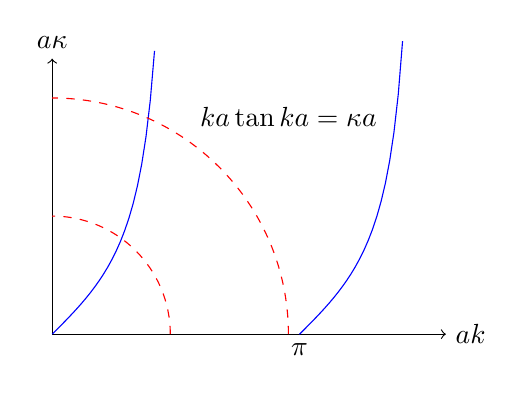
\begin{tikzpicture}[domain=-4:7] [scale=0.8]
\draw[->] (0,0) -- (5,0) node[right] {$ak$};
\draw[->] (0,0) -- (0,3.5) node[above] {$a\kappa$};
\draw[color=blue] plot[domain=0:1.3] (\x,{tan(deg(\x) )});
\draw[color=blue] plot[domain=3.14:4.45] (\x,{tan(deg(\x) )});
\draw [red, dashed] (1.5, 0) arc (0:90:1.5);
\draw [red, dashed] (3, 0) arc (0:90:3);
\draw (3.14,0) node[below]{$\pi$};
\draw (3,3) node[below]{$ka\tan ka=\kappa a$};
\end{tikzpicture}
\hfill
\begin{tikzpicture}[domain=-4:7] [scale=0.8]
\draw[->] (0,0) -- (7.5,0) node[right] {$ak$};
\draw[->] (0,0) -- (0,3.5) node[above] {$a\kappa$};
\draw[color=blue] plot[domain=1.57:2.85] (\x,{-cot(deg(\x) )});
\draw[color=blue] plot[domain=4.7:5.98] (\x,{-cot(deg(\x) )});
\draw [red, dashed] (3, 0) arc (0:90:3);
\draw [red, dashed] (1, 0) arc (0:90:1);
\draw (1.57,0) node[below]{$\pi/2$};
\draw (4.7,0) node[below]{$3\pi/2$};
\draw (4.5,3) node[below]{$-ka\cot ka=\kappa a$};
\end{tikzpicture}
\end{center}
Consider separately the odd solution: similar conditions give $\sin ka=Ae^{-\kappa a}$ and $k\cos ka=-\kappa Ae^{-\kappa a}$, and hence $$-ka\cot(ka)=\kappa a$$ Graphically, we can use 
$$(ka)^2+(\kappa a)^2=\frac{2mV_0}{\hbar^2}a^2$$
(due to conservation of energy) to show there will be no odd bound state, but there will be only one possible even bound state if $$k^2+\kappa^2=\frac{2ma^2V_0}{\hbar^2}<\frac{\pi^2}{4}$$
where $ka=\frac{\pi}{2}$ is the starting point for the odd bound state $-ka\cot(ka)=\kappa a$.\\[5pt]
When this finite square well becomes an infinite square well, the condition $(ka)^2+(\kappa a)^2=\frac{2mV_0}{\hbar^2}a^2$ will intersect the asymptotes of both odd and even bound states, giving us $ka=\frac{\pi}{2}$, $\pi$, $\frac{3\pi}{2}$ and $2\pi$.
\end{ans}
\newpage
\begin{qns}[1D Potential]
A particle is bound in a one-dimensional potential well:
$$V(x)=\infty,\quad x<0;$$
$$V(x)=-V,\quad 0<x<a;$$
$$V(x)=0,\quad x>a$$
in the lowest energy state with total energy $-V/4$.\\[5pt]
Show that the probability that the particle is outside the attractive part of the well is
$$\frac{9\sqrt{3}}{8\pi+12\sqrt{3}}$$
\end{qns}
\begin{ans}
Here, $E=-\frac{V}{4}$. For $0<x<a$, $\frac{d^2\psi}{dx^2}=-\frac{2m}{\hbar^2}(V+E)\psi=-\frac{3mV}{2\hbar^2}\psi:=-k^2\psi$, such that $\psi_I=c_1\sin kx+c_2\cos kx$. For $x>a$, $\frac{d^2\psi}{dx^2}=-\frac{2mE}{\hbar^2}\psi=\frac{mV}{2\hbar^2}\psi:=\kappa^2\psi$, such that $\psi_{II}=c_3e^{\kappa x}+c_4e^{-\kappa x}$. Clearly for $x<0$, $\psi_{III}=0$. The continuity of $\psi$ at $x=0$ gives
$$\psi_I(x=0)=\psi_{III}=0\implies c_2=0$$
The normalizability of this lowest energy state requires $c_3=0$. The continuity of $\psi$ at $x=a$ gives $c_1\sin(ka)=c_4e^{-\kappa a}$ and the continuity of $\frac{d\psi}{dx}$ at $x=a$ gives $kc_1\cos(ka)=-\kappa c_4e^{-\kappa a}$. Note, $\frac{\kappa^2}{k^2}=\frac{1}{3}\implies\kappa=-\frac{1}{\sqrt{3}}k$. Going back to the normalizability condition:
\begin{align}
1&=\int_0^a|\psi_I|^2dx+\int_a^\infty|\psi_{II}|^2dx\nonumber\\&=|c_1|^2\int_0^a\sin^2kxdx+|c_4|^2\int_a^\infty e^{-2\kappa x}dx\nonumber\\&=\frac{|c_1|^2}{2}[a-\frac{1}{2k}\sin 2ka]+\frac{|c_4|^2}{2\kappa}e^{-2\kappa a}:=A+B\nonumber
\end{align}
Then, taking the ratio:
$$\frac{B}{A}=\bigg|\frac{c_4}{c_1}\bigg|^2\frac{e^{-2\kappa a}}{2\kappa}\frac{2}{a-\frac{1}{2k}\sin 2ka}=\frac{9\sqrt{3}}{3\sqrt{3}+8\pi}$$
where $\tan(ka)=-\sqrt{3}\implies ka=-\frac{\pi}{3}+m\pi$, where $m\in\mathbb{Z}^+$ (for it to match continuity, $m=1$) and together with $\kappa=\frac{1}{\sqrt{3}}k$, we have $|\frac{c_4}{c_1}|^2=\frac{3}{4}e^{2\kappa a}$ and $\sin(2ka)=-\frac{\sqrt{3}}{2}$. Then,
$$\frac{1}{B}=1+\frac{A}{B}\implies B=\frac{9\sqrt{3}}{12\sqrt{3}+8\pi}$$
as desired.
\end{ans}
\newpage
\begin{qns}[Harmonic Oscillator]
For a one-dimensional harmonic oscillator oscillating with amplitude $a$, show that the probability of finding the particle in the interval $x$ to $x + dx$ is, according to classical mechanics,
$$P_{cl}(x)dx=\frac{1}{\pi\sqrt{a^2-x^2}}dx,\quad|x|<a;$$
$$P_{cl}(x)dx=0,\quad|x|>a$$
With the aid of sketches compare this probability with the quantum mechanical one for the $n = 1$ eigenstate with normalised eigenfunction
$$\psi_1(x)=\frac{\sqrt{2}}{\pi^{1/4}}\frac{x}{x_0^{3/2}}e^{-x^2/2x_0^2}$$
where $x_0=\sqrt{\hbar/m\omega}$. (Check the normalization of the classical distribution.)
\end{qns}
\begin{ans}
We have $x=A\cos\omega t$ and $v=\frac{dx}{dt}=-\omega a\sin\omega t$, then the classical probability for the particle to be in the range $[x,x+dx]$ is $\frac{2dt}{T}=\frac{2dx}{Tv}=\frac{2dx}{T\omega\sqrt{a^2-x^2}}=\frac{dx}{\pi\sqrt{a^2-x^2}}$, hence
$$\int_{-a}^aP_{cl}dx=\frac{1}{\pi}\int_{-a}^a\frac{1}{\sqrt{a^2-x^2}}dx=\frac{1}{\pi}[\sin^{-1}(1)-\sin^{-1}(-1)]=1$$
as expected. Compare with $P_q(x)dx=|\psi_1|^2dx=\frac{2}{\sqrt{\pi}}\frac{x^2}{x_0^3}e^{-x^2/x_0^2}dx$, which shows two peaks near $x=\pm a$ and $x=\pm a$ are at the points of inflexion of the curve. This is similar to classical one where the probability for the particle to be at $x=\pm a $ is significantly higher.
\end{ans}
\begin{qns}[Harmonic Oscillator]
Find, by inspecting the wavefunctions of a simple harmonic oscillator, the energy eigenvalues of a particle of mass $m$ moving in the potential:
$$V(x)=\infty,\quad x\leq 0;$$
$$V(x)=\frac{1}{2}m\omega^2x^2,\quad x>0$$
\end{qns}
\begin{ans}
The new potential must accommodate $\psi(x=0)=0$ $\forall\psi$. This is only possible if $\psi$ is odd, i.e. $n=2p+1$, where $p\in\mathbb{Z}^+\cup\{0\}$. The energies are $E_n=\hbar\omega((2n+1)+0.5)$ with $n\in\mathbb{Z}^+\cup\{0\}$, instead of $\hbar\omega(n+0.5)$.
\end{ans}
\newpage
\begin{qns}[Correspondence Principle]
Write a few brief notes on the Correspondence Principle, and discuss these with your supervisor.
\end{qns}
\begin{ans}
Correspondence Principle states that in the macroscopic/classical limit where we consider large principle quantum numbers, the results of any quantum problem should match with that of the corresponding classical problem.\\[5pt]
Consider the example of a finite square well. If $E\rightarrow\infty$, the beam of particles will not feel the effects of the potential. Classically, we expect complete transmission. Quantum mechanically, the transmission probability is
$$T=\frac{4k_1^2k_2^2}{4k_1^2k_2^2\cos^2(k_2a)+(k_1^2+k_2^2)\sin^2(k_2a)},\quad\lim_{E\rightarrow\infty}T=1$$
For the example of an infinite square well, in the limit of $n\rightarrow\infty$, we would classically expect a variance of $\sigma_x^2=a^2/12$. This is because the classical probability distribution is uniform, i.e. $f(x)=\frac{1}{a},\quad 0\leq x\leq a$. The variance would be
$$\sigma_x^2=E[X^2]-\mu^2=\int_0^a\frac{x^2}{a}dx-\bigg(\int_0^a\frac{x}{a}\bigg)^2=\frac{a^2}{12}$$
Quantum mechanically, we have the variance in $x$ to be the squared of the uncertainty
$$\sigma_x^2=\langle x^2\rangle-\langle x\rangle^2=\frac{1}{a}\int_0^ax^2\bigg(1-\cos^2\frac{n\pi x}{a}\bigg)dx-\bigg(\int_0^a\frac{2}{a}x\sin^2\frac{n\pi x}{a}dx\bigg)^2=a^2\bigg(\frac{1}{12}-\frac{1}{2n^2\pi^2}\rightarrow\frac{a^2}{12}\bigg)~\text{ as }~n\rightarrow\infty$$
The classical probability distribution for a one-dimensional harmonic oscillator in the interval $|x|<A$ is
$$P_{\text{cl}}=\frac{2dt}{T}=\frac{2dx}{Tv}=\frac{2dx}{T\omega\sqrt{A^2-x^2}}=\frac{dx}{\pi\sqrt{A^2-x^2}}$$
where $x=A\cos\omega t$. For large $n$, the norm of the wavefunction $|\psi_{n\rightarrow\infty}|^2$ will have asymptotic behaviour similar to the classical distribution, where the probability for the particle to be at $x=\pm a$ is significantly higher.\\[5pt]
In the topic of angular momentum, we see that since $[J_i,J_j]\neq 0$ for $i\neq j$, we cannot simultaneously measure the angular momentum in any two directions. But yet, $[J^2,J_i]=0$ $\forall i$, so we can simultaneously measure the total angular momentum and the angular momentum along any direction. In $J$-space, this is represented by a cone where the half-angle of the cone $\theta$ is $\theta=\cos^{-1}\frac{j_z}{j^2}$, where $j_z$ and $j^2$ are the eigenvalues of the operators $J_z$ and $J^2$ on a simultaneous eigenstate. In the limit of large quantum numbers $j\rightarrow\infty$, this angle $\theta\rightarrow 0$. Classically, this is expected since we can definitely simultaneously measure both the angular momentum magnitude and direction.\\[5pt]
Lastly, one recovers the classical dynamical equations of motion when we take the time derivative of the expectation of the corresponding quantum observables. In general, this is obtained from the Ehrenfest's theorem for a generic quantum observable $Q$. 
$$i\hbar\frac{d}{dt}\langle Q\rangle_\psi=\langle [Q,H]\rangle_\Psi+i\hbar\langle\dot{Q}\rangle_\Psi$$
This follows from the definition of expectation and Schr\"{o}dinger's equation. In quantum mechanics, we note that the commutators for a free particle of Hamiltonian $H=\frac{p^2}{2m}+V(x)$ are $[x,H]=\frac{i\hbar}{m}p$ and $[p,H]=-i\hbar V'(x)$.
$$\frac{d}{dt}\langle x\rangle_\Psi=\frac{1}{m}\langle p\rangle_\Psi,\quad\frac{d}{dt}\langle p\rangle_\Psi=-\langle V'(x)\rangle_\Psi$$
which is consistent with the classical counterparts - the Newtonian equations of motion. \\[5pt]
Other examples include
\begin{itemize}
    \item Planck radiation law to converge to Rayleigh-Jeans law when $\hbar\rightarrow 0$
    \item Bohr's model in the limit of $n\rightarrow\infty$ has a spectrum consistent with the classical continuum
    \item Feynman reformulate quantum mechanics (quantum field theory) as extensions of Hamilton's principle of least action (in classical mechanics).
\end{itemize}
See \url{https://physicstoday.scitation.org/doi/pdf/10.1063/1.2916084}
\end{ans}
\newpage
\subsection{Example Sheet 2}
\subsection*{Operator Algebra}
\begin{qns}[Linearity]
Consider the following operations, which act on f(x) as described below, where c is a
constant:
\begin{enumerate}[label=(\alph*)]
    \item $cf(x)$ vertical scaling;
    \item $f(x)+c$ vertical displacement;
    \item $f^2(x)$ squaring;
    \item $\frac{df}{dx}$ differentiation;
    \item $g(x)f(x)$ multiplication by a function;
    \item $f\frac{df}{dx}$;
    \item $\frac{d^2f}{dx^2}$ double differentiation;
    \item $f(cx)$ horizontal scaling;
    \item $\sin(f(x))$;
    \item $f(-x)$ inversion
\end{enumerate}
Which of these operations are linear?\\[5pt]
What are the eigenfunctions of the operations that are linear? (Note: some may not be normalizable.)
\end{qns}
\begin{ans}\leavevmode
\begin{enumerate}[label=(\alph*)]
    \item $c(f_1(x)+f_2(x))=cf_1(x)+cf_2(x)$ linear for any $f(x)$;
    \item $(f_1(x)+c)+(f_2(x)+c)\neq f_1(x)+f_2(x)+c$ not linear;
    \item $(f_1+f_2)^2(x)\neq f_1^2(x)+f_2^2(x)$ not linear;
    \item $\frac{d}{dx}(f_1+f_2)=\frac{df_1}{dx}+\frac{df_2}{dx}$ linear for any exponential function;
    \item $g(x)(f_1(x)+f_2(x))=g(x)f_1(x)+g(x)f_2(x)$ linear for $f(x)=\delta(x-x_0)$;
    \item $(f_1+f_2)\frac{d}{dx}(f_1+f_2)\neq f_1\frac{d}{dx}f_1+f_2\frac{d}{dx}f_2$ not linear;
    \item $\frac{d^2}{dx^2}(f_1+f_2)=\frac{d^2f_1}{dx^2}+\frac{d^2f_2}{dx^2}$ linear for any exponential function;
    \item $f_1(cx)+f_2(cx)=f_1(x)+f_2(x)$ linear for $f(x)$ independent of $x$ or $f(x)=x^b$ for some constant b;
    \item $\sin(f_1(x)+f_2(x))\neq\sin(f_1(x))+\sin(f_2(x))$ not linear;
    \item $f_1(-x)+f_2(-x)=(f_1+f_2)(-x)$ linear only if $f(x)=\pm f(-x)$
\end{enumerate}
\end{ans}
\newpage
\begin{qns}[Hermitian]
Which of the following operators are Hermitian, given that $A$ and $B$ are Hermitian?
$$A+B,\quad cA,\quad AB,\quad AB+BA$$
Show that in one dimension, for functions that tend to zero as $x\rightarrow\pm\infty$, the operator $\frac{d}{dx}$ is not Hermitian, but the operator $-i\hbar\frac{d}{dx}$ is Hermitian. Is the operator $\frac{d^2}{dx^2}$ Hermitian?
\end{qns}
\begin{ans}
Given $A^\dag=A$, $B=B^\dag$, then
$$(A+B)^\dag=A^\dag+B^\dag=A+B$$
$$(cA)^\dag=c^*A^\dag$$
$$(AB)^\dag=B^\dag A^\dag=BA$$
$$(AB+BA)^\dag=B^\dag A^\dag+A^\dag B^\dag =BA+AB$$
The first and fourth is always Hermitian, while the second is Hermitian iff $c=c^*$ and the third is Hermitian iff $[A,B]=0$.\\[5pt]
For $f(x)\rightarrow0$ as $x\rightarrow\pm\infty$, consider
$$\int_{-\infty}^\infty f_2\frac{d}{dx}f_1dx=[f_1f_2]_{-\infty}^\infty -\int_{-\infty}^\infty f_1\frac{df_2}{dx}dx$$
Even if $[f_1f_2]^{\infty}_{-\infty}$ (boundary terms) is zero, $\frac{d}{dx}$ is not Hermitian. But consider
$$\int_{-\infty}^\infty f_2(-i\hbar)\frac{d}{dx}f_1dx=-i\hbar[f_1f_2]_{-\infty}^\infty +i\hbar\int_{-\infty}^\infty f_1\frac{df_2}{dx}dx$$
We can see that if the boundary terms is zero, $-i\hbar\frac{d}{dx}$ is self-adjoint. Finally, consider
$$\int_{-\infty}^\infty f_2\frac{d^2}{dx^2}f_1dx=\bigg[f_2\frac{d}{dx}f_1\bigg]_{-\infty}^\infty -\int_{-\infty}^\infty \frac{df_1}{dx}\frac{df_2}{dx}dx=\bigg[f_2\frac{df_1}{dx}-\frac{df_2}{dx}f_1\bigg]_{-\infty}^\infty+\int_{-\infty}^\infty f_1\frac{d^2f_2}{dx^2}dx$$
If the boundary terms is zero, then $\frac{d^2}{dx^2}$ is Hermitian.
\end{ans}
\begin{qns}[Hermitian]
Show that any non-Hermitian operator $A$ can be written as a linear combination of two Hermitian operators.
\end{qns}
\begin{ans}
We decompose $A$ in the following linear combination:
$$A=\frac{1}{2}(A+A^\dag)+i\frac{1}{2i}(A-A^\dag)$$
the real part (first term) is definitely Hermitian, while the imaginary (second term) is Hermitian when taken together with the imaginary factor $i$.
\end{ans}
\begin{qns}[Orthogonality]
Show that, in one dimension, the state functions $e^{-x^2}$, $xe^{-x^2}$ and $(4x^2-1)e^{-x^2}$ are mutually orthogonal.
\end{qns}
\begin{ans}
$\int_{-\infty}^\infty e^{-x^2}xe^{-x^2}dx$ and $\int_{-\infty}^\infty(4x^2-1)e^{-x^2}xe^{-x^2}dx$ have odd integrands with symmetric limits, and thus evaluate to zero. But
$$\int_{-\infty}^\infty(4x^2-1)e^{-2x^2}dx=4\int_{-\infty}^\infty x^2e^{-2x^2}dx-\int_{-\infty}^\infty e^{-2x^2}dx=\sqrt{\frac{\pi}{2}}\frac{1}{2}-\frac{1}{2}\sqrt{\frac{\pi}{2}}=0$$
So the set $\{e^{-x^2},xe^{-x^2},(4x^2-1)e^{-x^2}\}$ is a mutually orthogonal set with respect to the unit weight function.
\end{ans}
\newpage
\begin{qns}[Orthogonality]
$\phi_1$ and $\phi_2$ are normalised eigenfunctions of observable $A$ which are degenerate, and hence not necessarily orthogonal. If $\langle\phi_1|\phi_2\rangle=c$ and $c$ is real, find linear combinations of $\phi_1$ and $\phi_2$ which are normalised and orthogonal to: (a) $\phi_1$; (b) $\phi_1+\phi_2$.
\end{qns}
\begin{ans}
Given $A\phi_1=\lambda\phi_1$ and $A\phi_2=\lambda\phi_2$ (degenerate) and $\langle\phi_1|\phi_2\rangle=c\in\mathbb{R}$ and not equal to zero (orthogonal). We also have $\langle\phi_1|\phi_1\rangle=\langle\phi_2|\phi_2\rangle=1$ since they are normalized.
\begin{enumerate}[label=(\alph*)]
\item We want to find $c_1$ and $c_2$ such that
$$0=\langle\phi_1|(c_1|\phi_1\rangle+c_2|\phi_2\rangle)=c_1\langle\phi_1|\phi_1\rangle+c_2\langle\phi_1|\phi_2\rangle=c_1+c_2c$$
which give $c_2=-\frac{c_1}{c}$. Upon normalization, we have $\frac{1}{\sqrt{1+c^2}}(|\phi_1\rangle-\frac{1}{c}|\phi_2\rangle)$.
\item We want to find $c_1$ and $c_2$ such that
$$0=(\langle\phi_1|+\langle\phi_2|)(c_1|\phi_1\rangle+c_2|\phi_2\rangle)=c_1\langle\phi_1|\phi_1\rangle+c_2\langle\phi_1|\phi_2\rangle+c_1\langle\phi_2|\phi_1\rangle+c_2\langle\phi_2|\phi_2\rangle=c_1+c_2+(c_1+c_2)c$$
which gives $c_1+c_2=0$ since $1+c$ is not zero. So, upon normalization, we have $\frac{1}{\sqrt{2}}(|\phi_1\rangle-|\phi_2\rangle)$.
\end{enumerate}
\end{ans}
\begin{qns}[Fourier Transform]
A space-domain wavefunction $\psi(x)$ is shifted by $x_0$ to give a new wavefunction $\psi(x-x_0)$. Calculate the corresponding momentum-domain operator. Show that the momentum-domain wavefunction remains normalised even after the operator has been applied.
\end{qns}
\begin{ans}
We will generalize this to three-dimensions. We can Taylor expand $\psi(\mathbf{x}+\mathbf{x_0})$:
$$\psi(\mathbf{x}+\mathbf{x_0})=e^{\mathbf{x_0}\cdot\boldsymbol{\nabla}}\psi(\mathbf{x})$$
but $\mathbf{p}=\frac{\hbar}{i}\boldsymbol{\nabla}$, so $\psi(x-x_0)=e^{-x_0ip/\hbar}\psi(x)$. This is the desired momentum-domain operator, which is merely a global phase which disappears after normalization.
\end{ans}
\begin{qns}[Uncertainty]
Write short notes the following:
\begin{enumerate}[label=(\alph*)]
\item The position of a particle is measured, and it is found to lie within a region having width $\Delta x$. The momentum is then measured, immediately afterwards, and it is found to lie within the range $\Delta p$. If the order of the measurements is changed, so that momentum is measured first and then position, do the results have to be the same?
\item Suppose now that the position of a particle is measured, and it is found to lie within a region having width $\Delta x$, but then its position is measured again. What does quantum mechanics say about the positional uncertainty on the second measurement? If the positional uncertainty is due to the measurement apparatus disturbing the particle, why should the uncertainty be so radically different on the second measurement?
\end{enumerate}
\end{qns}
\begin{ans}
Question is vague. We can assume for (a), the region is a top-hat function. Measuring the dual (momentum-position) quantity gives a sinc distribution. Results will not the same. For (b), inherent positional uncertainty is unchanged since the unknown state (a superposition of known states) has collapsed to one of the known state with definite certainty. In contrast, the uncertainty behind the measurement apparatus is usually assumed to have a Gaussian probabilistic distribution. 
\end{ans}
\newpage
\begin{qns}[Measurement]
Observable $A$ has eigenfunctions $\psi_1$ and  $\psi_2$ with eigenvalues $a_1$ and $a_2$. Observable B has eigenfunctions $\chi_1$ and $\chi_2$ with eigenvalues $b_1$ and $b_2$, which can be expressed as
$$\chi_1=\frac{1}{\sqrt{13}}(2\psi_1+3\psi_2),\quad \chi_2=\frac{1}{\sqrt{13}}(3\psi_1-2\psi_2)$$
$B$ is measured, and value $b_1$ is obtained. What would be the probabilities of getting $a_1$ and $a_2$ in a measurement of A immediately afterwards? After this measurement of $A$, $B$ is again measured; what is the probability of getting $b_1$ again?
\end{qns}
\begin{ans}
Draw a probability tree diagram. Given $b_1$, the probability of getting $a_1$ is $P(a_1|b_1)=|\langle\chi_1|\psi_1\rangle|^2=\frac{4}{13}$ while that of $a_2$ is $P(a_2|
b_1)=|\langle\chi_1|\psi_2\rangle|^2=\frac{9}{13}$. Afterwhich, we act B on the system. Let $P(i|i_1,i_2)$ be the probability of getting $i$ given that we measured $i_1$ first followed by $i_2$ (prior to obtaining $i$), then $$P(b_1|X,b_1)=P(a_1|b_1)P(b_1|a_1,b_1)+P(a_2|b_1)P(b_1|a_2,b_1)=\frac{4}{13}\frac{4}{13}+\frac{9}{13}\frac{9}{13}=\frac{97}{169}$$
\end{ans}
\begin{qns}[Measurement]
For a certain system, the observable $A$ has eigenvalues $\pm1$, with corresponding eigenfunctions $u_+$ and $u_-$ Another observable $B$ also has eigenvalues $\pm1$, but the corresponding eigenfunctions are:
$$v_+=\frac{1}{\sqrt{2}}(u_++u_-),\quad v_-=\frac{1}{\sqrt{2}}(u_+-u_-)$$
Show that $C = A + B$ is an observable and find the possible results of a measurement of $C$.\\[5pt]
Find the probability of obtaining each result when a measurement of $C$ is performed on an atom in the state $u_+$, and (in terms of $u_+$ and $u_-$) the corresponding states $w_\pm$ of the system immediately after the measurement.
\end{qns}
\begin{ans}
Since $A$ and $B$ are observables, by the Postulate of Quantum Mechanics, they may be represented by Hermitian operators. For convenience, I am going to label the operator representation with the name of the observable. The eigenvectors of a Hermitian operator must be mutually orthogonal, i.e. $\langle u_+|u_-\rangle=0$. Without loss of generality, we let $|u_+\rangle=(1,0)$ and $|u_-\rangle=(0,1)$. Then, $|v_\pm\rangle=(1/\sqrt{2})(1,\pm1)$. The matrix representations of $A$ and $B$ can be constructed from the appropriate linear combination of the outer products of their individual eigenvectors, i.e.
$$A=|u_+\rangle\langle u_+|-|u_-\rangle\langle u_-|=\begin{pmatrix}1&0\\0&-1\\\end{pmatrix}$$
$$B=|v_+\rangle\langle v_+|-|v_-\rangle\langle v_-|=\begin{pmatrix}0&1\\1&0\\\end{pmatrix}$$
Since $C=A+B$ is a linear combination of Hermitian operators, $C$ itself will be a Hermitian operator, hence observable. The measurement outcomes of $C$ will be
$$C|u_\pm\rangle=|u_+\rangle\pm|u_-\rangle$$
The eigenvalues of $C$ would be $\pm\sqrt{2}$ and the corresponding eigenvectors are $$|c_\pm\rangle=(\pm\sqrt{2}+1,1)\frac{1}{\sqrt{4\pm2\sqrt{2}}}$$
The corresponding probability for the states $c_\pm$ would be
$$P(|u_+\rangle\rightarrow|c_\pm\rangle)=|\langle u_+|c_\pm\rangle|^2=\bigg|\frac{1\pm\sqrt{2}}{\sqrt{4\pm2\sqrt{2}}}\bigg|^2=\frac{1}{4}(2\pm\sqrt{2})$$
The corresponding state would be 
$$|w_\pm\rangle=\frac{1}{2}\sqrt{2\pm\sqrt{2}}|u_+\rangle\pm\frac{1}{2}\sqrt{2\mp\sqrt{2}}|u_-\rangle$$
\end{ans}
\subsection*{Advanced Operators}
\begin{qns}[Harmonic Oscillator]
By writing $\hat{x}$ and $\hat{p}$ in terms of the raising and lowering operators $\hat{a}^\dag$ and $\hat{a}$, prove that, for the $n$th excited state of a one-dimensional harmonic oscillator, $\sigma_x\sigma_p=(n+0.5)\hbar$.
\end{qns}
\begin{ans}
The one-dimensional harmonic oscillator has the Hamiltonian $\hat{H}=\frac{\hat{p}^2}{2m}+\frac{1}{2}k\hat{x}^2$. We may factorize the Hamiltonian and write $\hat{H}=\hbar\omega(\hat{a}^\dag\hat{a}+0.5)$ where $\hat{a}^\dag=\sqrt{\frac{m\omega}{2\hbar}}(\hat{x}-\frac{i}{m\omega}\hat{p})$ and $\hat{a}=\sqrt{\frac{m\omega}{2\hbar}}(\hat{x}+\frac{i}{m\omega}\hat{p})$. We thus have $\hat{x}=\sqrt{\frac{\hbar}{2m\omega}}(\hat{a}+\hat{a}^\dag)$ and $\hat{p}=i\sqrt{\frac{m\omega\hbar}{2}}(-\hat{a}+\hat{a}^\dag)$. The commutator of the operators is
$$[\hat{a},\hat{a}^\dag]=\frac{1}{2m\hbar\omega}[\hat{p}-im\omega\hat{x},\hat{p}+im\omega\hat{x}]=\frac{1}{2\hbar}2i[\hat{p},\hat{x}]=1$$
The operators $\hat{a}$ and $\hat{a}^\dag$ lower and raise the wavefunction of the $n$th excited state of the harmonic oscillator $\psi_n$ to $\psi_{n-1}$ and $\psi_{n+1}$ respectively. To find the normalization factors, we find
$$||\hat{a}^\dag|\psi_n\rangle||^2=\langle\psi_n|\hat{a}\hat{a}^\dag|\psi_n\rangle=\langle\psi_n|[\hat{a},\hat{a}^\dag]+\hat{a}^\dag\hat{a}|\psi_n\rangle=\langle\psi_n|1+\hat{N}|\psi_n\rangle=n+1$$
$$||\hat{a}|\psi_n\rangle||^2=\langle\psi_n|\hat{a}^\dag\hat{a}|\psi_n\rangle=\langle\psi_n|\hat{N}|\psi_n\rangle=n$$
where $\hat{N}=\hat{a}^\dag\hat{a}$ is the number operator. Hence, $\hat{a}|\psi_n\rangle=\sqrt{n}|\psi_{n-1}\rangle$ and $\hat{a}^\dag|\psi_n\rangle=\sqrt{n+1}|\psi_{n+1}\rangle$. To find the uncertainty, we require $\langle\hat{x}\rangle$, $\langle\hat{x}^2\rangle$ and similarly for $p$. 
$$\langle\psi_n|\hat{x}|\psi_n\rangle=\sqrt{\frac{\hbar}{2m\omega}}\langle\psi_n|\hat{a}+\hat{a}^\dag|\psi_n\rangle=\sqrt{\frac{\hbar}{2m\omega}}(\langle\psi_n|\psi_{n-1}\rangle\sqrt{n}+\langle\psi_n|\psi_{n+1}\rangle\sqrt{n+1})=0$$
$$\langle\psi_n|\hat{p}|\psi_n\rangle=i\sqrt{\frac{m\omega\hbar}{2}}\langle\psi_n|-\hat{a}+\hat{a}^\dag|\psi_n\rangle=i\sqrt{\frac{m\omega\hbar}{2}}(-\langle\psi_n|\psi_{n-1}\rangle\sqrt{n}+\langle\psi_n|\psi_{n+1}\rangle\sqrt{n+1})=0$$
where $\langle\psi_i|\psi_j\rangle=\delta_{ij}$ (the wavefunctions form an orthonormal set).
\begin{align}
\langle\psi_n|\hat{x}^2|\psi_n\rangle&=\frac{\hbar}{2m\omega}\langle\psi_n|(\hat{a}+\hat{a}^\dag)^2|\psi_n\rangle\nonumber\\&=\frac{\hbar}{2m\omega}\langle\psi_n|\hat{a}\hat{a}+\hat{a}\hat{a}^\dag+\hat{a}^\dag\hat{a}+\hat{a}^\dag\hat{a}^\dag|\psi_n\rangle\nonumber\\&=\frac{\hbar}{2m\omega}(n\langle\psi_n|\psi_{n-1}\rangle+(n+1)\langle\psi_n|\psi_{n+1}\rangle)\nonumber
\end{align}
\begin{align}
\langle\psi_n|\hat{p}^2|\psi_n\rangle&=-\frac{m\omega\hbar}{2}\langle\psi_n|(-\hat{a}+\hat{a}^\dag)^2|\psi_n\rangle\nonumber\\&=\frac{m\omega\hbar}{2}\langle\psi_n|\hat{a}\hat{a}-\hat{a}\hat{a}^\dag-\hat{a}^\dag\hat{a}+\hat{a}^\dag\hat{a}^\dag|\psi_n\rangle\nonumber\\&=\frac{m\omega\hbar}{2}(n\langle\psi_n|\psi_{n-1}\rangle+(n+1)\langle\psi_n|\psi_{n+1}\rangle)\nonumber
\end{align}
where $\langle\psi_n|\hat{a}\hat{a}^\dag|\psi_n\rangle=\langle\psi_{n-1}|\sqrt{n}\sqrt{n+1}|\psi_{n+1}\rangle=0$ due to orthonormality. The result is $\langle \hat{x}^2\rangle=\frac{\hbar}{m\omega}(n+0.5)$ and $\langle\hat{p}^2\rangle=m\omega\hbar(n+0.5)$. Hence, 
$$\sigma_x\sigma_{p_x}=\sqrt{\langle\hat{x}^2\rangle\langle\hat{p}^2\rangle}=(n+0.5)\hbar$$
where $\langle\hat{x}\rangle=\langle\hat{p}\rangle=0$.
\end{ans}
\subsection*{Time-dependent quantum mechanics}
\begin{qns}[Ehrenfest]
For a particle of mass $m$ moving freely in one dimension, show that
$$\frac{d\langle \hat{x}^2\rangle}{dt}=\frac{1}{m}\langle\hat{x}\hat{p}+\hat{p}\hat{x}\rangle,\quad\frac{d^2\langle \hat{x}^2\rangle}{dt^2}=\frac{2}{m^2}\langle\hat{p}^2\rangle$$
Show that, if $\frac{d\langle\hat{x}^2\rangle}{dt}=0$ at $t=0$, then at later times $t$:
$$\langle\hat{x}^2\rangle_t=\langle\hat{x}^2\rangle_0+\langle\hat{p}^2\rangle\frac{t^2}{m^2}$$
\end{qns}
\newpage
\begin{ans}
We first prove Ehrenfest Theorem:
$$\frac{d}{dt}\langle\psi|\hat{A}|\psi\rangle=\frac{i}{\hbar}(\langle\psi|\hat{H}\hat{A}|\psi\rangle-\langle\psi|\hat{A}\hat{H}|\psi\rangle)+\langle\frac{\partial\hat{A}}{\partial t}\rangle=\frac{i}{\hbar}\langle[\hat{H},\hat{A}]\rangle+\langle\frac{\partial\hat{A}}{\partial t}\rangle$$
where we used Schrodinger's Equation. We invoke Ehrenfest Theorem for a free particle with Hamiltonian $\hat{H}=\frac{1}{2m}\hat{p}^2$:
$$\frac{d}{dt}\langle\hat{x}^2\rangle=\frac{i}{\hbar}\frac{1}{2m}\langle[\hat{p}^2,\hat{x}^2]\rangle=\frac{i}{2m\hbar}\langle-2\hbar^2-4x\hbar^2\frac{\partial}{\partial x}\rangle=\frac{1}{m}\langle\hat{p}\hat{x}+\hat{x}\hat{p}\rangle$$
where we skipped the details. Invoking Ehrenfest Theorem again,
$$\frac{d^2}{dt^2}\langle\hat{x}^2\rangle=\frac{i}{m\hbar}\bigg(\langle[\hat{H},\hat{p}\hat{x}]\rangle+\langle[\hat{H},\hat{x}\hat{p}]\rangle\bigg)=\frac{2}{m^2}\langle\hat{p}^2\rangle$$
To integrate, we first need to check if $\langle\hat{p}^2\rangle$ is independent of time. To do so, we invoke Ehrenfest Theorem once again.
$$\frac{d}{dt}\langle\hat{p}^2\rangle=\frac{i}{\hbar}\frac{1}{2m}\langle[\hat{p}^2,\hat{p}^2]\rangle=0$$
Then, integrating twice and given $\frac{d}{dt}\langle\hat{x}^2\rangle=0$ and $\langle\hat{x}^2\rangle=\langle\hat{x}^2\rangle_0$ at $t=0$, we obtain our desired relation.
\end{ans}
\begin{qns}[Time Evolution]
For a certain system, $A$ has eigenvalues $a_1$ and $a_2$ corresponding to eigenfunctions:
$$\psi_1=\frac{1}{\sqrt{2}}(u_1+u_2),\quad\psi_2=\frac{1}{\sqrt{2}}(u_1-u_2)$$
where $u_1$ and $u_2$ are stationary states with energies $E_1$ and $E_2$. $A$ is measured and found to have value $a_1$. Find how $\langle A\rangle$ subsequently varies with time.
\end{qns}
\begin{ans}
Writing in bra-ket notation,
$$|\psi_{1,2}(t)\rangle=\frac{1}{\sqrt{2}}\bigg(e^{-iE_1t/\hbar}|u_1\rangle+e^{-iE_2t/\hbar}|u_2\rangle\bigg)$$
Then, the expectation of $\langle\hat{A}\rangle$ (time-dependent function) gives
$$\frac{1}{2}\bigg(\langle u_1|\hat{A}|u_1\rangle+\langle u_2|\hat{A}|u_2\rangle+e^{i\Delta\omega t}\langle u_1|\hat{A}|u_2\rangle+e^{-i\Delta\omega t}\langle u_2|\hat{A}|u_1\rangle\bigg)=\frac{1}{2}\bigg(a_1+a_2+\frac{1}{2}(a_1-a_2)(e^{i\Delta\omega t}+0.5e^{-i\Delta\omega t})\bigg)$$
$$\implies\langle\hat{A}\rangle(t)=\frac{a_1}{2}(1+\cos(\Delta\omega t))+\frac{a_2}{2}(1-\cos(\Delta\omega t))=a_1\cos^2(0.5\Delta\omega t)+a_2\sin^2(0.5\Delta\omega t)$$
where the terms are easily computed by writing $|u_{1,2}\rangle$ in terms of the eigenvectors of $A$, $|\psi_{1,2}\rangle$.
\end{ans}
\begin{qns}
Suppose that $\hat{H}$ is the Hamiltonian of a time-independent system. Using Dirac's bra-ket notation, and bearing in mind the definition of the function of an operator, show that $\hat{H}$ and $\exp[i\hat{H}t]$ commute.
\end{qns}
\begin{ans}
The spectral decomposition of $e^{i\hat{H}t}$ (assuming the matrix power series converges) is $\sum_ke^{iE_kt}|u_k\rangle\langle u_k|$, where $|u_k\rangle$ are the eigenvectors of $\hat{H}$. We thus have
$$[\hat{H},e^{i\hat{H}t}]=\sum_k(E_k|u_k\rangle\langle u_k|u_k\rangle\langle u_k|e^{iE_kt}-e^{iE_kt}|u_k\rangle\langle u_k|u_k\rangle\langle u_k|E_k)=0$$
This is generally true for any convergent function of the operator.
\end{ans}
\begin{qns}
Explain why, when using state vectors, the shift operator introduced in question 6 can be written $\exp[-i\hat{p}x_0/\hbar]$. Show that the operators corresponding to two different shifts $x_{01}$ and $x_{02}$ commute.
\end{qns}
\begin{ans}
We require the translation operator $\hat{T}_{x_0}$ to map $|x\rangle$ to $|x+x_0\rangle$. The properties it must satisfy are (i) unitary; (ii) composition of two translation operators is also a translation operator; (iii) its inverse maps $|x\rangle$ to $|x-x_0\rangle$. Only form of this operator allowed is $\hat{T}_{x_0}=e^{-i\hat{p}x_0/\hbar}$. By the previous problem, $[\hat{T}_{x_0,1},\hat{T}_{x_0,2}]=0$.
\end{ans}
\newpage
\subsection{Example Sheet 3}
\subsection*{Quantum Mechanics in 3D}
\begin{qns}[Angular Momentum Commutation]
Obtain the following commutation relations for the angular momentum operators $\hat{L}=\hat{r}\times\hat{p}$, and comment on the results:
$$[\hat{L}_x,\hat{x}]=0,\quad [\hat{L}_x,\hat{y}]=i\hbar\hat{z}$$
$$[\hat{L}_x,\hat{p}_x]=0,\quad[\hat{L}_x,\hat{p}_y]=i\hbar\hat{p}_z$$
$$[\hat{L}_x,\hat{L^2}]=[\hat{L}_x,\hat{r}^2]=[\hat{L}_x,\hat{p}^2]=0$$
(All other commutation relations follow by the cyclic permutations $x\rightarrow y\rightarrow z\rightarrow x$.)
\end{qns}
\begin{ans}
Using index notation,
\begin{align}
[\hat{L}_i,\hat{r}_l]f&=-i\hbar\epsilon_{jki}\bigg[\hat{r}_j\frac{\partial}{\partial r_k},\hat{r}_l\bigg]f\nonumber\\&=-i\hbar\epsilon_{jki}r_j\frac{\partial r_l}{\partial r_k}f\nonumber\\&=-i\hbar\epsilon_{jki}r_j\delta_{l,k}f\nonumber\\\implies[\hat{L}_i,\hat{r}_k]&=i\hbar\epsilon_{ikj}r_j\nonumber
\end{align}
\begin{align}
[\hat{L}_i,\hat{p}_l]f&=-i\hbar\epsilon_{jki}\frac{\hbar}{i}\bigg[\hat{r}_j\frac{\partial}{\partial r_k},\frac{\partial}{\partial r_l}\bigg]f\nonumber\\&=-\epsilon_{jki}\hbar^2\bigg(r_j\frac{\partial}{\partial r_k}\bigg(\frac{\partial f}{\partial r_l}\bigg)-\frac{\partial}{\partial r_l}\bigg(r_j\frac{\partial f}{\partial r_k}\bigg)\bigg)\nonumber\\&=\hbar^2\epsilon_{jki}\frac{\partial }{\partial r_k}\delta_{j,l}\nonumber\\\implies[\hat{L}_i,\hat{p}_j]&=i\hbar\epsilon_{ijk}\hat{p}_k\nonumber
\end{align}
$$[\hat{L}_i,\hat{L}^2]=[\hat{L}_i,\hat{L}_j\hat{L}_j]=i\hbar\epsilon_{ijk}\hat{L}_k\hat{L}_j+\hat{L}_ji\hbar\epsilon_{ijk}\hat{L}_k=0$$
$$[\hat{L}_i,\hat{r}^2]=[\hat{L}_i,\hat{r}_j\hat{r}_j]=i\hbar\epsilon_{ijk}\hat{r}_k\hat{r}_j+\hat{r}_ji\hbar\epsilon_{ijk}\hat{r}_k=0$$
$$[\hat{L}_i,\hat{p}^2]=[\hat{L}_i,\hat{p}_j\hat{p}_j]=i\hbar\epsilon_{ijk}\hat{p}_k\hat{p}_j+\hat{p}_ji\hbar\epsilon_{ijk}\hat{p}_k=0$$
where the last three results are zero since for instance,  $\epsilon_{ijk}\hat{L}_k\hat{L}_j=-\epsilon_{kji}\hat{L}_k\hat{L}_j=\epsilon_{jki}\hat{L}_j\hat{L}_k$ after relabelling.
\end{ans}
\newpage
\begin{qns}[Angular Momentum Raising and Lowering]
The commutation relations for the angular momentum operators are
$$[\hat{L}_x,\hat{L}_y]=i\hbar\hat{L}_z,\quad [\hat{L}_y,\hat{L}_z]=i\hbar\hat{L}_x,\quad [\hat{L}_z,\hat{L}_x]=i\hbar\hat{L}_y$$
Show that a state cannot be simultaneous eigenfunction of $\hat{L}_x$, $\hat{L}_y$ and $\hat{L}_z$ for non-zero angular momentum $\mathbf{L}$.\\[5pt]
Use the angular momentum raising and lowering operators
$$\hat{L}_\pm=\hat{L}_x\pm i\hat{L}_y=\hbar e^{\pm i\phi}\bigg(\pm\frac{\partial}{\partial\theta}+i\cot\theta\frac{\partial}{\partial\phi}\bigg)$$
to show that
$$\hat{L}^2=\hat{L}_+\hat{L}_-+\hat{L}^2_z-\hbar\hat{L}_z,\quad [\hat{L}_+,\hat{L}_-]=2\hbar\hat{L}_z$$
Hence show that
$$\hat{L}_z=-i\hbar\frac{\partial}{\partial\phi},\quad\hat{L}^2=-\hbar^2\bigg(\frac{1}{\sin\theta}\frac{\partial}{\partial\theta}\sin\theta\frac{\partial}{\partial\theta}+\frac{1}{\sin^2\theta}\frac{\partial^2}{\partial\phi^2}\bigg)$$
Hence obtain the angular momentum quantum numbers for an electron in the Hydrogen atom for the following wavefunctions:
$$\psi(r,\theta,\phi)=R_1(r),\quad\psi(r,\theta,\phi)=R_2(r)\sin\theta e^{i\phi},\quad \psi(r,\theta,\phi)=R_3(r)(3\cos^2\theta-1)$$
\end{qns}
\begin{ans}
If $|\psi\rangle$ is a simultaneous eigenfunction of $\hat{L}_i$ and $\hat{L}_j$ and $\hat{L}_k$, then
$$[\hat{L}_i,\hat{L}_j]|\psi\rangle=l_il_j|\psi\rangle-l_jl_i|\psi\rangle=0$$
but LHS is $i\hbar\epsilon_{ijk}\hat{L}_k|\psi\rangle=0\implies l_k=0$. This contradicts the construction where $l_i$, $l_j$ and $l_k$ were assumed to be not zero in general. Evaluate
$$\hat{L}_\mp\hat{L}_\pm=(\hat{L}_x\mp i\hat{L}_y)(\hat{L}_x\pm i\hat{L}_y)=\hat{L}_x^2+\hat{L}_y^2\pm i[\hat{L}_x,\hat{L}_y]=\hat{L}_x^2+\hat{L}_y^2\mp\hbar\hat{L}_z=\hat{L}^2-\hat{L}_z^2\mp\hbar\hat{L}_z$$
giving us the desired identity. Evaluating the commutator
$$[\hat{L}_+,\hat{L}_-]=-i[\hat{L}_x,\hat{L}_y]+i[\hat{L}_y,\hat{L}_x]=-ii\hbar\hat{L}_z+i(-i\hbar\hat{L}_z)=2\hbar\hat{L}_z$$
Given the suggested transformation (the easier way is by chain rule of partial derivatives),
\begin{eqnarray}
\hat{L}_\pm\hat{L}_\mp&=&\hbar^2e^{\pm i\phi}\bigg(\pm\frac{\partial}{\partial\theta}+i\cot\theta\frac{\partial}{\partial\phi}\bigg)e^{\mp i\phi}\bigg(\mp\frac{\partial}{\partial\theta}+i\cot\theta\frac{\partial}{\partial\phi}\bigg)\nonumber\\&=&\hbar^2e^{\pm i\phi}\frac{\partial}{\partial\theta}e^{\mp i\phi}\bigg(\mp\frac{\partial}{\partial\theta}+i\cot\theta\frac{\partial}{\partial\phi}\bigg)+e^{\pm i\phi}i\cot\theta\frac{\partial}{\partial\phi}e^{\mp i\phi}\bigg(\mp\frac{\partial}{\partial\theta}+i\cot\theta\frac{\partial}{\partial\phi}\bigg)\nonumber\\&=&\hbar^2\bigg(-\frac{\partial^2}{\partial\theta^2}\mp i\frac{\partial}{\partial\phi}-\cot\theta\frac{\partial}{\partial\theta}-\cot^2\theta\frac{\partial^2}{\partial\phi^2}\bigg)
\nonumber
\end{eqnarray}
But $[\hat{L}_+,\hat{L}_-]=2\hbar\hat{L}_z\implies\hat{L}_z=-i\hbar\frac{\partial}{\partial\phi}$. Hence, $\hat{L}^2$ will be
$$\hat{L}^2=\hbar^2\bigg(-\frac{\partial^2}{\partial\theta^2}- i\frac{\partial}{\partial\phi}-\cot\theta\frac{\partial}{\partial\theta}-\cot^2\theta\frac{\partial^2}{\partial\phi^2}\bigg)-\hbar^2\frac{\partial^2}{\partial\phi^2}+i\hbar^2\frac{\partial}{\partial\phi}=-\hbar^2\bigg(\frac{1}{\sin\theta}\frac{\partial}{\partial\theta}\sin\theta\frac{\partial}{\partial\theta}+\frac{1}{\sin^2\theta}\frac{\partial^2}{\partial\phi^2}\bigg)$$
For the various wavefunctions, we have
$$\hat{L}^2R_1(r)=0,\quad\hat{L}_zR_1(r)=0\implies \ell=0,~m_\ell=0$$
$$\hat{L}^2R_2(r)\sin\theta e^{i\phi}=-R_2(r)\hbar^2e^{i\phi}\frac{1}{\sin\theta}\frac{d}{d\theta}\bigg(\sin\theta\frac{d}{d\theta}\sin\theta\bigg)-R_2(r)\hbar^2\bigg(\frac{1}{\sin^2\theta}\bigg)\frac{\partial^2}{\partial\phi^2}e^{i\phi}\sin\theta=\hbar^2R_2(r)e^{i\phi}\sin\theta\implies\ell=1$$
$$\hat{L}_zR_2(r)\sin\theta e^{i\phi}=i\hbar R_2(r)\sin\theta\bigg(-\frac{\partial}{\partial\phi}e^{i\phi}\bigg)=\hbar R_2(r)\sin\theta e^{i\phi}\implies m_\ell=1$$
$$\hat{L}^2R_3(r)(3\cos^2\theta-1)=6\hbar^2R_3(r)(-1+3\cos^2\theta),\quad\hat{L}_zR_3(r)(3\cos^2\theta-1)=0\implies \ell=2,~m_\ell=0$$
\end{ans}

\begin{qns}[Angular Momentum Commutation]
The orthogonal wavefunctions $\psi_x=xf(r)$, $\psi_y=yf(r)$ and  $\psi_z=zf(r)$ represent three of the electronic bound state solutions for a hydrogen atom. Prove the relations shown in
the first row of the table below:
$$\hat{L}_x\psi_x=0,\quad\hat{L}_x\psi_y=i\hbar\psi_z,\quad\hat{L}_x\psi_z=-i\hbar\psi_y$$
$$\hat{L}_y\psi_x=-i\hbar\psi_z,\quad\hat{L}_y\psi_y=0,\quad\hat{L}_y\psi_z=i\hbar\psi_x$$
$$\hat{L}_z\psi_x=i\hbar\psi_y,\quad\hat{L}_z\psi_y=-i\hbar\psi_x,\quad\hat{L}_z\psi_z=0$$
Use the results in the table to prove that the expectation value of each component of the angular momentum of any one of $\psi_x$, $\psi_y$ and $\psi_z$ is zero. Show, however, that each is an eigenfunction of the operator $\hat{L}^2=\hat{L}_x^2+\hat{L}_y^2+\hat{L}_z^2$ and determine the eigenvalue.\\[5pt]
Show that the linear combinations $\psi_\pm=\psi_x\pm i\psi_y$ are eigenfunctions of $\hat{L}_z$ and determine their orbital angular momentum quantum numbers $m$ and $\ell$.
\end{qns}
\begin{ans}
We use index notation and define $\psi_q$ to be $x_qf(\sqrt{x_rx_r})$.
$$\hat{L}_p\psi_q=-i\hbar\epsilon_{jkp}x_j\frac{\partial}{\partial x_k}x_qf(\sqrt{x_rx_r})=-i\hbar\epsilon_{jkp}x_j\delta_{qk}f(\sqrt{x_rx_r})-i\hbar\epsilon_{jkp}x_jx_q\frac{x_k}{x_rx_r}f'(\sqrt{x_rx_r})$$
but $x_jx_k$ is a symmetric tensor and upon contracting with an anti-symmetric pseudo-tensor $\epsilon_{ijk}$, the result is zero. Hence, $\hat{L}_p\psi_q=i\hbar\epsilon_{pqj}x_jf(\sqrt{x_rx_r})$. The expectation will be
$$\langle\psi_q|\hat{L}_p|\psi_q\rangle=\langle\psi_q|\psi_j\rangle i\hbar\epsilon_{pqj}=0$$
where $|\psi_j\rangle\neq0$ if $q\neq j$, and given that distinct states are orthogonal.
$$\hat{L}^2|\psi_q\rangle=\hat{L}_p\hat{L}_p|\psi_q\rangle=\hat{L}_pi\hbar\epsilon_{pqj}|\psi_j\rangle=-\hbar^2\epsilon_{pjr}\epsilon_{pqj}|\psi_r\rangle=2\hbar^2\delta_{rq}|\psi_r\rangle=2\hbar^2|\psi_q\rangle$$
Each state is an eigenvector of $\hat{L}^2$ with eigenvalue $2\hbar^2$.
$$\hat{L}_z|\psi_\pm\rangle=\hat{L}_z|\psi_x\rangle\pm i\hat{L}_z|\psi_y\rangle=i\hbar|\psi_y\rangle\pm\hbar|\psi_x\rangle=\pm\hbar|\psi_\pm\rangle$$
$|\psi_\pm\rangle$ is an eigenvector of $\hat{L}_z$ with eigenvalue $m_\ell=\pm 1$. Moreover,
$$\hat{L}^2|\psi_\pm\rangle=\hat{L}^2|\psi_x\rangle\pm i\hat{L}^2|\psi_y\rangle=2\hbar^2|\psi_\pm\rangle$$
$|\psi_\pm\rangle$ is an eigenvector of $\hat{L}^2$ with eigenvalue $2\hbar^2\implies \ell(\ell+1)=2\implies\ell=1$.
\end{ans}
\newpage
\textcolor{darkblue}{For Questions 4 and 5 you can use the following information about a Hydrogen atom.\\[5pt]
The normalised wavefunctions $Y_{\ell m_\ell}(\theta,\phi)$ for $\ell=0,1$ and 2 are:
$$Y_{00}=\sqrt{\frac{1}{4\pi}}$$
$$Y_{10}=\sqrt{\frac{3}{4\pi}}\cos\theta,\quad Y_{1\pm1}=\mp\sqrt{\frac{3}{8\pi}}\sin\theta e^{\pm i\phi}$$
$$Y_{20}=\sqrt{\frac{5}{16\pi}}(3\cos^2\theta-1),\quad Y_{2\pm1}=\mp\sqrt{\frac{15}{8\pi}}\sin\theta\cos\theta e^{\pm i\phi},\quad Y_{2\pm2}=\sqrt{\frac{15}{32\pi}}\sin^2\theta e^{\pm 2i\phi}$$
and the normalised hydrogen-like radial wavefunctions $R_{n\ell}$ for $n = 1, 2$ are:
$$R_{10}=(Z/a_0)^{3/2}2e^{-Zr/a_0}$$
$$R_{20}=(Z/2a_0)^{3/2}(2-Zr/a_0)e^{-Zr/2a_0}$$
$$R_{21}=(Z/2a_0)^{3/2}(1/\sqrt{3})(Zr/a_0)e^{-Zr/2a_0}$$
where $a_0$ is the Bohr radius.\\[5pt]
Note also that $\int_0^\infty x^ne^{-x}dx=n!$.}
\begin{qns}[Hydrogen Atom]
Confirm, for the cases $\ell= 1$ and $\ell=2$, that
$$\sum_{m_\ell=-\ell}^{m_\ell=\ell}|Y_{\ell m_\ell}|^2=\text{ constant}$$
Discuss the significance of this result for the electron probability distributions in the hydrogen atom. (The theorem for general $\ell$ follows from an addition formula for Legendre polynomials, see Whittaker and Watson, p. 327.)
\end{qns}
\begin{ans}
For $\ell=1$ and $\ell=2$ respectively, 
$$\sum_{m_\ell=-1}^1|Y_{\ell,m_\ell}|^2=|Y_{1,-1}|^2+|Y_{1,0}|^2+|Y_{1,1}|^2=\frac{2}{8\pi}\sin^2\theta+\frac{3}{8\pi}\sin^2\theta+\frac{3}{4\pi}\cos^2\theta=\frac{3}{4\pi}$$
\begin{eqnarray}
\sum_{m_\ell=-2}^2|Y_{\ell,m_\ell}|^2&=&|Y_{2,-2}|^2+|Y_{2,-1}|^2+|Y_{2,0}|^2+|Y_{2,1}|^2+|Y_{2,2}|^2\nonumber\\&=&\frac{15\times 2}{32\pi}\sin^4\theta+\frac{15\times 2}{8\pi}\sin^2\theta\cos^2\theta+\frac{5}{16\pi}(3\cos^2\theta-1)^2\nonumber\\&=&\frac{15}{16\pi}\sin^4\theta+\frac{15}{4\pi}\cos^2\theta(1-\cos^2\theta)+\frac{5}{16\pi}(9\cos^4\theta-6\cos^2\theta+1)\nonumber\\&=&\frac{15}{16\pi}((\sin^2\theta)^2-(\cos^2\theta)^2)+\frac{30}{16\pi}\cos^2\theta+\frac{5}{16\pi}\nonumber\\&=&\frac{5}{4\pi}\nonumber
\end{eqnarray}
In another words, $\sum_{m_\ell=-l}^l|Y_{\ell,m_\ell}|^2=\frac{2\ell+1}{4\pi}$, where there are $2\ell+1$ number of $m_\ell$ values. $|Y_{\ell,m_\ell}|^2$ is independent of $\theta$ and $\phi$ and so the electron probability distribution has no angular dependence. There is equal superposition for filled shells.
\end{ans}
\newpage
\begin{qns}[Hydrogen Atom]
An electron is in the ground state of a hydrogen-like atom with nuclear charge $+Ze$.
\begin{enumerate}[label=(\alph*)]
\item What is its average distance from the nucleus?
\item At what distance from the nucleus is it most likely to be found?
\item Show that the expectation value of the potential energy operator of the electron is $-\frac{Z^2e^2}{4\pi\epsilon_0a_0}$.
\item Show that the expectation value of the kinetic energy operator is $\frac{Z^2e^2}{8\pi\epsilon_0a_0}$.
\item Hence verify that the expectation value of the Hamiltonian is the energy of the ground state. 
\end{enumerate}
\end{qns}
\begin{ans}
The ground state wavefunction of the Hydrogen-like atom is $\psi=Y_{00}R_{10}=\frac{1}{\sqrt{4\pi}}(Z/a_0)^{3/2}2e^{-Zr/a_0}$. Also, we will invoke the identity $\int_0^\infty r^ne^{-\alpha r}dr=\frac{n!}{\alpha^{n+1}}$.
\begin{enumerate}[label=(\alph*)]
\item The average distance is
$$\langle r\rangle=\int_{\mathbb{R}^3}\psi^*r\psi dV=\frac{Z^3}{\pi a_0^3}\int_0^\pi\sin\theta d\theta\int_0^{2\pi}d\phi\int_0^\infty r^3e^{-2Zr/a_0}dr=\frac{4\pi Z^3}{\pi a_0^3}\frac{6}{(2Z/a_0)^4}=\frac{3a_0}{2Z}$$
\item The probability of finding the particle in a region $[r,r+dr]$ is
$$P(r)dr=\frac{4}{4\pi}\frac{Z^3}{a_0^3}e^{-2Zr/a_0}r^2\int_0^{2\pi}\int_0^\pi\sin\theta d\theta d\phi dr=\frac{4Z^3}{a_0^3}e^{-2Zr/a_0}r^2dr$$
To find the radius at which the probability distribution is maximum,
$$0=\frac{dP(r)}{dr}\implies 0=2re^{-2Zr/a_0}-\frac{2Z}{a_0}r^2e^{-2Zr/a_0}\implies r=\frac{a_0}{Z}$$
\item The expectation for the potential energy is
$$\langle V\rangle=-\frac{Ze^2}{4\pi\epsilon_0}\frac{4Z^3}{a_0^3}\int_0^\infty re^{-2Zr/a_0}dr=\frac{-Z^4e^2}{\pi\epsilon_0a^3}\frac{a_0^2}{4Z^2}=-\frac{Z^2e^2}{4\pi\epsilon_0a_0}$$
\item The expectation for the kinetic energy is
\begin{eqnarray}
\langle K\rangle&=&-\frac{\hbar^2}{2m}\int_0^\infty\frac{4}{4\pi}\frac{Z^3}{a_0^3}r^2e^{-Zr/a_0}\frac{1}{r^2}\frac{\partial}{\partial r}\bigg(r^2\frac{\partial}{\partial r}e^{-Zr/a_0}\bigg)dr\int_0^\pi\sin\theta d\theta\int_0^{2\pi}d\phi\nonumber\\&=&\frac{4Z^4\hbar^2}{2ma_0^4}\int_0^\infty e^{-Zr/a_0}\frac{\partial}{\partial r}(r^2e^{-Zr/a_0})dr\nonumber\\&=&\frac{4\hbar^2Z^4}{ma_0^4}\int_0^\infty re^{-2Zr/a_0}dr-\frac{2\hbar^2Z^5}{ma_0^5}\int_0^\infty r^2e^{-2Zr/a_0}dr\nonumber\\&=&\frac{4\hbar^2Z^4}{ma_0^4}\frac{a_0^2}{4Z^2}-\frac{2\hbar^2Z^5}{ma_0^5}\frac{a_0^3}{4Z^3}\nonumber\\&=&\frac{Z^2e^2}{8\pi\epsilon_0a_0}\nonumber
\end{eqnarray}
where $a_0=\frac{4\pi\epsilon_0\hbar^2}{me^2}$ by definition.
\item The expectation for the Hamiltonian is the sum of that of the kinetic energy and potential energy, which gives $-\frac{Z^2e^2}{8\pi\epsilon_0a_0}$.
\end{enumerate}
\end{ans}
\newpage
\begin{qns}[3D Isotropic Harmonic Oscillator]
The potential energy for a three-dimensional harmonic oscillator of mass m and frequency $\omega$ is $V(x,y,z)=\frac{1}{2}m\omega^2(x^2+y^2+z^2)$.\\[5pt]
What are the energies and degeneracies of the three lowest levels?\\[5pt]
Show that the degeneracy of the $n$th excited level is $\frac{1}{2}(n+1)(n+2)$.
\end{qns}
\begin{ans}
The Hamiltonian of the 3D Isotropic Harmonic Oscillator is separable, and is equivalent to the product of three 1D Harmonic Oscillator. The energy is thus 
$$E=(n_x+0.5)\hbar\omega+(n_y+0.5)\hbar\omega+(n_z+0.5)\hbar\omega$$
When $n_x=n_y=n_z=0$, $E=\frac{3}{2}\hbar\omega$ and there is only one possible level. When $n_x=1$, $n_y=n_z=0$ (or two other permutations), $E=\frac{5}{2}\hbar\omega$ and the degeneracy is 3. When $n_x=1$, $n_y=1$, $n_z=0$ (or two other permutations), or equivalently, $n_x=2$, $n_y=0$, $n_z=0$ (or two other permutations), $E=\frac{7}{2}\hbar\omega$ and the degeneracy is 6.\\[5pt]
Consider $n$ quanta, to be filled into $N$ boxes. There are $N-1$ number of partitions. So the number of ways to arrange them is $\frac{(N-1+n)!}{(N-1)!n!}$ since there are $N-1$ number of identical partitions and $n$ number of identical quanta. For $N=3$, we have $\frac{(n+2)!}{2!n!}=\frac{1}{2}(n+1)(n+2)$. 
\end{ans}
\subsection*{Two particle systems}
\begin{qns}[Two Body Problem]
In a one-dimensional system two particles each of mass $m$ interact through the potential $\frac{1}{2}m\omega^2(x_1-x_2)^2$ where $x_1$ and $x_2$ are their position coordinates. Find the energy levels of the system when its centre of mass is at rest.
\end{qns}
\begin{ans}
We transform coordinates, i.e.
$$\hat{P}=\hat{p}_1+\hat{p_2},\quad \hat{p}=\frac{1}{2}(\hat{p_1}-\hat{p}_2)$$
$$\hat{X}=\frac{1}{2}(\hat{x}_1+\hat{x}_2),\quad\hat{x}=\hat{x}_1-\hat{x}_2$$
The Hamiltonian becomes
$$\hat{H}=\frac{\hat{P}^2}{2m}+\frac{\hat{p}^2}{2(m/2)}+\frac{1}{2}m\omega^2\hat{x}^2$$
Given $\hat{P}=0$, we have
$$\hat{H}=\frac{(\sqrt{2}p)^2}{2m}+\frac{1}{2}2m(\omega/\sqrt{2})^2x^2$$
This has the form of a harmonic oscillator with energy to be $E=(n+0.5)\hbar\omega\sqrt{2}$.
\end{ans}
\begin{qns}[Two Body Problem]
The Hamiltonian $\hat{H}$ of two interacting particles a and b is given by
$$\hat{H}=\frac{\hat{p}_a^2}{2m_a}+\frac{\hat{p}_b^2}{2m_b}+\hat{V}(|\mathbf{r}|)$$
where $\mathbf{r}=\mathbf{r_a}-\mathbf{r_b}$ is the relative position of the particles. \\[5pt]
Derive the commutation relations of the centre-of-mass and relative position and momentum operators $\hat{R}$, $\hat{r}$, $\hat{P}$ and $\hat{p}$, where:
$$\hat{\mathbf{R}}=\frac{m_a\hat{\mathbf{r}}_a+m_b\hat{\mathbf{r}}_b}{m_a+m_b};\hat{\mathbf{p}}=\frac{m_am_b}{m_a+m_b}\bigg(\frac{\hat{\mathbf{p}}_a}{m_a}-\frac{\hat{\mathbf{p}}_b}{m_b}\bigg)$$
Comment on your results.
\end{qns}
\begin{ans}
The commutators are $[\hat{P},\hat{p}]=0$, $[\hat{R},\hat{r}]=0$, $[\hat{r}_j,\hat{P}_k]=0$, $[\hat{R}_j,\hat{p}_k]=0$ and $[\hat{R}_j,\hat{P}_k]=i\hbar\delta_{jk}$ and $[\hat{r}_j,\hat{p}_k]=i\hbar\delta_{jk}$. Note that $\hat{V}(|\mathbf{r}|)$ is an internal potential.\\[5pt]
The classical description of decoupling a two-body problem still holds for the quantum cases. In another words, the position of centre of mass and relative momentum are compatible observables.
\end{ans}
\newpage
\subsection{Example Sheet 4}
\subsection*{Spin and matrix mechanics}
\begin{qns}[Angular momentum ladder operators]
Denote the eigenfunctions of $\hat{L}^2$ and $\hat{L}_z$ with eigenvalues $\ell= 1$ and $m_\ell =-1$, 0, 1 by $|\phi_{-1}\rangle$, $|\phi_0\rangle$, $|\phi_1\rangle$. Use the ladder operators $\hat{L}_+$ and $\hat{L}_-$ to find the eigenfunctions of $\hat{L}_x$ in terms of those of $\hat{L}_z$.\\[5pt]
A beam of atoms with zero spin and in the state $\ell= 1$ is traveling along the $y$-axis and passes through an x-Stern-Gerlach apparatus. The emerging beam with $m_\ell = 1$ is passed through a z-Stern-Gerlach apparatus. Into how many beams is this beam further split and what are the relative numbers of atoms in them?\\[5pt]
What happens if the other two beams from the first Stern-Gerlach apparatus are treated in the same way?
\end{qns}
\begin{ans}
We have the simultaneous eigenstates to satisfy
$$\hat{L}^2|\phi_i\rangle=\hbar^2 1(1+1)|\phi_i\rangle=2\hbar^2|\phi_i\rangle,\quad\hat{L}_z|\phi_i\rangle=\hbar i|\phi_\rangle,\quad i=0,\pm1$$
For now, temporarily denote $|\phi_i\rangle$ as $|\ell=1,m_\ell=i\rangle$, then the ladder operators must act like
$$\hat{L}_\pm|1,i\rangle=C_{\pm}|1,i\pm1\rangle$$
where the coefficients are the norm of the resultant state.
\begin{align}
    C_\pm&=\langle 1,i|(\hat{L}_x\mp i\hat{L}_y)(\hat{L}_x\pm i\hat{L}_y)|1,i\rangle\nonumber\\&=\langle 1,i|\hat{L}_x^2+\hat{L}_y^2\pm i[\hat{L}_x,\hat{L}_y]|1,i\rangle\nonumber\\&=\langle 1,i|\hat{L}^2-\hat{L}_z^2\pm i(i\hbar)\hat{L}_z|1,i\rangle\nonumber\\&=\hbar^2(\ell(\ell+1)-m^2\mp m)\nonumber
\end{align}
Hence, the resultant image of the simultaneous eigenstates will be
$$\hat{L}_+|\phi_{-1}\rangle=\sqrt{2}\hbar|\phi_0\rangle,~\hat{L}_-|\phi_{-1}\rangle=0,\quad\hat{L}_\pm|\phi_0\rangle=\hbar\sqrt{2}|\phi_{\pm 1}\rangle,\quad\hat{L}_-|\phi_{+1}\rangle=\hbar\sqrt{2}|\phi_0\rangle,~\hat{L}_+|\phi_{+1}\rangle=0$$
But $\hat{L}_x=0.5(\hat{L}_++\hat{L}_-)$, so $\hat{L}_x|\phi_\pm1\rangle=(\hbar/\sqrt{2})|\phi_0\rangle$. Also, $\hat{L}_x|\phi_0\rangle=(\hbar/\sqrt{2})(|\phi_{+1}\rangle+|\phi_{-1}\rangle)$. We wish to find the eigenfunctions of $\hat{L}_x$. Let this be
$$|\Phi\rangle=c_1|\phi_1\rangle+c_{-1}|\phi_{-1}\rangle+c_0|\phi_0\rangle\implies\hat{L}_x|\phi\rangle=(c_1+c_{-1})\frac{\hbar}{\sqrt{2}}|\phi_0\rangle+c_0\frac{\hbar}{\sqrt{2}}(|\phi_1\rangle+|\phi_{-1}\rangle)$$
Observe that $c_0=0$ could give a solution $c_1=-c_{-1}$. This eigenvector must be normalized, so we have $|\Phi\rangle=\frac{1}{\sqrt{2}}(|\phi_1\rangle-|\phi_{-1}\rangle)$ with corresponding eigenvalue 0, i.e. $\hat{L}_x|\Phi\rangle=0\hbar|\Phi\rangle$. Another solution by inspection is $c_1=c_{-1}=1$ that admits $c_0=\pm\sqrt{2}$. Normalizing gives $|\Phi\rangle=\frac{1}{2}(|\phi_1\rangle+|\phi_{-1}\rangle\pm\sqrt{2}|\phi_0\rangle)$. The corresponding eigenvalue is $\pm\hbar$, i.e. $\hat{L}_x|\Phi\rangle=\pm\hbar|\Phi\rangle$. Equivalently, the above procedure diagonalizes the following matrix in terms of the eigenbasis of $\hat{L}_z$  $\{|\phi_1\rangle,|\phi_{-1}\rangle,|\phi_0\rangle\}$:
$$\hat{L}_x=\frac{\hbar}{\sqrt{2}}\begin{pmatrix}0&1&0\\1&0&1\\0&1&0\\\end{pmatrix}$$
The action of the first Stern-Gerlach apparatus does not concern us. The emerging beam with $m_\ell$ value obtained after applying $\hat{L}_x$ on the initial state. So, the state corresponding to $m_\ell=\pm1$ will be $\frac{1}{2}(|\phi_1\rangle+|\phi_{-1}\rangle\pm\sqrt{2}|\phi_0\rangle)$. Pass this state through $\hat{L}_z$ and the measurement outcome will be a triplet signal:
\begin{itemize}
    \item $|\phi_\pm1\rangle$ with eigenvalue $\pm\hbar$ and probability $(1/2)^2=1/4$,
    \item $|\phi_0\rangle$ with eigenvalue 0 and probability $(1/\sqrt{2})^2=1/2$.
\end{itemize}
The relative number of atoms would be 1:2:1. For the $m_\ell=0$ state, this is $\frac{1}{\sqrt{2}}(|\phi_1\rangle-|\phi_{-1}\rangle$ and will give a doublet signal. The eigenvalue corresponding to $|\phi_\pm1\rangle$ each will be $+1$ with probability 1/2.
\end{ans}
\newpage
\begin{qns}[Addition of angular momentum]
Derive the eigenfunctions of the operators $\hat{J}^2$ and $\hat{J}_z$ in terms of the eigenfunctions of $\hat{L}^2$, $\hat{S}^2$, $\hat{L}_z$ and $\hat{S}_z$  for the case $\ell= 1$, $s = \frac{1}{2}$.
\end{qns}
\begin{ans}
The composite Hilbert space will be $\mathcal{H}_L\otimes\mathcal{H}_S$ and the total angular momentum is
$$\hat{J}=\hat{L}\otimes\Id+\Id\otimes \hat{S}$$
acting on the generic state $|\Psi\rangle=|\ell,m_\ell\rangle\otimes|s,m_s\rangle$. Then we define the operators
$$\hat{J}^2=\hat{L}^2\otimes\Id+\Id\otimes \hat{S}^2+2\hat{L}\otimes \hat{S}$$
$$\hat{J}_z=\hat{L}_z\otimes\Id+\Id\otimes \hat{S}_z$$
The action of $\hat{J}^2$ and $\hat{J}_z$ on $|\Psi\rangle=|\ell,m_\ell\rangle\otimes|s,m_s\rangle$ is
$$\hat{J}_z|\ell,m_\ell\rangle\otimes|s,m_s\rangle=(\hat{L}_{z}\otimes\Id+\Id\otimes \hat{S}_{z})|\ell,m_\ell\rangle\otimes|s,m_s\rangle=\hbar(\ell+s)|\ell,m_\ell\rangle\otimes|s,m_s\rangle$$
$$\hat{J}^2|\ell,m_\ell\rangle\otimes|s,m_s\rangle=[\ell(\ell+1)+s(s+1)+2\ell s]\hbar^2|\ell,m_\ell\rangle\otimes|s,m_s\rangle=(\ell+s)(\ell+s+1)\hbar^2|\ell,m_\ell\rangle\otimes|s,m_s\rangle$$
The results suggest we could have denoted our generic state $|\Psi\rangle$ as $|j,m_j\rangle$ where 
$$|\ell-s|\leq j\leq\ell+s,\quad -j\leq m_j\leq j$$
We define the lowering operator to be
$$\hat{J}_-=\hat{L}_-\otimes\Id+\Id\otimes \hat{S}_-$$
Consider its action on the highest weight state $|j,m_j=j\rangle$:
$$\hat{J}_-|j,j\rangle=\hbar\sqrt{2j}|j,j-1\rangle$$
but this should be equal to
$$(\hat{L}_-\otimes\Id+\Id\otimes \hat{S}_-)|\ell,\ell\rangle\otimes|s,s\rangle=\hbar\sqrt{2\ell}|\ell,\ell-1\rangle\otimes|s,s\rangle+\hbar\sqrt{2s}|\ell,\ell\rangle|s,s-1\rangle$$
Hence, the lowered state will be
\begin{equation}
|j,j-1\rangle=\sqrt{\ell/j}|\ell,\ell-1\rangle\otimes|s,s\rangle+\sqrt{s/j}|\ell,\ell\rangle\otimes|s,s-1\rangle\tag{*}
\end{equation}
The state $|j-1,j-1\rangle$ must be orthogonal to $|j,j-1\rangle$, so
\begin{equation}
|j-1,j-1\rangle=\sqrt{s/j}|\ell,\ell-1\rangle\otimes|s,s\rangle-\sqrt{\ell/j}|\ell,\ell\rangle\otimes|s,s-1\rangle\tag{\dag}
\end{equation}
Here, we consider $\ell=1$ and $s=0.5$. Apply this procedure to our highest weight state $|1.5,1.5\rangle=|1,1\rangle|0.5,0.5\rangle$. (*) gives
$$|1.5,0.5\rangle=\sqrt{2/3}|1,0\rangle|0.5,0.5\rangle+\frac{1}{\sqrt{3}}|1,1\rangle|0.5,-0.5\rangle$$
For $j=1.5$, $m_j=-1/2$, we must have $\ell=1,0.5$ and this restricts $m_\ell$ to be $-1,0.5$. Hence,
$$|1.5,-0.5\rangle=|1,-1\rangle|0.5,0.5\rangle$$
For $j=1.5$, $m_j=-1.5$, we must have $\ell=1,0.5$ again and this restricts $m_\ell$ to be $-1,-0.5$. Hence,
$$|1.5,-1.5\rangle=|1,-1\rangle|0.5,-0.5\rangle$$
From ($\dag$) and (*) respectively,
$$|0.5,0.5\rangle=(1/\sqrt{3})|1,0\rangle|0.5,0.5\rangle-\sqrt{2/3}|1,1\rangle|0.5,-0.5\rangle$$
$$|0.5,-0.5\rangle=\sqrt{2/3}|1,-1\rangle|0.5,0.5\rangle-(1/\sqrt{3})|1,0\rangle|0.5,-0.5\rangle$$
Altogether this are $4+2=3\times 2$ states. 4 states for $j=1.5$ and 2 for $j=0.5$; 3 states for spin 1 and 2 states from spin 0.5. We denote this result as $1\otimes0.5=1.5\oplus0.5$, where the resultant vector spaces on both sides have the same dimensions.
\end{ans}
\newpage
\begin{qns}[Singlet and triplet]
For a system involving two particles of spin $s_1=\frac{1}{2}$ and $s_2=\frac{1}{2}$, find the eigenvalues of $\hat{s}_1\cdot\hat{s}_2$ for the `anti-parallel' spin singlet state and the `parallel' spin triplet states, and comment on your results.
\end{qns}
\begin{ans}
Similar to the previous question but the operator is now defined as
$$\hat{s}=\hat{s}_1\otimes\Id+\Id\otimes s_2$$
The same result applies
\begin{equation}
|s,s-1\rangle=\sqrt{s_1/s}|s_1,s_1-1\rangle\otimes|s_2,s_2\rangle+\sqrt{s_2/s}|s_1,s_1\rangle\otimes|s_2,s_2-1\rangle\tag{*}
\end{equation}
\begin{equation}
|s-1,s-1\rangle=\sqrt{s_2/s}|s_1,s_1-1\rangle\otimes|s_2,s_2\rangle-\sqrt{s_1/s}|s_1,s_1\rangle\otimes|s_2,s_2-1\rangle\tag{\dag}
\end{equation}
Now $s_1=s_2=0.5$, we have the highest weight state ($s=s_1+s_2,m_s=s$) to be $$|1,1\rangle=|0.5,0.5\rangle|0.5,0.5\rangle:=|\uparrow\rangle|\uparrow\rangle$$ 
Here, LHS is $|s,m_s\rangle$ while RHS is $|s_1,m_{s,1}\rangle|s_2m_{s,2}\rangle$. Apply (*) $$|1,0\rangle=\sqrt{\frac{1}{2}}|0.5,-0.5\rangle|0.5,0.5\rangle+\sqrt{\frac{1}{2}}|0.5,0.5\rangle|0.5,-0.5\rangle:=\frac{1}{\sqrt{2}}(|\downarrow\rangle|\uparrow\rangle+|\uparrow\rangle|\downarrow\rangle)$$
For the remaining $s=1$ state, remember $s_i=0.5\implies m_{s,i}=\{0.5,-0.5\}$ and $m_s=m_{s,1}+m_{s,2}$, $s=s_1+s_2$.
$$|1,-1\rangle=|0.5,-0.5\rangle|0.5,-0.5\rangle:=|\downarrow\rangle|\downarrow\rangle$$ 
The remaining state is deduced to be (needs to be orthogonal to $|1,1\rangle$)
$$|0,0\rangle=\sqrt{\frac{1}{2}}|0.5,-0.5\rangle|0.5,0.5\rangle-\sqrt{\frac{1}{2}}|0.5,0.5\rangle|0.5,-0.5\rangle:=\frac{1}{\sqrt{2}}(|\uparrow\rangle|\uparrow\rangle-|\downarrow\rangle|\uparrow\rangle)$$
For $s=1$, we have a triplet of states, which are symmetric under exchange of two subsystems. For $s=0$, we have a singlet state, anti-symmetric under exchange of two subsystems. Note that $0.5\otimes0.5=1\oplus0$ where we have 4 states (3$+$1 since 3 for $s=1$ and 1 for $s=0$, and 2 $\times$ 2 since 2 for spin-half). The desired operator is
\begin{eqnarray}
\mathbf{\hat{s}_1}\cdot\mathbf{\hat{s}_2}&=&\hat{s}_{1x}\otimes\hat{s}_{2x}+\hat{s}_{1y}\otimes\hat{s}_{2y}+\hat{s}_{1z}\otimes\hat{s}_{2z}\nonumber\\&=&\frac{\hat{s}_{1+}+\hat{s}_{1-}}{2}\otimes\frac{\hat{s}_{2+}+\hat{s}_{2-}}{2}+\frac{\hat{s}_{1+}-\hat{s}_{1-}}{2i}\otimes\frac{\hat{s}_{2+}-\hat{s}_{2-}}{2i}+\hat{s}_{1z} \otimes\hat{s}_{2z}\nonumber\\&=&\frac{1}{2}(\hat{s}_{1+}\otimes \hat{s}_{2-})+\frac{1}{2}(\hat{s}_{1-}\otimes\hat{s}_{2+})+\hat{s}_{1z}\otimes\hat{s}_{2z}\nonumber
\end{eqnarray}
The ladder operators satisfy
$$\hat{s}_\pm|s,m_s\rangle=\hbar\sqrt{s(s+1)-m_s^2\mp m_s}|s,m_s\pm1\rangle$$
To be specific, $\hat{s}_+|\uparrow\rangle=0$, $\hat{s}_-|\uparrow\rangle=\hbar|\downarrow\rangle$ and vice-versa. Hence, act $\mathbf{\hat{s}_1}\cdot\mathbf{\hat{s}_2}$ on the `anti-parallel' spin singlet state and `parallel' spin triplet state respectively to yield
$$\mathbf{\hat{s}_1}\cdot\mathbf{\hat{s}_2}|0,0\rangle=\frac{\hbar^2}{\sqrt{2}}(0.5|\uparrow\rangle|\downarrow\rangle-0.5|\downarrow\rangle0.5|\uparrow\rangle-0.5|\downarrow\rangle|\uparrow\rangle+0.5|\uparrow\rangle0.5|\downarrow\rangle)=-\frac{3}{4}\hbar^2|0,0\rangle$$
$$\mathbf{\hat{s}_1}\cdot\mathbf{\hat{s}_2}|1,0\rangle=\frac{\hbar^2}{\sqrt{2}}(0.5|\uparrow\rangle|\downarrow\rangle-0.5|\downarrow\rangle0.5|\uparrow\rangle+0.5|\downarrow\rangle|\uparrow\rangle-0.5|\uparrow\rangle0.5|\downarrow\rangle)=\frac{1}{4}\hbar^2|0,0\rangle$$
The eigenvalues for the `anti-parallel' and `parallel' are negative and positive sign respectively, consistent with our expectation of how $\mathbf{\hat{s}_1}\cdot\mathbf{\hat{s}_2}$ should act.
\end{ans}
\newpage
\begin{qns}[Two level system]
A spin-$\frac{1}{2}$ particle is in state $|\chi\rangle$, having its spin aligned (as far as possible) along a unit vector $\mathbf{n}$ in the $(\theta,\phi)$ direction in spherical polar coordinates. This state $|\chi\rangle$ will be such that
$$\mathbf{n}\cdot\mathbf{\hat{S}}|\chi\rangle=(n_x\hat{S}_x+n_y\hat{S}_y+n_z\hat{S}_z)|\chi\rangle=+\frac{1}{2}\hbar|\chi\rangle$$
Express $|\chi\rangle$ in terms of the spin eigenstates $|\chi_\uparrow\rangle$ and $|\chi_\downarrow\rangle$ corresponding to the $z$-axis, and hence find the relative intensities of the two beams produced when a beam of particles in the state $|\chi\rangle$ is passed through a z-Stern-Gerlach apparatus.
\end{qns}
\begin{ans}
We can write a generic two-level state as
$$|\chi\rangle=\cos\frac{\theta}{2}|\chi_\uparrow\rangle+e^{i\phi}\sin\frac{\theta}{2}|\chi_\downarrow\rangle$$
where the angles $\theta,\phi$ are in spherical polar coordinates within a Bloch sphere. $|\chi\rangle$ is properly normalized with a global phase $\phi$. We have
$$|\chi\rangle\langle\chi|=\begin{pmatrix}\cos^2\theta/2&e^{-i\phi}\cos\frac{\theta}{2}\sin\frac{\theta}{2}\\ e^{i\phi}\cos\frac{\theta}{2}\sin\frac{\theta}{2}&\sin^2\frac{\theta}{2}\\\end{pmatrix}=0.5(\Id+\mathbf{n}\cdot\mathbf{\hat{S}})$$
but $\mathbf{n}\cdot\mathbf{\hat{S}}$ is
$$\mathbf{n}\cdot\mathbf{\hat{S}}=n_x\hat{S}_x+n_y\hat{S}_y+n_z\hat{S}_z=\begin{pmatrix}\cos\theta&e^{-i\phi}\sin\theta\\e^{i\phi}\sin\theta&-\cos\theta\\\end{pmatrix}$$
where $n_x=\sin\theta\cos\phi$, $n_y=\sin\theta\sin\phi$ and $n_z=\cos\theta$ since $\mathbf{n}$ is a unit vector in spherical polar coordinates. By inspection, the relative intensities of $|\chi_\uparrow\rangle$ and $|\chi_\downarrow\rangle$ upon passing through the $z$-Stern Gerlach (with basis $\{,|\chi_\uparrow\rangle,|\chi_\downarrow\rangle\}$) will be $\cos^2\frac{\theta}{2}$ and $\sin^2\frac{\theta}{2}$ respectively.
\end{ans}
\subsection*{Indistinguishable particles}
\begin{qns}[Fermion, boson identification]
Given that neutrons, protons and electrons are all fermions, why is $^4$He a boson? What is $^3$He?
\end{qns}
\begin{ans}
According to the spin-statistics theorem, fermions and bosons have half-integer and integer spins respectively. Both $^4$He and $^3$He nuclei have two protons but they have 2 neutrons and 1 neutron respectively. Fermions are identical particles that gain a global phase $e^{i\pi}=-1$ when any two fermions are exchanged. As such, they have to obey the Pauli Exclusion principle - each quantum state can only be filled by two fermions with anti-parallel states. Since $^4$He has four fermions (multiple of 2), they are paired in such a way that the final spin is zero, hence $^4$He is a boson. $^3$He nucleus has an unpaired fermion and has net spin 0.5, and hence a fermion.
\end{ans}
\newpage
\begin{qns}[Fermion and Pauli exclusion]
Three non-interacting identical spin-$\frac{1}{2}$ fermions are confined in a rectangular box with edges $a$, $a$ and $d$. Find, for the ground state of the system, how: (i) its degeneracy; (ii) its energy; and (iii) its parity with respect to the centre of the box; behave as $d$ varies in the range $0 < d < 2a$.
\end{qns}
\begin{ans}
The Schr\"{o}dinger's equation for this problem is separable and we effectively have three 1D infinite square well along the three orthogonal directions, i.e. the wavefunction has the form $\psi(x,y,z)\propto \sin k_x x\sin k_yy\sin k_zz$ where $k_x=\frac{n_x\pi}{a}$, $k_y=\frac{n_y\pi}{a}$ and $k_z=\frac{n_z\pi}{d}$, where $k_x^2+k_y^2+k_z^2=\frac{2mE}{\hbar^2}$. The energy would be
$$E_{n_xn_yn_z}=\frac{\hbar^2\pi^2}{2m}\bigg(\frac{n_x^2}{a^2}+\frac{n_y^2}{a^2}+\frac{n_z^2}{d^2}\bigg)$$
The ground state is $E_1=\frac{\pi^2\hbar^2}{2m}(\frac{2}{a^2}+\frac{1}{d^2})$ and the first excited state would be dependent on $d$:
$$E_2=
\left\{
        \begin{array}{ll}
      \frac{\pi^2\hbar^2}{2m}\bigg(\frac{2^2+1^2}{a^2}+\frac{1}{d^2}\bigg)& 0<d<a \\
    \frac{\pi^2\hbar^2}{2m}\frac{2^2+1^2+1^2}{a^2}& d=a \\
    \frac{\pi^2\hbar^2}{2m}\bigg(\frac{1^2+1^2}{a^2}+\frac{2^2}{d^2}\bigg)& 0<d<a \\
        \end{array}
    \right.$$
By Pauli Exclusion principle, each energy state can only be occupied by at most two electrons, where their spins are paired in an anti-parallel configuration. For all possible cases of the first excited state, only one electron (since there are in total three electrons) occupies the state with energy $E=E_2$ and is thus unpaired. This gives a spin degree of freedom (either $\uparrow$ or $\downarrow$) hence a spin degeneracy factor of 2.\\[5pt]
For the first case ($0<d<a$), we have either $(n_x,n_y,n_z)=$ (1,2,1) or (2,1,1). The overall degeneracy for this first excited state will be $2\times2=4$. The total energy will be
$$E_{tot}=2E_1+E_2=\frac{\pi^2\hbar^2}{2m}\bigg(\frac{2\times 2+5}{a^2}+\frac{2+1}{d^2}\bigg)$$
For the second case ($d=a$), we have either (2,1,1), (1,1,2) or (1,2,1). The overall degeneracy for this first excited state will be $3\times 2=6$ and the total energy will be
$$E_{tot}=2E_1+E_2=\frac{12\pi^2\hbar^2}{2ma^2}$$
For the third case ($a<d<2a$), only (1,1,2) is possible. The total degeneracy is 2 with total energy
$$E_{tot}=2E_1+E_2=\frac{\pi^2\hbar^2}{2m}\bigg(\frac{2\times 2}{a^2}+\frac{2}{d^2}+\frac{1^2+1^2}{a^2}+\frac{2^2}{d^2}\bigg)=\frac{3\pi^2\hbar^2}{m}\bigg(\frac{1}{a^2}+\frac{1}{d^2}\bigg)$$
Since the fermion's overall wavefunction is antisymmetric, and the overall spin is 0.5, the spin wavefunction must be symmetric, so the spatial wavefunction must be symmetric under spatial inversion, i.e. $\psi_{spatial}(\mathbf{r})\rightarrow\psi_{spatial}(-\mathbf{r})=\psi_{spatial}(\mathbf{r})$.
\end{ans}
\newpage
\begin{qns}
Two identical particles are in an isotropic harmonic potential. Show that, if the particles do not interact and there are no spin-orbit forces, the degeneracies of the three lowest energy values are 1, 12, 39 if the particles have spin $\frac{1}{2}$ and 6, 27, 99 if the particles have spin 1.
\end{qns}
\begin{ans}
For an isotropic harmonic oscillator, the energy is
$$E_{n_xn_yn_z}=\hbar\omega(n_x+n_y+n_z+1.5)$$
Let the energy of one particle be $E_{lmn}=\hbar\omega(1.5+l+m+n)$ where we denote its state to be $(l,m,n)$ and that for another particle be $(a,b,c)$ with energy $E_{abc}=\hbar\omega(a+b+c+1.5)$. The overall wavefunction is the product of the spatial wavefunction and the spin wavefunction. By spin-statistics theorem, fermions and bosons must have an overall wavefunction that is odd and even respectively, under the exchange of any two particles. For fermions, $s_1=s_2=0.5$ will give four possible spin states: $s=1$ symmetric triplet and $s=0$ anti-symmetric singlet, i.e.
$$s=1:\quad |1,1\rangle=|\uparrow\uparrow\rangle,~|1,0\rangle=\frac{1}{\sqrt{2}}(|\downarrow\uparrow\rangle+|\uparrow\downarrow\rangle),~|1,-1\rangle=|\downarrow\downarrow\rangle$$
$$s=0:\quad|0,0\rangle=\frac{1}{\sqrt{2}}(|\downarrow\uparrow\rangle-|\uparrow\downarrow\rangle)$$
For bosons, $s_1=s_2=1$ will give nine possible spin states: $s=2$ symmetric quintet, $s=1$ anti-symmetric triplet, $s=0$ symmetric singlet (too tedious to compute, but the number of degenerate spin states obtained from $2s+1$).\\[5pt]
The spatial states are
$$|\Psi_{\text{symmetric}}(\mathbf{r_1},\mathbf{r_2})\rangle=\frac{1}{\sqrt{2}}(|\psi_{l,m,n}(\mathbf{r_1})\rangle|\psi_{a,b,c}(\mathbf{r_2})\rangle+|\psi_{l,m,n}(\mathbf{r_2})\rangle|\psi_{a,b,c}(\mathbf{r_1})\rangle)$$
$$|\Psi_{\text{antisymmetric}}(\mathbf{r_1},\mathbf{r_2})\rangle=\frac{1}{\sqrt{2}}(|\psi_{l,m,n}(\mathbf{r_1})\rangle|\psi_{a,b,c}(\mathbf{r_2})\rangle-|\psi_{l,m,n}(\mathbf{r_2})\rangle|\psi_{a,b,c}(\mathbf{r_1})\rangle)$$
The ground state is $l=m=n=a=b=c=0$ with total energy $E=2(1.5\hbar\omega)=3\hbar\omega$. No anti-symmetric spatial state is allowed since $|\psi_{000}(\mathbf{r_1})\rangle|\psi_{000}(\mathbf{r_2})\rangle$ is invariant under exchange. The spin state for fermions must be anti-symmetric (choose $s=0$ singlet) while the spin state for bosons must be symmetric (either choose $s=2$ quintet or $s=0$ singlet). The total degeneracy will be 1 and $5+1=6$ for fermions and bosons respectively.\\[5pt]
For the first excited state, without loss of generality choose $l=m=n=0$ and that for $a,b,c$, one of the three must be 1. Hence, there are three possible combinations: (0,0,0)(1,0,0), (0,0,0)(0,1,0) and (0,0,0)(0,0,1). 
\begin{itemize}
\item For a symmetric spatial wavefunction, we choose an anti-symmetric spin wavefunction for fermions ($s=0$ singlet) and a symmetric spin wavefunction for bosons (either $s=2$ quintet or $s=0$ singlet). 
\item For an anti-symmetric spatial wavefunction, we choose a symmetric spin wavefunction for fermions ($s=1$ triplet) and an anti-symmetric spin wavefunction for bosons ($s=1$ triplet). 
\end{itemize}
The total degeneracy for the first excited state will be $3(3+1)=12$ and $3(3+6)=27$ for fermions and bosons respectively.\\[5pt]
For the second excited state, we have a few possibilities:
\begin{itemize}
    \item Without loss of generality, let $l=m=n=0$, then for $a,b,c$, one of them is 2 and the rest 0. There are three such combinations.
    \item Without loss of generality, let $l=m=n=0$, then for $a,b,c$, any two of them is 1 and the remaining number to be 0. There are three such combinations.
    \item For $(l,m,n)\neq(a,b,c)$ and for either triplet set, one of the three numbers is 1, and the rest zero, there are 3 such combinations.
    \item For $(l,m,n)=(a,b,c)$ and for either triplet set, one of the three numbers is 1, and the rest zero, there are 3 such combinations. In particular, no antisymmetric spatial wavefunction is possible.
\end{itemize}
By a similar reasoning as the first excited state, the total degeneracy for fermions and bosons respectively will be $12+12+12+3=39$ and $27+27+27+3(5+1)=99$.
\end{ans}
\newpage
\begin{qns}
Write brief notes on `indistinguishability' in quantum mechanics. Comment on its consequences, and list a number of ways in which it reveals itself in experimentally.
\end{qns}
\begin{ans}
In classical mechanics, when a system is made of identical particles, it is possible to identify and distinguish each particle from the others. In quantum mechanics, however, identical particles are truly indistinguishable since we cannot specify more than a complete set of commuting observables, and due to uncertainty principle (path of a particle is meaningless).\\[5pt]
As an example, when scattering two identical particles in the centre of mass frame, it is impossible to forecast with certitude that the particle fired from source $S_1$ will make it to detector 1 or 2. 
\begin{figure}[H]
    \centering
    \includegraphics[width=\linewidth]{indistinguishable.PNG}
    \caption{Scattering of Indistinguishable Particles}
\end{figure}
Consider two particles with single particle basis $|\alpha\rangle$ and $|\beta\rangle$ respectively. We define the transposition operator
$$P_{12}|\alpha\rangle|\beta\rangle:=|\beta\rangle|\alpha\rangle$$
where $|\alpha\rangle|\beta\rangle=|\alpha\rangle\otimes|\beta\rangle$. Note $P_{12}\in\mathcal{L}(V\otimes V)$. The transposition operator is Hermitian, i.e. $P_{12}^\dag=P_{12}$. The eigenvalues of $P_{12}$ are $\pm1$, where $+1$ represents symmetric states and $-1$ represents anti-symmetric states.\\[5pt]
The spin-statistics theorem states that particles whose spin is an integer (half odd integer) multiple of $\hbar$ are described by totally symmetrical (anti-symmetric) states. They are bosons (fermions) and satisfy the Bose-Einstein (Fermi-Dirac statistics). Moreover, partially symmetric states do not exist. Essentially, for a system of $N$ identical particles,
$$P_{ij}|N\text{ identical bosons }\rangle=+|N\text{ identical bosons }\rangle$$
$$P_{ij}|N\text{ identical fermions }\rangle=-|N\text{ identical fermions}\rangle$$
where $P_{ij}$ is the permutation operator that interchanges the $i$th and the $j$ th particles, with $i$ and $j$ arbitrary.\\[5pt]
Consider two particles with states they can occupy be $|\alpha\rangle$ and $|\beta\rangle$. For bosons, the independent states are
$$|\alpha\rangle|\alpha\rangle,\quad|\beta\rangle|\beta\rangle,\quad\frac{1}{\sqrt{2}}(|\alpha\rangle|\beta\rangle+|\beta\rangle|\alpha\rangle)$$
For fermions, the only independent state can be written as
$$\frac{1}{\sqrt{2}}(|\alpha\rangle|\beta\rangle-|\beta\rangle|\alpha\rangle)$$
For classical particles (distinguishable), they follow the Maxwell-Boltzmann statistics. the independent states are $|\alpha\rangle|\beta\rangle$, $|\beta\rangle|\alpha\rangle$, $|\alpha\rangle|\alpha\rangle$, $|\beta\rangle|\beta\rangle$.\\[5pt]
For any two fermions, say if $\alpha=\beta$, the state vanishes, i.e. no such state exists. This is called Pauli Exclusion Principle, which states that no two fermions can occupy the same state. This gives rise to the rich chemistry we see in our everyday world. The Periodic Table will not exist if all electrons can occupy the same energy state, like in bosons. Moreover, the concept of Fermi surface which accounts for bandstructure in our everyday materials will no longer be applicable. More will be discussed in the next chapter.\\[5pt]
We generalize this to $N$ identical particles. For a system of many identical particles, we can define
$$P_{ij}|k^1\rangle|k^2\rangle...|k^i\rangle|k^{i+1}\rangle...|k^j\rangle...:=|k^1\rangle|k^2\rangle...|k^j\rangle|k^{i+1}\rangle...|k^i\rangle...$$
It is clear that $P_{ij}^2=1$ and the allowed eigenvalues are $\pm 1$ as well. Also, $[P_{ij},P_{kl}]\neq 0$. The normalization is $\sqrt{\prod_{i=1}^nN_i!/N!}$ where $N$ is the total number of particles and $N_i$ is the number of times $|k^{(i)}\rangle$ occurs. For $N$ particle systems, we can define $N!$ permutation operators. To build an anti-symmetric $N$ particle states, we use the Slater determinant (determinant ensures exchange of any two particles will give a minus sign).\\[5pt]
The total wavefunction may be written as a product of spatial $\psi(\mathbf{r_i})$ and spin wavefunction $\chi(\mathbf{m_{s_i}})$. We denote it as $|\Psi\rangle\in V\otimes W$, where $V$ and $W$ are spaces for spatial and spin states respectively. The overall state must satisfy the symmetrization postulate. Say if the overall state must be antisymmetric, then either spatial or the spin state must be symmetric, with the other being antisymmetric.
\end{ans}
\newpage
\section{Condensed Matter Physics}
\subsection{Example Sheet 1}
\subsection*{Periodic Structure in Condensed Matter}
\begin{qns}[Crystal structure]
Sketch the unit cells of primitive cubic, face centred cubic (fcc) and body centred cubic (bcc) lattices. For each type of cell, sketch the atomic positions within the (100), (110) and (111) faces for each, indicting two crystallographic directions (for example the [100], [110] or [111] directions) and indicating the separation of the atoms within each plane as multiples of the unit cell dimension $a$.
\end{qns}
\begin{ans}
All three unit cells are a cube of side $a$ 
\begin{itemize}
    \item cubic: lattice point on each of the 8 corners of the cube (in total 1 lattice point in a unit cell);
    \item fcc: additional lattice points at the centre of every face of every cube (in total 4 lattice points in a unit cell);
    \item bcc: additional lattice point at the centre of the cube (in total 2 lattice points in a unit cell).
\end{itemize}
\begin{figure}[H]
    \centering
    \includegraphics[scale=0.75]{4_1.PNG}
    \caption{Source: \url{https://bit.ly/3bA2YVD}}
\end{figure}
The plane surfaces are respectively:
\begin{itemize}
    \item (100): square of sides $a$ with horizontal and vertical along the $[100]$ and $[010]$ directions respectively;
    \item (110): rectangle of length $\sqrt{2}a$ and breadth $a$, along the $[001]$ and $[\overline{1}10]$ directions respectively;
    \item (111): equilateral triangle of sides $\sqrt{2}a$, with the base along the $[110]$ direction, and the other two sides along the $[101]$ and $[011]$ directions.
 \end{itemize}
We denote the short form for lattice point to be l.p. 
\begin{center}
  \begin{tabularx}{\textwidth}{l|X|X|X}
    &(100)&(110)&(111) \\
    \hline
    cubic & 4 l.p. at every corner& 4 l.p. at every corner & 3 l.p. at every corner\\
    fcc & 4 l.p. at every corner and 1 l.p. at centre & 4 l.p. at corner with 1 more each on the centre of longer side & 3 l.p. at every corner with 1 more on the centre of each side \\
    bcc & 4 l.p. at every corner & 4 l.p. at every corner with 1 more at the centre & 3 l.p. at every corner with 1 more at the centre
  \end{tabularx}
\end{center}

\end{ans}
\newpage
\begin{qns}[Reciprocal lattice]\leavevmode
\begin{enumerate}[label=(\alph*)]
\item What is a reciprocal lattice? Give examples of its use.
\item How many lattice points are there in the standard, non primitive, fcc unit cell? If the cubic unit cell has a side length of $a$, what is the volume of the primitive fcc unit cell.
\item The lattice vectors for the primitive fcc lattice are (a/2)[110], (a/2)[101] and (a/2)[011]. Show that the reciprocal lattice of an fcc structure is bcc.
\item What is the reciprocal lattice of a bcc lattice?
\end{enumerate}
\end{qns}
\begin{ans}\leavevmode
\begin{enumerate}[label=(\alph*)]
\item Given a Bravais lattice $\Lambda$, the reciprocal lattice $\Lambda^*$ (also known as dual lattice) is defined by
$$\Lambda^*=\bigg\{\mathbf{k}=\sum_im_i\mathbf{b_i},~m_i\in\mathbb{Z}\bigg\}$$
where $\mathbf{a_i}\cdot\mathbf{b_j}=2\pi\delta_{ij}$ which is equivalent to $e^{i\mathbf{k}\cdot\mathbf{r}}=1$ $\forall\mathbf{r}\in\Lambda$ and $\mathbf{k}\in\Lambda^*$. Reciprocal lattice is particularly useful in understanding diffraction pattern of crystals, hence indirectly probing the direct lattice of a crystal.
\item The fcc lattice is a simple cubic lattice where there is an additional lattice point in the centre of every face of every cube. There are 8 lattice points in a unit cell on the corners, and one point in the centre of each of the 6 faces. The conventional unit cell contains exactly four lattice points. The primitive lattice vectors are $\mathbf{a_1}=\frac{a}{2}(\mathbf{\hat{y}}+\mathbf{\hat{z}})$, $\mathbf{a_2}=\frac{a}{2}(\mathbf{\hat{x}}+\mathbf{\hat{z}})$ and $\mathbf{a_3}=\frac{a}{2}(\mathbf{\hat{x}}+\mathbf{\hat{y}})$, so the volume of a primitive fcc unit cell is 
$$V=|\mathbf{a_1}\cdot(\mathbf{a_2}\times\mathbf{a_3})|=\frac{a}{2}\begin{pmatrix}0\\1\\1\\\end{pmatrix}\cdot\frac{a}{4}\begin{pmatrix}-1\\1\\1\\\end{pmatrix}=\frac{a^3}{4}$$
This is because the volume of the conventional unit cell is $a^3$, but it contains four lattice points. Since primitive unit cell is defined to have one lattice point, the volume is $a^3/4$.
\item The reciprocal lattice is constructed by $\mathbf{b_i}=\frac{2\pi}{V}\frac{1}{2}\epsilon_{ijk}(\mathbf{a_j}\times\mathbf{a_k})$. Hence, $$\mathbf{b_1}=\frac{\pi}{a}(\mathbf{\hat{k}_y}+\mathbf{\hat{k}_z}),\quad\mathbf{b_2}=\frac{\pi}{a}(\mathbf{\hat{k}_x}+\mathbf{\hat{k}_z}),\quad\mathbf{b_3}=\frac{\pi}{a}(\mathbf{\hat{k}_x}+\mathbf{\hat{k}_y})$$
But since the bcc has primitive lattice vectors $\mathbf{a_1}=\frac{a}{2}(\mathbf{\hat{y}}+\mathbf{\hat{z}})$, $\mathbf{a_2}=\frac{a}{2}(\mathbf{\hat{x}}+\mathbf{\hat{z}})$ and $\mathbf{a_3}=\frac{a}{2}(\mathbf{\hat{x}}+\mathbf{\hat{y}})$. The reciprocal lattice of fcc is bcc.
\item Since the mapping is bijective (by definition of reciprocal lattice being a dual lattice), the reciprocal lattice of bcc is fcc.
\end{enumerate}
\end{ans}
\newpage
\subsection*{Phonons: Introduction to Lattice Vibrations}
\begin{qns}[Phonons]
Give an account of the propagation of atomic vibrations along a monatomic chain of atoms, mass $m$, in which the spacing between atoms is $a$ and in which atoms, distance $na$ from each other are connected by a force constant $k_n$.\\[5pt]
Show that phonons in a 1-D chain with nearest, and next-nearest, harmonic interactions have frequencies given by:
$$\omega^2=\frac{4}{m}(k_1\sin^2(qa/2)+k_2\sin^2(qa))$$
Explain carefully the meaning of the ‘wavevector’ $q$.\\[5pt]
Longitudinal waves in lead are observed to have a maximum phonon frequency at $qa = 0.8\pi$, where $a$ is the appropriate interplanar spacing. Estimate the ratio of force constants $k_1/k_2$ and comment on the result.
\end{qns}
\begin{ans}
Let us consider a chain of identical atoms of mass $m$ where the equilibrium spacing between atoms is $a$. Define the position of the $n$th atom to be $x_n$ and the equilibrium position of the $n$th atom to be $x_{n,eq}=na$. Allowing motion of the atoms, we will have $x_n$ deviating from its equilibrium position, so we define the displacement to be $u_n:=x_n-x_{n,eq}$.\\[10pt]
At low enough temperatures, we may assume the potential holding the atoms together to be quadratic, i.e. model the solid to be a chain of masses held together with springs each having equilibrium length $a$ and force constant $k_n$. The potential energy of the chain to be $V_{tot}=\sum_i\frac{1}{2}k_i(u_{i+1}-u_i)^2$ and hence the force on the $n$th mass on the chain is $$F_n=m\ddot{u}_n=k_n(u_{n+1}-u_n)+k_n(u_{n-1}-u_n)=k_n(u_{n+1}+u_{n-1}-2u_n)$$
For any coupled system, a normal mode is defined to be a collective oscillation where all particles move at the same frequency. The propagation of atomic vibrations is like a collective oscillation. Assume $k_n=k$ $\forall n$, we look for wave-like solutions of the form $u_n=Ae^{i(\omega t-qna)}$, and we obtain a dispersion relation:
$$m\omega^2=k(2-e^{iqa}-e^{-iqa})=4k\sin^2\frac{qa}{2}\implies\omega=\sqrt{2k/m}\sin\frac{qa}{2}$$
For phonons with nearest, and next-nearest interactions, the equation of motion becomes
$$m\ddot{u}_n=-k_1((u_n-u_{n+1})+(u_n-u_{n-1}))-k_2((u_n-u_{n+2})+(u_n-u_{n-2}))$$
Use the same substitution $u_n=Ae^{i(\omega t-qna)}$, and invoke the identity $(1-e^x)+(1-e^{-x})=2-(e^x+e^{-x})=2(1-\cos x)=2(2\sin^2x/2)$, we then get our desired result.
$$\omega^2=\frac{4}{m}(k_1\sin^2(qa/2)+k_2\sin^2(qa))$$
A phonon with a particular wavector $q$ is the same as the wavevector $q+nG$ where $G=\frac{2\pi}{a}$ is the reciprocal lattice vector. The system has translational symmetry with period $qa$ where the consecutive atoms are separated by a distance $a$. \\[5pt]
Differentiate the expression with respect to $qa$:
$$2\omega\frac{\partial\omega}{\partial(qa)}=k_1\sin\frac{qa}{2}\cos\frac{qa}{2}+2k_2\sin qa\cos qa\implies\frac{k_1}{k_2}=-\frac{2\sin qa\cos qa}{\sin qa/2\cos qa/2}=3.24\approx 4$$
$k_1$ (nearest) is about $2^2$ times larger than $k_2$ (next nearest) so next nearest is twice as far as away (assume chemical forces have $1/r^2$ dependence). Also, our theoretical model is overly simplified in describing the complex interactions in a solid.
\end{ans}
\newpage
\begin{qns}[Phonons]
Explain in qualitative terms what is meant by the optical and acoustic branches of a phonon spectrum. Using arrows to represent atomic displacements in magnitude and direction, indicate the relative motion of atoms corresponding to longitudinal phonon modes near the centre and at the boundary of the Brillouin zone for a 1-D solid having two atoms (mass $m_1>m_2$) per primitive cell.\\[5pt]
The figure shows the phonon dispersion curves for sodium chloride, NaCl, in the $\langle$111$\rangle$ direction. Explain how the parameters A to E are related to the properties of the material and explain how they might be measured.
\begin{figure}[H]
    \centering
    \includegraphics[scale=0.5]{4_4.PNG}
\end{figure}
Discuss briefly the extent to which the diagram could be used to calculate: (i), the specific heat, and, (ii), the thermal conductivity.\\[5pt]
At 80 K at the centre of the Brillouin zone, the measured frequency of the LO mode is 7.93 THz and that of the TO mode is 5.17 THz. At the Brillouin zone boundary, the LO mode has a frequency of 6.99 THz, the LA mode has a frequency of 5.35 THz, the TO mode has a frequency of 4.27 THz and the TA mode has a frequency of 3.61 THz. How well do the ratio of the longitudinal phonon frequencies to each other, and the transverse phonon frequencies to each other, compare with the ratios predicted by a 1-D model of these phonons with alternating Na and Cl atoms and with springs between neighbouring atoms only? Comment on sources of the discrepancy between the simple 1D model and the real data.
\end{qns}
\begin{ans}
For a one-dimensional diatomic chain, with the masses of the two types of atoms different but the spring constants the same. We find two longitudinal normal modes - usually referred to as the two branches of the dispersion.
\begin{itemize}
    \item near the centre of B.Z. (long wavelength limit): displacement of atoms follow a travelling wave. The acoustic mode has a gradient equal to the speed of sound in the solid while the optical mode has frequency $\propto\sqrt{1/(1/m_{A}+1/m_{B})}$.
    \item at the zone boundary: displacements of atoms follow a standing wave. In the optical mode, only the light atoms move at frequency $\propto m_B^{-1/2}$  but in the acoustic mode, only the heavier atoms move at frequency $\propto m_A^{-1/2}$, where $m_A>m_B$.
\end{itemize}
To calculate the
\begin{enumerate}[label=(\roman*)]
    \item specific heat: At high temperatures, we can approximate it using Dulong-Petit law:
    $$\lim_{T\rightarrow\infty}c(T)=\frac{3nk_B}{\rho}$$
    where $n$ is the number density, $\rho$ is the density and $k_B=1.38\times10^{-23}$m$^2$kgs$^{-2}$K$^{-1}$ is the Boltzmann constant. At low temperatures, the heat capacity is approximated by the Debye model. 
    $$\lim_{T\rightarrow0}c(T)\propto\frac{T^3}{v_s^3}$$
    where $v_s$ is the acoustic speed given by $\frac{1}{v_s^3}=\frac{1}{3}(\frac{1}{v_L^3}+\frac{2}{v_T^3})$ where $v_L$ and $v_T$ are gradients of the longitudinal and transverse acoustic modes in the long wavelength limit in the diagram.
    \item thermal conductivity: 
    $$\kappa=\frac{1}{3}C\langle c\rangle\ell$$
    where $C$ is the heat capacity, $\langle c\rangle$ is the mean speed (average gradients of the phonons) and $\ell$ is the mean free path (not given).
\end{enumerate}
T (transverse), L (longitudinal), A (acoustic), O (optical). Dispersion curves for transverse modes will be a smaller scaled version of the longitudinal modes since the springs are stretched in the transverse direction, and will have a smaller $k_{eff}$. The four parameters are
\begin{itemize}
    \item A: $\frac{d\omega}{dq}$ (approximately linear) of the transverse acoustic mode in the long wavelength limit, and is $\propto\sqrt{\frac{1}{m_{Na}+m_{Cl}}}$. $A$ is easily measured as the speed of the sound as it propagates through the solid;
    \item B: band gap between acoustic and optical modes for the transverse mode at the edge of the Brillouin Zone, and is $\propto\frac{1}{\sqrt{m_{Na}}}-\frac{1}{\sqrt{m_{Cl}}}$. B is the smallest energy of photon that could be absorbed (purely vertical transition on the graph);
    \item C: band gap between longitudinal and transverse modes for the acoustic mode at the edge of the Brillouin zone.
    \item D: $\omega(q=0)$ of the transverse optical mode, and is $\propto \sqrt{\frac{1}{m_{Na}}+\frac{1}{m_{Cl}}}$. D is the largest energy of photon that could be absorbed (purely vertical transition on the graph), when the longitudinal mode is not activated;
    \item E is half the length of the Brillouin zone in reciprocal space and is $\frac{\pi}{2a}$ (since the unit cell for diatomic chain has double the length). The lattice constant $a$ could be measured using X-Ray diffraction.
\end{itemize}
Ratio of experimental longitudinal frequencies (optical to acoustic) is $6.99/5.35=1.31$, and ratio of experimental transverse frequencies (optical to acoustic) is $4.27/3.61=1.18$. The theoretical ratio of frequencies (optical to acoustic) is
$$\sqrt{\frac{m_{Cl}}{m_{Na}}}=1.24$$
which lies in between the longitudinal and transverse experimental values. The theoretical model is overly simplified since we assumed
\begin{itemize}
    \item next nearest neighbours interactions are negligible;
    \item a simplistic 1D model, which does not accurately describe the overall 3D picture;
    \item approximately quadratic potential energies.
\end{itemize}
\end{ans}
\newpage
\begin{qns}[Phonons]
A silicon-germanium superlattice, Si$_2$Ge$_2$, has a layered structure with two layers of silicon atoms alternating with two layers of germanium. Phonons with $q$ perpendicular to the atomic planes can be treated using a 1-D, harmonic-force model. The four phonon modes that result have the dispersion curves shown in the diagram below (right). Starting from the dispersion curve for a monatomic chain, indicate, qualitatively, how the 4 modes arise from zone-folding (the argument is an extension of that given in lectures, to explain the origin of optical modes in a diatomic lattice).\\[5pt]
Displacement patterns for the three modes at $q = 0$, labelled P, Q, R, are sketched in the left of the diagram, where they are labelled I, II, III, not necessarily in the same order. How do P, Q, and R correspond to I, II, and III?
\begin{figure}[H]
    \centering
    \includegraphics[width=\linewidth]{4_5.PNG}
\end{figure}
\end{qns}
\begin{ans}
Compared to the diatomic chain, this system has a unit cell doubled in length. Hence, the periodicity in momentum space is doubled. By Nyquist's theorem, only the range $-\frac{\pi}{a}\leq q\leq\frac{\pi}{a}$ is physically meaningful, hence the dispersion curve backfolds into the First Brillouin Zone. This gives rise to four modes, which is doubled the number of that in diatomic chain.\\[5pt]
From the directions and extent of displacement of the ions, we can deduce I ($\pi$ out of phase with neighbour) is R, II ($\pi/2$ out of phase with neighbour) is Q, III is P.
\end{ans}
\newpage
\subsection*{Phonons: Thermal Properties of Insulators}
\begin{qns}[Debye]
Without giving a full mathematical derivation, write brief notes outlining the key elements of the Debye theory of the heat capacity of a solid. Include in your answer an explanation of the concept of the Debye temperature and a sketch of the predicted variation of the heat capacity of a solid. Using the minimum of mathematics, explain why the predicted heat capacity at high temperature is 3$k_B$ per atom and why at low temperatures the heat capacity is predicted to be proportional to the cube of the absolute temperature.
\end{qns}
\begin{ans}
In 1819, Dulong and Petit realized the heat capacity per atomic weight of a substance is approximately constant. More specifically, near room temperature, the heat capacity of most solids is roughly $3R$ per mole or equivalently $3k_B$ per atom. This is due to equipartition theorem, where each quadratic contribution to the energy (lattice vibration in each independent direction) gives $k_B$ per atom. At low temperatures, experiments show the heat capacity of insulators usually varies proportionally to $T^3$. To understand this, we explain the Debye model.\\[5pt]
In the \textbf{Debye model}, we assume the lattice vibrations are waves with speed $v_s$, speed of sound in the solid, i.e.for all wavelengths, $\omega=v_sq$, where $q$ is the wavevector of the lattice vibration. We compute the density of states of lattice vibrations in 3D as a function of $q$:\\[5pt]
The allowed states form a regular lattice of points in the positive octant of $k$-space. Each state occupies a volume of $\pi^3/V$. We consider the states within a spherical shell of width $dk$ and radius $k$. The number of states in the shell is the volume of the shell divided by the volume of one state.
$$dN=g(k)dk=\frac{3(4\pi k^2/8)dk}{\pi^3/V}\implies g(k)=\frac{3Vk^2}{2\pi^2}$$
where we included a factor of 3 to allow for 2 transverse modes and 1 longitudinal mode. Hence,
$$g(q)dq=\frac{4\pi q^2dq}{(2\pi/L)^3}3\implies g(\omega)d\omega=\frac{3V\omega^2d\omega}{2\pi^2v_s^3}$$
such that $\int_0^{\omega_D}g(\omega)d\omega=3N$ where $\omega_D$ the cutoff frequency (Debye frequency) is imposed to have a finite number of modes. We then have $\omega_D^3V=6N\pi^2v_s^3$ and hence rewriting $g(\omega)d\omega=\frac{9N\omega^2d\omega}{\omega_D^3}$. We can thus define a Debye temperature $\Theta_D=\hbar\omega_D/k$. Let $\beta=1/k_BT$, the internal energy is 
$$U=\int_0^{\omega_D}g(\omega)\hbar\omega(0.5+(e^{\beta\hbar\omega}-1)^{-1})d\omega=\frac{9}{8}N\hbar\omega_D+\frac{9N\hbar}{\omega_D^3}\int_0^{\omega_D}\frac{\omega^3d\omega}{e^{\hbar\omega\beta}-1}$$
The heat capacity will be
$$C=\frac{9R}{x_D^3}\int_0^{x_D}\frac{x^4e^xdx}{(e^x-1)^2}$$
where $x_D=\hbar\omega_D/k_BT$. At high temperature
$$C\rightarrow\frac{9R}{x_D^3}\int_0^{x_D}\frac{x^4}{x^2}dx=3R$$
as expected. At low temperatures,
$$C\rightarrow\frac{9R}{x_D^3}\int_0^\infty\frac{x^4e^xdx}{(e^x-1)^2}=\frac{12R\pi^4}{5x_D^3}\propto T^3$$
This is the phononic contribution to the heat capacity.
\end{ans}
\newpage
\begin{qns}[Conductivity]
The figure shows the thermal conductivity of a typical sample of germanium as a function of temperature, with asymptotes to guide the eye.
\begin{figure}[H]
    \centering
    \includegraphics[width=\linewidth]{4_7.PNG}
    \end{figure}
Explain why at low temperature the thermal conductivity is proportional to $T^3$, whereas at high temperatures it is proportional to $1/T$.\\[5pt]
Estimate the mean free path of the phonons at 1000 K and comment on the value.\\[5pt]
Explain why, as the temperature is reduced from 1000 K to 200 K, the values of the thermal conductivity rise above that of the $1/T$ asymptote.\\[5pt]
(The Debye temperature for germanium is 374 K, density 5300 kg/m$^3$, speed of sound 5400 m/s, relative atomic weight 72.6 )
\end{qns}
\begin{ans}
At low temperatures, the number of phonons (follow Bose-Einstein distribution is few) but heat capacity $C\propto T^3$ from Debye's model and since the thermal conductivity is $\kappa=\frac{1}{3}C\langle c\rangle\ell$, $\kappa\propto T^3$ (dominated by the heat capacity).\\[5pt]
At high temperatures, $C$ is constant (Dulong Petit law) and there are a lot of phonons (number increase with $T$), significantly increasing the likelihood of phonon-phonon scattering. Since the mean free path $\ell\propto\frac{1}{T}\implies\kappa\propto\frac{1}{T}$. Physically, the Umklapp processes are fully active. In these scattering, coalescence can result in a phonon wavevector outside of the first Brillouin Zone. By Nyquist's theorem, only the first Brillouin Zone is physically meaningful, and thus this phonon is folded back, giving it a negative group velocity in the first Brillouin Zone. This gives a dramatic reduction in the thermal conductivity.\\[5pt]
From the graph, $\kappa(T=1000K)=10^{-0.63158}=23$ W cm$^{-1}$ K$^{-1}$. By Dulong Petit law, $C=3\frac{\rho}{m_A}R$, and so
$$\ell=\frac{\kappa m_A}{\rho R\langle c\rangle}=\frac{(0.23)(72.6)}{(5300)(5400)(8.31)}=71 nm$$
which is smaller than the inter-atomic spacing, suggesting the solid is melting.\\[5pt]
For temperatures between 200 K and 1000 K, the temperature is not high enough to get significant Umklapp scattering, so the heat conductivity is higher compared to that at very high temperatures.
\end{ans}
\newpage
\subsection{Example Sheet 2}
\subsection*{Electrons: The Free Electron Model}
\begin{qns}[Density of states]
In lectures it was shown that the density of states in a free electron gas in three dimensions was proportional to the square root of the electron energy, i.e. $g(\varepsilon)$ directly proportional to $\varepsilon^{1/2}$. Derive the dependence of $g(\varepsilon)$ on the energy for a 1 and 2 dimensional electron gas – i.e. a gas of electrons confined to move along a line or within a plane, and derive expressions for the Fermi energy for these two cases given a number density of $n$ per unit length/unit area.
\end{qns}
\begin{ans}
The number of electrons filling a line of length $2k=2\sqrt{2m\mathcal{E}}/\hbar$ in momentum space is
$$N(\varepsilon)=2\frac{2k}{2\pi/L}=\frac{2Lk}{\pi}=\frac{2L}{\pi}\sqrt{\frac{2m\varepsilon}{\hbar^2}}\implies n(\varepsilon)=\frac{\sqrt{2m\varepsilon}}{\pi\hbar}$$
The density of states is
$$g(\varepsilon)=\frac{dn(\varepsilon)}{d\varepsilon}=\frac{1}{2\pi}\sqrt{\frac{2m}{\varepsilon\hbar^2}}\propto \varepsilon^{-1/2}$$
The Fermi energy is 
$$\varepsilon_F=\frac{\hbar^2k_F^2}{2m}=\frac{\hbar^2}{2m}n^2\pi^2$$
Similarly, for 2D (circle),
$$N(\varepsilon)=2\frac{\pi k^2}{(2\pi/L)^2}=\frac{2\pi k^2L^2}{4\pi^2}=\frac{L^2}{2\pi}\frac{2m\varepsilon}{\hbar^2}\implies n(\varepsilon)=\frac{m\varepsilon}{\pi^2\hbar^2}$$
The density of states is
$$g(\varepsilon)=\frac{dn(\varepsilon)}{d\varepsilon}=\frac{m}{\pi^2\hbar^2}$$
and the Fermi energy is
$$\varepsilon_F=\frac{\hbar^2}{2m}2\pi^2n=\frac{\pi^2\hbar^2n}{m}$$
\end{ans}
\begin{qns}[Fermi-Dirac]
In a system of non-interacting fermions, the probability that a state is occupied is given by the function $p_f(\epsilon) = 1 / [\exp{(\epsilon - \mu(T) ) / kT} + 1]$.\\[5pt]
For two energies $\epsilon_1$ and $\epsilon_2$, where $\epsilon_2-\mu=\mu-\epsilon_1$ show that $p_f(\epsilon_1) = 1- p_f(\epsilon_2)$. Use the result to demonstrate that the dependence of $\mu$ on $T$ can be ignored, if the density of states $g(\epsilon)$ is sufficiently slowly varying over an energy range of order $kT$ on either side of $\epsilon_f=\mu(0)$.\\[5pt]
Confirm that this is likely still to be a good assumption even at room temperature for the valence electrons in a typical metal where $\epsilon_f=$ 5 eV.
\end{qns}
\begin{ans}
With $\epsilon_2-\mu=\mu-\epsilon_1$, evaluate $1-p_f(\epsilon_2)$:
$$1-p_f(\epsilon_2)=1-\frac{1}{e^{(\epsilon_2-\mu(T))/kT}+1}=1-\frac{1}{e^{(\mu(T)-\epsilon_1)/kT}+1}=\frac{1}{1+e^{-(\mu(T)-\epsilon_1)/kT}}=p_f(\epsilon_1)$$
If the number density is constant, i.e.
$$n=\int_0^\infty p_f(\epsilon) g(\epsilon)d\epsilon$$
then the change in chemical potential with respect to temperature $\mu(T)$ is negligible. At $T>0$, the chemical potential is approximately the Fermi energy, i.e.  $\mu(T)\approx\mu(0)=\epsilon_F$. For $k_BT<<\epsilon_f$, the $p_f(\epsilon)$ deviates slightly from a step function at $T=0$.
$$k_BT=0.0259eV<<\epsilon_F=5eV$$
so the probability of any state with energy $\epsilon_f$ is $e^{(5)(1.6\times10^{-19})/((1.38\times10^{-23})(273+30))}=e^{193}$, i.e. huge.
\end{ans}
\newpage
\begin{qns}[Heat capacity]
What are the two main contributions to the thermal capacity of a metal, and what is the temperature dependence of each contribution in the low-temperature limit? Explain why the low-temperature thermal capacity for a metal is often plotted in the form $C/T$ against $T^2$. The graph below shows such data for potassium below approximately 0.5 K. Deduce the density of states at the Fermi level, $g(\epsilon_F)$, and the Debye Temerautre, $\theta_D$ for potassium. Compare these values respectively with the value of $g(E_F)$ calculated in the free electron approximation and with the accepted values of $\theta_D$ = 100 K. (For K, atomic weight = 39, density = 860 kg m$^{-3}$.)
\begin{figure}[H]
    \centering
    \includegraphics[width=\linewidth]{4_3_2.PNG}
\end{figure}
\end{qns}
\begin{ans}
The two main contributions are the phononic and electronic contributions. From the Debye model, we note that the phononic contributions completely dominate the specific heat capacity at high temperatures. Well below the room temperature, their contribution falls off as $T^3$, and at very low temperatures it drops below the electronic contribution, which only decreases linearly with $T$, i.e. 
$$C=\gamma T+AT^3\implies\frac{C}{T}=\gamma+AT^2$$
where $\gamma$ and $A$ are constants. Plotting $\frac{C}{T}$ against $T^2$ gives a straight line with gradient $A$ and intercept $\gamma$. From the graph,
$$A=\frac{(2.9-2.1)\times10^{-3}}{0.3}=0.002666JK^{-4}mol^{-1}$$
$$\gamma=2.1\times10^{-3}JK^{-2}mol^{-1}$$
Note that these values are per mole of Potassium. The number of moles is
$$n_{mol}=\frac{N}{VN_A}=\frac{m}{m_{atom}VN_A}=\frac{\rho}{m_{atom}N_A}=\frac{860}{(39)(1.67\times10^{-27})(6.02\times10^{23})}=2.193\times10^4mol$$
The electronic and phononic contributions to the heat capacity respectively are
$$n_{mol}\gamma T=C_{el}=3k_B^2Tg(E_F)\implies g(E_F)=\frac{(2.193\times10^4)2.1\times10^{-3}}{3(1.38\times10^{-23})^2}=8.07\times10^{46}J^{-1}$$
$$AT^3=C_{ph}=\frac{12\pi^4R}{5\theta_D^3}T^3=90K$$
where $C_{ph}$ was defined to be per mole.
\end{ans}
\newpage
\begin{qns}[Bulk Modulus]
Show that the mean energy of an electron in a metal (at $T=0 K$) is $\overline{E}=3E_F/5$. Explain why the Fermi level increases when a metal is compressed. Show the Bulk modulus of conduction electrons, with density $n$, is
$$B=-V(\partial P/\partial V)_T=2nE_F/3$$
Calculate the value for copper and compare the result with: (a) the experimental value of 1.4 $\times$ 10$^{11}$ N m$^{-2}$; (b) the bulk modulus of a perfect gas at STP (N.B. in an adiabatic change $dU = -pdV$. For Cu, atomic weight = 63.5; density = 8900 kg m$^{-3}$.)
\end{qns}
\begin{ans}
The mean energy for a 3D electron gas
$$\overline{E}=\frac{\int_0^{E_F}Eg(E)dE}{\int_0^{E_F}g(E)dE}=\frac{\int_0^{E_F}E^{3/2}dE}{\int_0^{E_F}E^{1/2}dE}=\frac{(2/5)E_F^{5/2}}{(2/3)E_F^{3/2}}=\frac{3}{5}E_F$$
Treating the metal as a collection of electrons in a confined box. Then compressing the metal is akin to reducing the length of this potential, hence raising the eigenenergies. With the same number of electrons, the electrons will fill up to a higher Fermi level. By first law, $U=-PdV+SdT$, so $P=-\frac{\partial U}{\partial V}\frac{\partial E_F}{\partial V}=-\frac{3}{5}N(\frac{-2}{3}\frac{E_F}{V})=\frac{2NE_F}{5V}$, where $E_F=\frac{\hbar^2}{2m}(2\pi^2N/V)^{2/3}\implies\frac{\partial E_F}{\partial V}=-\frac{2}{3}\frac{E_F}{V}$. 
$$B=-V\bigg(\frac{\partial P}{\partial V}\bigg)_T=-V\bigg(\frac{\partial}{\partial V}\frac{2NE_F}{5V}\bigg)=\frac{2nE_F}{3}$$
\begin{enumerate}[label=(\alph*)]
\item For Copper, $n=\frac{N}{V}=\frac{\rho}{m}=\frac{8900}{63.5(1.66\times10^{-27})}=8.44\times10^{28}$ m$^{-3}$, and so 
$$B=\frac{2n}{3}\frac{\hbar^2}{2m}(2\pi^2n)^{2/3}=\frac{2}{3}(8.76\times10^{28})\frac{(6.626\times10^{-34}/2\pi)^2}{2(9.11\times10^{-31})}(2\pi^2(8.76\times10^{28}))^{2/3}=5.14\times10^{10}Nm^{-2}$$
which is slightly smaller than the experimental value (about half).
\item Assuming monatomic perfect gas at STP
$$B=\gamma p=\frac{5}{3}(100000)=1.67\times10^5Nm^{-2}$$
significantly lower than that of Copper.
\end{enumerate}
\end{ans}
\begin{qns}[Fermi energy]
The concept of a Fermi energy can be applied much wider than just electrons in solids. A good example is that of $^3$He, which is a Fermion of spin $\frac{1}{2}$, and near absolute zero is a liquid of density 81 kg m$^{-3}$. Calculate the Fermi energy of the $^3$He and comment on why it is so much smaller than a typical Fermi energy of an electron in a metal such as sodium or copper.
\end{qns}
\begin{ans}
The Fermi energy of Helium-3 is
$$E_F=\frac{\hbar^2}{2m_e}(3\pi^2n)^{2/3}$$
where $n$ is the number density of electrons. The number density of Helium-3 atoms are $n=\frac{N}{V}=\frac{m/m_{He}}{V}=\frac{\rho}{m_{He}}$, but $m_{He}=3m_u$. The Fermi energy is
$$E_F=\frac{\hbar^2}{2(3m_u)}(3\pi^2(\rho/3m_u))^{2/3}=\frac{(6.626\times10^{-34}/2\pi)^2}{2(3)(1.66\times10^{-27})}\bigg(3\pi^2\frac{81}{(3\times1.67\times10^{-27})}\bigg)^{2/3}=4.29\times10^{-4}eV$$
which is much smaller than the Fermi energies of typical metals (of a few eV).
\end{ans}
\newpage
\begin{qns}[Thermal conductivity of metal]
Why does the thermal conductivity of copper drop only slightly between 100 \degree C and 500 \degree C (values 394 and 367 W/mK respectively) whereas the thermal conductivity of a stainless steel (304 grade) increases significantly over the same temperature range (values 16.2 and 21.5W/mK respectively).
\end{qns}
\begin{ans}
The thermal conductivity of Copper at temperatures between 100\degree C to 500\degree C is dominated by electron thermal conductivity $\kappa_{el}=\frac{\pi^2nk_B^2T\tau}{3m^*}$ rather than phonon conductivity. Phonon population scale with temperature $T$, so phonon-phonon scattering dominates such that $\frac{1}{\tau}\approx\frac{1}{\tau_{ph}}$, so $\kappa_{el}$ stays approximately constant and only drop slightly as $T$ increases.\\[5pt]
On the other hand, stainless steel is an alloy with numerous defects. So, geometric scattering dominates such that $\frac{1}{\tau}\approx\frac{1}{\tau_{defect}}$, which is largely temperature independent. So, $\kappa_{el}$ scales with $T$ directly. Steel also have steeper spring constants for phonons, so harder to excite phononic modes.
\end{ans}
\subsection*{Electrons: The Nearly Free Electron Model}
\begin{qns}[NFEM]
Explain why a good approximation to the lowest energy 1D states for a chain of atoms in the nearly free electron model with crystal momentum $\hbar q$ can be obtained by expressing the state as the sum of just two plane wave states with wave-vectors $q$ and $q-G_0$, where $0<q<\frac{\pi}{a}$ and $G_0=\frac{2\pi}{a}$. If the electrons feel a potential of $v(x)=\sum_nV_n\cos\frac{2n\pi}{a}$ where $a$ is the lattice constant of the chain, show that the Schr\"{o}dinger equation may be written in matrix form as:
$$\begin{pmatrix}E_q&V_1/2\\V_1/2&E_{q-G}\\\end{pmatrix}\begin{pmatrix}C_q\\C_{q-G}\\\end{pmatrix}=\epsilon_q\begin{pmatrix}C_q\\C_{q-G}\\\end{pmatrix}$$
where $C_q$ and $C_{q-G}$ are the coefficients of the two plane wave states respectively. Give expressions for $E_q$ and $E_{q-G}$. Find an expression for the ratio of the coefficients $C_{q- G}/C_q$ and sketch its value for $0<q<\pi/a$, explaining what the $q$ dependence of the ratio means in terms of the nature of the $q$ states that solve the Schrodinger equation.
\end{qns}
\begin{ans}
The electron wavefunction is a linear combination of the basis states
$$\psi(x)=C_1|q\rangle+C_2|q-G_0\rangle$$
For small $k$, there is a significant difference in energy between the two basis-states, so the one with larger deviation from energy contributes little to the superposition. For large $k$, both have comparable energy, thus significant contribution to the superposition. Using Bloch's theorem,
$$\psi_k(x)=u_k(x)e^{ikx}=\sum_nC_{k,n}\frac{1}{\sqrt{A}}e^{i(k+nG_1)x}=\sum_nC_{k,n}|\phi_{k,n}\rangle$$
The matrix formulation of the Schr\"{o}dinger's equation is
$$\sum_mC_{k,m}\hat{H}|\phi_{k,m}\rangle=\epsilon\sum_pC_{k,p}|\phi_{k,p}\rangle\implies\sum_mH_{nm}C_{k,m}=\epsilon C_{k,n}$$
where $H_{nm}=\langle\phi_{k,n}|\hat{H}|\phi_{k,m}\rangle$. The matrix elements for the Hamiltonian are
\begin{align}
    H_{nm}&=\langle\phi_{k,n}|\hat{H}|\phi_{k,m}\rangle\nonumber\\&=\int_0^A\frac{1}{\sqrt{A}}e^{-i(nG_1+k)x}\bigg(-\frac{\hbar^2}{2m_e}\frac{\partial^2}{\partial x^2}+V(x)\bigg)\frac{1}{\sqrt{A}}e^{i(mG_1+k)x}\nonumber\\&=\frac{1}{A}\int_0^Ae^{-inG_1x}\frac{\hbar^2}{2m_e}(mG_1+k)^2e^{imG_1x}dx+\frac{1}{A}\int_0^Ae^{-i(nG_1+k)x}\bigg[\sum_p\frac{V_p}{2}(e^{-ipG_1x}+e^{ipG_1x})\bigg]e^{i(mG_1+k)x}dx\nonumber\\&=\frac{\hbar^2}{2m_e}(mG_1+k)^2\delta_{nm}+\sum_p\frac{V_p}{2}(\delta_{n,m+p}+\delta_{n,m-p})\nonumber
\end{align}
In the two state approximation, i.e. $\psi_k(x)=C_{k,0}|\phi_{k,0}\rangle+C_{k,-1}|\phi_{k,-1}\rangle$, only the terms $H_{00}$, $H_{10}$, $H_{01}$ and $H_{11}$ are needed to write the matrix Schrodinger equation. 
$$H_{00}=E_q=\frac{\hbar^2q^2}{2m_e},\quad H_{01}=H_{10}=0.5V_1,\quad H_{11}=E_{q-G_0}=\frac{\hbar^2}{2m_e}(q-G_0)^2$$
Solve the matrix equation (determinant zero) to get
$$\epsilon_q=\frac{1}{2}(E_{q-G}+E_q)\pm\sqrt{\frac{1}{4}(E_{q-G}-E_q)^2+(V_1/2)^2}$$
But we have $(E_q-\epsilon_q)C_q+0.5V_1C_{q-G}=0$, so
\begin{align}
\frac{C_{q-G_0}}{C_q}=\frac{\epsilon_q-E_q}{V_1/2}&=\frac{1}{V_1}\bigg(E_{q-G_0}-E_q\pm\sqrt{(E_q-E_{q-G_0})^2+V_1^2}\bigg)\nonumber\\&=\frac{1}{V_1}\bigg(\frac{\hbar^2G_0}{2m_e}(G_0-2q)\pm\sqrt{\bigg(\frac{\hbar^2}{2m_e}\bigg)^2G_0^2(G_0-2q)^2+V_1^2}\bigg)\nonumber
\end{align}
\begin{center}
\begin{tikzpicture}
      \draw[->] (0,0) -- (3,0) node[right] {$q$};
      \draw[->] (0,-1.5) -- (0,3) node[left] {$C_{q-G_0}/C_q$};
      \draw[domain=0:2,smooth,variable=\x,black] plot ({\x},{((1-0.5*\x)+sqrt((1-0.5*\x)^2+1))});
      \draw[domain=0:2,smooth,variable=\x,black] plot ({\x},{((1-0.5*\x)-sqrt((1-0.5*\x)^2+1))});
      \draw (0,0) node[left]{0};
      \draw (2,0) node[below]{$0.5G_0$};
      \draw (0,1) node[left]{1};
      \draw (0,-1) node[left]{-1};
\end{tikzpicture}
\end{center}
Ratio $C_{q-G_0}/C_q$ is $\pm 1$ at $q=0.5G_0=\pi/a$, i.e. equal superposition of the two states $|\phi_{k,0}\rangle$ and $|\phi_{k,-1}\rangle$ at the zone boundaries.
\end{ans}
\begin{qns}[Bandstructure]
Explain how the size of the energy gap along the first Brillouin zone boundary of a two dimensional divalent material controls whether the material is a conductor or an insulator, and give a condition in terms of the energies either side of the band gap at the two points ($\pi/a$, 0) and ($\pi/a$, $\pi/a$) for the material to be an insulator. (The material is assumed to have a simple square unit cell with one atom per unit cell, and a unit cell side length of $a$).
\begin{figure}[H]
    \centering
    \includegraphics[scale=0.4]{4_8_2.PNG}
\end{figure}
\end{qns}
\begin{ans}
Without the lattice, the electrons will arrange themselves such that the area of the circular Fermi sea is equal to the area of the square. The effect of the lattice is to reduce energy in the first Brillouin Zone and increase it in the second Brillouin Zone. In both cases, there is still a Fermi surface, i.e. the material is still a metal. But as lattice gets even strong, in particular if
$$E_{min,2BZ}>E_{max,1BZ}$$
i.e. there is an energy gap, then the entire square (with Fermi wavevector $k_F=\sqrt{2}\pi/a$) will be filled and there will be no Fermi surface. For small perturbations, the electrons have no available state to move to. Materials without a Fermi surface are called insulators. When the bandgap is initially small (e.g. $\Delta\approx$ 2eV), the electrons can be thermally excited above the gap. These materials are called semi-conductors.
\end{ans}
\newpage
\subsection*{Semiconductors and Semiconductor Devices}
\begin{qns}
What is meant by conduction arising from the movement of ‘holes’, and why is it useful in describing the conduction or certain materials? What is a ‘hole’ band?\\[5pt]
Show that in a magnetic field of strength $B$, current carriers perform ‘cyclotron’ orbits with frequency $\nu=\frac{eB}{2\pi m^*}$ where $m^*$ is the effective mass of the carrier and $e$ is its charge.\\[5pt]
The figure shows the adsorption by a silicon sample of microwaves of frequency 24 GHz. Deduce the effective mass of the different types of holes and electrons. Why might one see more than one value for the effective mass of a particular sort of carrier? (Note 1 T is 10$^4$ Oersted.)
\begin{figure}[H]
    \centering
    \includegraphics[width=\linewidth]{4_9_2.PNG}
\end{figure}
\end{qns}
\begin{ans}
Conduction arising from holes occur in p-type doping in extrinsic semiconductors where impurity atoms with fewer valence electron than the semiconductor atoms, are added. These missing electrons are `holes' where the electrons can move into these holes under the influence of an applied field. These holes have charge $+e$ and as electrons move into holes, holes `move' in the opposite direction. A hole band is thus the energy dispersion of these holes, which has the same relationship as that of electron, but the sign of the energy is opposite. The effective mass of these holes is related to the second derivative of the dispersion relation. 
$$m^*=\frac{\hbar}{d^2E/dk^2}$$
In a magnetic field of strength $B$, current carriers experience Lorentz force. Since the force is perpendicular to the velocity of the charge carriers, the charge carriers travel in circular orbits of radius $r$.
$$m^*r4\pi^2\nu^2=Ber\nu 2\pi\implies \nu=\frac{eB}{2\pi m^*}$$
The peaks occur at $1400\times10^{-4}$ T, $1800\times10^{-4}$ T, $2900\times10^{-4}$ T and $4350\times10^{-4}$ T. The effective masses is
$$m^*=\frac{eB}{2\pi\nu}=\frac{1.6\times10^{-19}B}{2\pi(24\times10^9)}=1.06\times10^{-30}B$$
The corresponding $m^*$ are $1.48\times10^{-31}$ kg, $1.91\times10^{-31}$ kg, $3.07\times10^{-31}$ kg, $4.61\times10^{-31}$ kg. Semiconductors have an anisotropic bandstructure and so have different dispersion relations along different directions, i.e. $\frac{d^2E}{dk^2}$ of the dispersion relation is not constant, so we will see different $m^*$ for the same charge carrier.
\end{ans}
\newpage
\begin{qns}
Indium antimonide has a dielectric constant $\epsilon=17$ and an electron effective mass at the bottom of the conduction band of $m^*=0.014m_e$. Explain why donors are expected to produce states just below the bottom of the conduction band and calculate:
\begin{enumerate}[label=(\alph*)]
\item how far in energy below the conduction band the lowest donor level will be,
\item the radius of the ground state orbit,
\item the donor concentration $n_{critical}$ at which orbits around adjacent impurities begin to overlap.
\end{enumerate}
Explain why at low temperatures the donors do not contribute to conductivity unless the donor concentration is above $n_{critical}$.
\end{qns}
\begin{ans}
The donor electron experiences the electrostatic force of attraction with the positively-charged donor nucleus, thus it has an energy lower than the conduction band.
\begin{enumerate}[label=(\alph*)]
\item The lowest donor level is 1
$$E_1=-\frac{m_e^*e^4}{2\epsilon_r^2\hbar^2(4\pi\epsilon_0)^2}=\frac{-0.014(9.11\times10^{-31})(1.6\times10^{-19})^4}{2(17)^2(6.626\times10^{-34}/2\pi)^2(4\pi(8.85\times10^{-12}))^2}=-6.57\times10^{-4}eV$$
\item The radius of the ground state orbit $n=1$ is
$$r_1=\frac{\epsilon_r\epsilon_0\hbar^24\pi}{m_e^*e^2}=\frac{17(8.85\times10^{-12})(6.626\times10^{-34}/2\pi)^24\pi}{0.014(9.11\times10^{-31})(1.6\times10^{-19})^2}=64.4nm$$
\item 
$$n_{crit}=r_1^{-1/3}=249.5m^{-3}$$
\end{enumerate}
For temperatures below $T=E_1/k_B=7.62$ K, most of the donors will not be ionized and the number of free charged carriers is few, hence these unionized donors cannot contribute to conductivity.
\end{ans}
\newpage
\begin{qns}
Draw diagrams showing how the chemical potential and carrier concentrations vary across a pn junction. Explain why the junction shows passes very different currents for forward and reverse biasing, giving a dependence of current on biasing voltage of:
$$I=I_0(e^{eV/k_BT}-1)$$
What is meant by Zener breakdown. What will control the voltage at which it occurs? Explain how a pn junction can be configured and made to operate as a light emitting diode, a laser and a solar cell.
\end{qns}
\begin{ans}
Description of PN Junction, especially how the chemical potential and carrier concentrations vary across the junction.
\begin{figure}[H]
    \centering
    \includegraphics[width=\linewidth]{pnjunction.PNG}
    \caption{Description of PN Junction. The drop in band energy is precisely compensated by the change in electrostatic potential. Diagram from Cavendish notes.}
\end{figure}
Rectification allows the current to flow through the junction easily in one direction, but not the other. There are 4 processes that can create current:
\begin{enumerate}
    \item Electrons may be thermally excited into the conduction band. Some of these electrons will flow down the slope to the left.
    \item Holes may be thermally excited down into the valence band and will flow up the slope to the right. 
    \item Electrons in the conduction band on the left may be thermally activated to climb up the potential slope in the depletion layer and will annihilate with holes once they arrive at the p-doped side. 
    \item Holes in the valence band on the right may be thermally activated to climb down the potential slope towards the n-doped side where they annihilate with electrons.
\end{enumerate}
The contribution by processes 1 and 2 to the current is directly proportional to $e^{-E_{gap}/k_BT}$. Voltage bias will not change the number of excited carriers, hence current independent of voltage.\\[5pt]
The contribution by processes 3 and 4 to the current is directly proportional to $e^{-E_{gap}/k_BT}$ in the absence of an applied voltage, and $e^{-(E_{gap}+eV)/k_BT}$ in the presence of an applied voltage. The total current flow will be the sum and hence
$$I=J_s(T)(e^{-eV/k_BT}-1)$$
where $J_s(T)$ is directly proportional to $e^{-E_{gap}/k_BT}$ is known as the saturation current. This is the diode equation. Current flows easily in one direction, i.e. forward biased, but flows poorly in the opposite direction, i.e. reverse biased.
\begin{figure}[H]
    \centering
    \includegraphics[width=\linewidth]{biasedPN.PNG}
    \caption{Band diagram of a biased p-n junction. The four processes that can create current are labelled. In the absence of applied voltage, the net current is zero. When voltage is applied, current flows easily for $eV<0$ and not easily with $eV>0$. }
\end{figure}
With sufficient reverse bias, a p-n junction can break down and conduct in the reverse direction. Zener breakdown is caused by tunneling at large reverse bias $\sim3V$. Large bias causes the energy at the top of the valence band in the p-type material to overlap the bottom of the conduction band in the n-type. Electrons can tunnel from the p-type to unoccupied states with the correct energy in the n-type. Heavy doping puts $\mu$ near the band edge and reduces the voltage needed for breakdown.\\[5pt]
A light emitting diode is a p-n junction that is optimized for the production of photons during carrier recombination. To induce light emission, we forward bias the p-n junction. The majority of the carriers flow into the junction and recombine, releasing energy. In a direct bandgap material, light emission can be the most favourable process. The size of the bandgap determines the wavelength of the photons emitted.\\[5pt]
In a semiconductor laser, the population inversion (higher energy states are more populated than lower energy states) is generated by electrical pumping, using a very large forward current. We need very heavy doping to place $\mu$ in the conduction and valence bands. We use a strong forward bias. Carriers are injected into the other side of the junction to maintain the population inversion. The junction is then surrounded by an optical cavity with partially reflecting surfaces to reflect photons backwards and forwards through the gain region. Some photons are transmitted at the interface, to form the laser beam.\\[5pt]
For solar cells, if one applies light to a semiconductor, electron-hole pairs may be excited if the energy of a photon is greater than the energy of the bandgap. In most regions of the semi-conductor, the created electrons and holes will quickly annihilate upon exposure to light. However, in the depletion region, due to the electric field in this region, electrons which are created flow off towards the n-doped region and holes which are created flow off towards the p-doped region. In both cases, the charge current is moving to the right.
\begin{figure}[H]
    \centering
    \includegraphics[width=\linewidth]{semicon3.PNG}
    \caption{(Left): LED Diode; (Centre): Semiconductor Laser; (Right): Photovolatic Cell}
\end{figure}
\end{ans}
\end{document}